%%%%%%%%%%%%%%%%%%%%%%%%%%%%%%%%%%%%%%%%%
% Masters/Doctoral Thesis 
% LaTeX Template
% Version 2.5 (27/8/17)
%
% This template was downloaded from:
% http://www.LaTeXTemplates.com
%
% Version 2.x major modifications by:
% Vel (vel@latextemplates.com)
%
% This template is based on a template by:
% Steve Gunn (http://users.ecs.soton.ac.uk/srg/softwaretools/document/templates/)
% Sunil Patel (http://www.sunilpatel.co.uk/thesis-template/)
%
% Template license:
% CC BY-NC-SA 3.0 (http://creativecommons.org/licenses/by-nc-sa/3.0/)
%
%%%%%%%%%%%%%%%%%%%%%%%%%%%%%%%%%%%%%%%%%

%----------------------------------------------------------------------------------------
%	PACKAGES AND OTHER DOCUMENT CONFIGURATIONS
%----------------------------------------------------------------------------------------

\documentclass[
11pt, % The default document font size, options: 10pt, 11pt, 12pt
oneside, % Two side (alternating margins) for binding by default, uncomment to switch to one side
english, % ngerman for German
%singlespacing, % Single line spacing, alternatives: onehalfspacing or doublespacing
doublespacing,
%draft, % Uncomment to enable draft mode (no pictures, no links, overfull hboxes indicated)
%nolistspacing, % If the document is onehalfspacing or doublespacing, uncomment this to set spacing in lists to single
%liststotoc, % Uncomment to add the list of figures/tables/etc to the table of contents
%toctotoc, % Uncomment to add the main table of contents to the table of contents
%parskip, % Uncomment to add space between paragraphs
%nohyperref, % Uncomment to not load the hyperref package
headsepline, % Uncomment to get a line under the header
%chapterinoneline, % Uncomment to place the chapter title next to the number on one line
%consistentlayout, % Uncomment to change the layout of the declaration, abstract and acknowledgements pages to match the default layout
]{MastersDoctoralThesis} % The class file specifying the document structure

\usepackage[utf8]{inputenc} % Required for inputting international characters
\usepackage[T1]{fontenc} % Output font encoding for international characters

\usepackage{mathpazo} % Use the Palatino font by default


\usepackage[backend=bibtex,style=authoryear,natbib=true]{biblatex} % Use the bibtex backend with the authoryear citation style (which resembles APA)

\addbibresource{example.bib} % The filename of the bibliography

\usepackage[autostyle=true]{csquotes} % Required to generate language-dependent quotes in the bibliography


%----------------------------------------------------------------------------------------
%% include hebrew letters

%\usepackage{ucs}   % package to add unicode support
%\usepackage[utf8x]{inputenc}  % adding the UTF-8 encoding
%\usepackage[english,hebrew]{babel}  % telling babel: english & hebrew in doc.
%\usepackage{hebfont}  % Adding a selection of fonts.

%\usepackage[hebrew,english]{babel}
%\usepackage{hyperref}
%\HeblatexRedefineL  % this stands for \def\L{\protect\pL}

%\textbf{\usepackage{amsmath,amssymb}
%
%\DeclareFontFamily{U}{rcjhbltx}{}
%\DeclareFontShape{U}{rcjhbltx}{m}{n}{<->rcjhbltx}{}
%\DeclareSymbolFont{hebrewletters}{U}{rcjhbltx}{m}{n}
%
%% remove the definitions from amssymb
%\let\aleph\relax\let\beth\relax
%\let\gimel\relax\let\daleth\relax
%
%\DeclareMathSymbol{\aleph}{\mathord}{hebrewletters}{39}
%\DeclareMathSymbol{\beth}{\mathord}{hebrewletters}{98}\let\bet\beth
%\DeclareMathSymbol{\gimel}{\mathord}{hebrewletters}{103}
%\DeclareMathSymbol{\daleth}{\mathord}{hebrewletters}{100}\let\dalet\daleth
%
%\DeclareMathSymbol{\lamed}{\mathord}{hebrewletters}{108}
%\DeclareMathSymbol{\mem}{\mathord}{hebrewletters}{109}\let\mim\mem
%\DeclareMathSymbol{\ayin}{\mathord}{hebrewletters}{96}
%\DeclareMathSymbol{\tsadi}{\mathord}{hebrewletters}{118}
%\DeclareMathSymbol{\qof}{\mathord}{hebrewletters}{114}
%\DeclareMathSymbol{\shin}{\mathord}{hebrewletters}{152}
% \usepackage{cjhebrew}
%%----------------------------------------------------------------------------------------

%----------------------------------------------------------------------------------------
%	MARGIN SETTINGS
%----------------------------------------------------------------------------------------

\geometry{
	paper=a4paper, % Change to letterpaper for US letter
	inner=2.5cm, % Inner margin
	outer=3.8cm, % Outer margin
	bindingoffset=.5cm, % Binding offset
	top=1.5cm, % Top margin
	bottom=1.5cm, % Bottom margin
	%showframe, % Uncomment to show how the type block is set on the page
}

%----------------------------------------------------------------------------------------
%	THESIS INFORMATION
%----------------------------------------------------------------------------------------

%\thesistitle{Computing angles of plant root tips} % Your thesis title, this is used in the title and abstract, print it elsewhere with \ttitle
%\thesistitle{Software tool to compute angles of plant root tips}
%\thesistitle{\textit{RootSkel} -- A software tool to measure curved plant root tips}
\thesistitle{\textit{RootSkel} -- A software tool to measure the angle of curved plant root tips}
\supervisor{Dr Giovanni \textsc{Sena}} % Your supervisor's name, this is used in the title page, print it elsewhere with \supname
\examiner{} % Your examiner's name, this is not currently used anywhere in the template, print it elsewhere with \examname
\degree{MSc Bioinformatics and Theoretical Systems Biology} % Your degree name, this is used in the title page and abstract, print it elsewhere with \degreename
\author{Felicia \textsc{Burtscher}} % Your name, this is used in the title page and abstract, print it elsewhere with \authorname
\addresses{} % Your address, this is not currently used anywhere in the template, print it elsewhere with \addressname

%\subject{Biological Sciences} % Your subject area, this is not currently used anywhere in the template, print it elsewhere with \subjectname
\keywords{} % Keywords for your thesis, this is not currently used anywhere in the template, print it elsewhere with \keywordnames
\university{\href{http://www.university.com}{Imperial College London}} % Your university's name and URL, this is used in the title page and abstract, print it elsewhere with \univname
\department{\href{http://department.university.com}{Department of Life Sciences}} % Your department's name and URL, this is used in the title page and abstract, print it elsewhere with \deptname
%\wordcount{Word count: INSERT WORDS HERE}
\group{\href{http://researchgroup.university.com}{Laboratory of Plant Morphogenesis}} % Your research group's name and URL, this is used in the title page, print it elsewhere with \groupname
\faculty{}
%\faculty{\href{http://faculty.university.com}{Department of Life Sciences}} % Your faculty's name and URL, this is used in the title page and abstract, print it elsewhere with \facname

\AtBeginDocument{
\hypersetup{pdftitle=\ttitle} % Set the PDF's title to your title
\hypersetup{pdfauthor=\authorname} % Set the PDF's author to your name
\hypersetup{pdfkeywords=\keywordnames} % Set the PDF's keywords to your keywords
}

\begin{document}

\frontmatter % Use roman page numbering style (i, ii, iii, iv...) for the pre-content pages

\pagestyle{plain} % Default to the plain heading style until the thesis style is called for the body content

%----------------------------------------------------------------------------------------
%	TITLE PAGE
%----------------------------------------------------------------------------------------

\begin{titlepage}
\begin{center}

\vspace*{.06\textheight}
{\scshape\LARGE \univname\par}\vspace{1.5cm} % University name
\textsc{\Large Report of project 3}\\[0.5cm] % Thesis type

\HRule \\[0.4cm] % Horizontal line
{\huge \bfseries \ttitle\par}\vspace{0.4cm} % Thesis title
\HRule \\[1.5cm] % Horizontal line
 
\begin{minipage}[t]{0.4\textwidth}
\begin{flushleft} \large
\emph{Author:}\\
\href{http://www.johnsmith.com}{\authorname} % Author name - remove the \href bracket to remove the link
\end{flushleft}
\end{minipage}
\begin{minipage}[t]{0.4\textwidth}
\begin{flushright} \large
\emph{Supervisor:} \\
\href{http://www.jamessmith.com}{\supname} % Supervisor name - remove the \href bracket to remove the link  
\end{flushright}
\end{minipage}\\[3cm]
 
\vfill

\large \textit{A thesis submitted in fulfillment of the requirements\\ for the degree of \degreename}\\[0.3cm] % University requirement text
\textit{in the}\\[0.4cm]
%\groupname\\\deptname\\[2cm] % Research group name and department name
 \deptname\\[1cm]
\vfill

{\large \today}\\[2cm] % Date
%\includegraphics{Logo} % University/department logo - uncomment to place it
 
 {Word count: INSERT \#WORDS HERE}\\[2cm] % Date
 
\vfill
\end{center}
\end{titlepage}

 %----------------------------------------------------------------------------------------
 %	DECLARATION PAGE
 %----------------------------------------------------------------------------------------

% \begin{declaration}
% \addchaptertocentry{\authorshipname} % Add the declaration to the table of contents
% \noindent I, \authorname, declare that this thesis titled, \enquote{\ttitle} and the work presented in it are my own. I confirm that:
% \begin{itemize} 
% \item This work was done wholly or mainly while in candidature for a research degree at this University.
% \item Where any part of this thesis has previously been submitted for a degree or any other qualification at this University or any other institution, this has been clearly stated.
% \item Where I have consulted the published work of others, this is always clearly attributed.
% \item Where I have quoted from the work of others, the source is always given. With the exception of such quotations, this thesis is entirely my own work.
% \item I have acknowledged all main sources of help.
% \item Where the thesis is based on work done by myself jointly with others, I have made clear exactly what was done by others and what I have contributed myself.\\
% \end{itemize}
% \noindent Signed:\\
% \rule[0.5em]{25em}{0.5pt} % This prints a line for the signature
% \noindent Date:\\
% \rule[0.5em]{25em}{0.5pt} % This prints a line to write the date
% \end{declaration}

% \cleardoublepage

%----------------------------------------------------------------------------------------
%	QUOTATION PAGE
%----------------------------------------------------------------------------------------

\vspace*{0.2\textheight}

%\noindent\enquote{\itshape Thanks to my solid academic training, today I can write hundreds of words on virtually any topic without possessing a shred of information, which is how I got a good job in journalism.}\bigbreak
%
%\hfill Dave Barry

\noindent\enquote{\itshape If you thought that science was certain -- well, that is just an error on your part.}\bigbreak

\hfill Richard Feynman



%----------------------------------------------------------------------------------------
%	ABSTRACT PAGE
%----------------------------------------------------------------------------------------

\begin{abstract}
\addchaptertocentry{\abstractname} % Add the abstract to the table of contents
% The Thesis Abstract is written here (and usually kept to just this page). The page is kept centered vertically so can expand into the blank space above the title too\ldots

% OVERVIEW / STAND-ALONE SUMMARY OF THE WORK 
% < 300 words
% summary that identifies the purpose, problem, methods, results, and conclusion of your work
% In the following work we we developed a root tip plant\\
%  1) the overall purpose of the study and the research problem(s) you investigated; \\
%  2) the basic design of the study; \\
%  3) major findings or trends found as a result of your analysis; and, \\
%  4) a brief summary of your interpretations and conclusions.

Plant morphology studies the form and structure of plants and how these develop over time under different circumstances. \\
%It compares and interprets these structures in various plants of the same or different species which can lead to insights into the underlying biology, and the understanding of plant relationships and plant evolution.\\
One phenomenon that, despite being first identified more than 100 years ago, has not been researched much and we know little about its underlying molecular mechanisms, is electrotropism.
Electrotropism describes the response of a plant to an electric field; one common response is the curving of a plant’s root tip. Unlike gravitropism [DO I HAVE TO EXPLAIN IT HERE?] there exist to our knowledge no tools specifically designed to assist biologists in studying this effect, most importantly the angle resulting from the curving of root tips. This is especially relevant as the experiment setup is more complex and the images tend to be more error-prone, which is often the reason why standard gravitropism study tools fail and biologists compute angle resulting from the curved root tip manually.

Here we present \textit{RootSkel}, a novel intuitive and robust stand-alone software for image processing developed in \textit{MATLAB}, whose pipeline was optimised for noise-intensive electrotropism images. % built from the ground up. 
Unlike when doing the angle computation to measure the curvature of a root tip manually, our tool ensures a standardised version of the angle computation. To make the tool more user-friendly, we developed a graphical user interface (GUI) that will help the user in processing the images and computing the angles in a standardised and controlled fashion.

%Our data set consisted of high-throughput time-lapse images of Arabidopsis roots taken by a standard Raspberry Pi V2 camera from 5 experiments with 5-6 roots each containing between 32 and 36 images over a period of approximately 5 hours. 

% produced by the Plant Morphology lab at Imperial College London. 
%We will present an example for the user on how to use the tool.

%Additionally, we evaluated our results by comparing it to previously manually computed angles. [INCLUDE RESULTS A LA 70\% of the images could be found to be reproduced]

Additionally we computed the angle of three Arabidopsis root tips at 30 time points over one whole experiment (approximately 5 hours) and evaluated the results by comparing it to previously manually computed angles on the same images. The results show same patterns as manual computed angles;
% overall correspondence with manual angles; 
statistics on our data set suggest that our tool removes human error in the angle calculation process %which accounts in average [INSERT VARIANCE HERE, STATE HOW MUCH HUMAN VARIANCE WE COULD ELIMINATE BY STANDARDISING IT] 
of up to 10\% of the actual angle. However, further validation on more images need to be done. Unlike the manually computed angles, with using a standard definition of the angle, our software delivers angles free from human bias which makes the results comparable and reproducible. 
% Indeed, we show that on this example we can eliminate in average [INSERT VARIANCE HERE, STATE HOW MUCH HUMAN VARIANCE WE COULD ELIMINATE BY STANDARDISING IT] of human bias; further validation on more images is to be done.
%can be done on already existing data as well as data gathered in the future. 
Previously computed angles can be checked by using our software, and more angles of curved roots can be computed in the future and hopefully %help 
reveal interesting insights in electrotropism. 
Moreover, our tool is not limited to roots but could theoretically be used on any curved object; slight modifications in the code and the GUI might be necessary.


%AIMS
%METHODS
%RESULTS 
%CONCLUSION
%
%CITE SOME KEY NUMERICAL RESULTS RATHER THAN JUST GENERALITIES
 
\end{abstract}

%----------------------------------------------------------------------------------------
%	ACKNOWLEDGEMENTS
%----------------------------------------------------------------------------------------

\begin{acknowledgements}
\addchaptertocentry{\acknowledgementname} % Add the acknowledgements to the table of contents

This project was conducted under the supervision of Dr Giovanni Sena, whom I thank for his advice and guidance. Thanks also to Nick Oliver for their help and expertise from the biological side and other members from the Plant Morphogenesis Laboratory at Imperial College London, as well as Suhail A Islam for fixing technical issues and his incredible patience. Finally, thanks to Prof Michael PH Stumpf, Prof Michael Sternberg and others involved in conducting and overseeing the MSc in Bioinformatics and Theoretical Systems Biology at Imperial College London.

%\ldots
\end{acknowledgements}


%----------------------------------------------------------------------------------------
%	LIST OF CONTENTS/FIGURES/TABLES PAGES
%----------------------------------------------------------------------------------------

\tableofcontents % Prints the main table of contents

\listoffigures % Prints the list of figures

\listoftables % Prints the list of tables

%----------------------------------------------------------------------------------------
%	ABBREVIATIONS
%----------------------------------------------------------------------------------------

\begin{abbreviations}{lll} % Include a list of abbreviations (a table of two columns)

%\textbf{AORC} & \textbf{A}node-\textbf{o}riented \textbf{R}oot \textbf{C}urvature & \\
%\textbf{CORC} & \textbf{C}athode-\textbf{o}riented \textbf{R}oot \textbf{C}urvature & \\
\textbf{EF} & \textbf{E}lectric \textbf{F}ield & \\
\textbf{GUI} & \textbf{G}raphical \textbf{U}ser \textbf{I}nterface & \\
\textbf{ie} & \textit{latin} \textbf{i}d \textbf{e}st & that is\\

%\textbf{LAH} & \textbf{L}ist \textbf{A}bbreviations \textbf{H}ere & \\
%\textbf{WSF} & \textbf{W}hat (it) \textbf{S}tands \textbf{F}or & \\

\end{abbreviations}

% %----------------------------------------------------------------------------------------
% %	PHYSICAL CONSTANTS/OTHER DEFINITIONS
% %----------------------------------------------------------------------------------------

% \begin{constants}{lr@{${}={}$}l} % The list of physical constants is a three column table

% % The \SI{}{} command is provided by the siunitx package, see its documentation for instructions on how to use it

% Speed of Light & $c_{0}$ & \SI{2.99792458e8}{\meter\per\second} (exact)\\
% %Constant Name & $Symbol$ & $Constant Value$ with units\\

% \end{constants}

% %----------------------------------------------------------------------------------------
% %	SYMBOLS
% %----------------------------------------------------------------------------------------

% \begin{symbols}{lll} % Include a list of Symbols (a three column table)

% $a$ & distance & \si{\meter} \\
% $P$ & power & \si{\watt} (\si{\joule\per\second}) \\
% %Symbol & Name & Unit \\

% \addlinespace % Gap to separate the Roman symbols from the Greek

% $\omega$ & angular frequency & \si{\radian} \\

% \end{symbols}

 %----------------------------------------------------------------------------------------
 %	DEDICATION
 %----------------------------------------------------------------------------------------

 \dedicatory{For Yaron Efrat -- the person I admire the most.} 
 
 %\textaleph \hebnun \hebyod 
 %
 %\selectlanguage{hebrew}
 
 %	אני אוהבת אותך 
 % 	%מתוק
 % 	נפש תאומה שלי}
 % תודה על היותם בשבילי
 
 
 

%----------------------------------------------------------------------------------------
%	THESIS CONTENT - CHAPTERS
%----------------------------------------------------------------------------------------

\mainmatter % Begin numeric (1,2,3...) page numbering

\pagestyle{thesis} % Return the page headers back to the "thesis" style

% Include the chapters of the thesis as separate files from the Chapters folder
% Uncomment the lines as you write the chapters

% Chapter 1: INTRODUCTION

\chapter{Introduction} % Main chapter title

\label{introduction} % For referencing the chapter elsewhere, use \ref{Chapter1} 

%----------------------------------------------------------------------------------------

% Define some commands to keep the formatting separated from the content 
\newcommand{\keyword}[1]{\textbf{#1}}
\newcommand{\tabhead}[1]{\textbf{#1}}
\newcommand{\code}[1]{\texttt{#1}}
\newcommand{\file}[1]{\texttt{\bfseries#1}}
\newcommand{\option}[1]{\texttt{\itshape#1}}

%----------------------------------------------------------------------------------------

RELEVANCE AND TOPICALITY OF THE AIMS AND OBJECTIVES AND MY CONTRIBUTION TO THE RESEARCH.
HOW HAS THE PROJECT ADVANCED THE FIELD?

%----------------------------------------------------------------------------------------

\section{Biological background}

An important biological phenomenon studied by plant morphologists is \textit{tropism} [ADD TO GLOSSARY], which is used to indicate the turning movement of a biological organism, here of a plant, when exposed to different environmental simuli [INSERT REFERENCE]. Usually the stimulus involved is added to the name, eg \textit{phototropism} as a reaction to sunlight; it can be either \textit{positive}, ie towards the stimulus, or \textit{negative}, ie away from the stimulus.
The most frequently observed and best studied tropism in \textit{gravitropism}, which describes the process of how plants grow as a response to gravity. It was firstly scientifically documented by Charles Darwin [INSERT REFERENCE] and can be observed in higher and many lower plants as well as other organisms [INSERT REFERENCE]: Roots show \textit{positive gravitropism}, ie they grow in the direction of the gravitational pull whereas stems grow in the opposite direction. An easy experiment to do is to lay a potted plant onto its side; over time the stem will begin to turn upwards and thus show negative gravitropism. \\
A far less studied process is \textit{electrotropism} which describes the growth or movement of a plant when exposed to an electric field and which was the tropism under study in this project. 

A high-overview explanation of the experiment setup and data collection can be found in section [INSERT REFERENCE TO SECTION METHOD].

%----------------------------------------------------------------------------------------

\section{Literature review}

The majority of traditional root development bioassays only consider a small number of points [REFEREENCE PERRY ET AL, 2001 AND MAIN ROOTTRACE PAPER]. They are informative in terms of long-term effects on root growth; however, small and temporary changes can not be captured [REFERENCE MAIN ROOTTRACE].
Recently developed tools have considered a higher number of time points which allows a better study of how the growth process develps and the plant's responses [REFERENCE MAIN ROOTTRACE; ISHIKAWA AND EVANS, 1997; VAN DER WEELE ER AL, 2003; CHAVARRIA-KRAUSER ET AL, 2007; MILLER ET AL, 2007].  

Image sequences can contain a representative "snapshot" description of a plant's developmental stage; also they can be generated at high speed [REFERENCE TO EXPERIMENT SETUP IN CHAPTER ....]. From manual time-lapse photography [REFERENCE VAN DER LAAN, 1934; MICHENER, 1938] to measure lengths of seedlings after applying different external stimuli, digital camera  technology has improved and low digital storage cost has become available which has made it comparatively easy to collect large, time-stamped digital image data sets monitoring root growth [REFERENCE MAIN ROOTTRACE].  
Once the root growth changes have been extracted from the imge data, one can correlate their timing with the impact of different external signals including hormonal and environmental on processes such as cell division and cell expansion [REFERENCE MAIN ROOTTRACE]. This will help to understand root development in general. 

Analysing image data manually, however, is time-consuming, very subjective and thus error-prone [REFERENCE MAIN ROOTTRACE]. When the analysis is done "by eye", it becomes difficult to reproduce measurements as they are not standardised by any automatised approach and subject to human bias. Also, subtle phenotypes, ssuch as a delay in the response, might be missed [REFERENCE ROOTTRACE]. 
%Therefore, high-throughput software tools that can produce objective, quantitative analyses od the resulting images are now required.

Different groups have developed tools for gravitropism and have shown the power of automatised image-analysis techniques compared to manual methods. An overview was created in figure [INSERT REFERENCE HERE].



\section{Motivation}
The work described here is motivated by mainly three factors: definition and standardisation  of the so far manually computed angle, flexibility and user-friendliness in the pre-processing step, and adaptability to standard consumer cameras. 


\subsection{RootTrace}

RootTrace [INSERT REFERENCE] has been developed to measure root lengths across time serie image data; biologists have also used it to measuer highly curved roots. A graphical user interface (GUI) implemented within the RootTrace framework makes it easy for the user to handle. However, this tool has failed on our image data set [INSERT REFERENCE HERE], probably due to the high noise level found in electrotropism images compared to gravitropism images.






\subsection{PlantCV}


COULD HAVE USED ONE OF THESE APPRAOCHES, BUT STARTED FROM SCRATCH. BASED ON THIS DATA SET.


However, 


Electopism much much harder since photos noisier.



%%----------------------------------------------------------------------------------------
%%----------------------------------------------------------------------------------------
%%----------------------------------------------------------------------------------------
%
%\section{What this Template Includes}
%
%\subsection{Folders}
%
%\subsection{Files}
%
%\keyword{main.out} -- this is an auxiliary file generated by \LaTeX{}, if it is deleted \LaTeX{} simply regenerates it when you run the main \file{.tex} file.
%
%
%%----------------------------------------------------------------------------------------
%
%\section{Filling in Your Information in the \file{main.tex} File}\label{FillingFile}
%
%
%
%%----------------------------------------------------------------------------------------
%
%\section{The \code{main.tex} File Explained}
%
%
%
%%----------------------------------------------------------------------------------------
%
%\section{Thesis Features and Conventions}\label{ThesisConventions}
%
%
%\subsection{Printing Format}
%
%This thesis template is designed for double sided printing (i.e. content on the front and back of pages) as most theses are printed and bound this way. Switching to one sided printing is as simple as uncommenting the \option{oneside} option of the \code{documentclass} command at the top of the \file{main.tex} file. You may then wish to adjust the margins to suit specifications from your institution.
%
%The headers for the pages contain the page number on the outer side (so it is easy to flick through to the page you want) and the chapter name on the inner side.
%
%The text is set to 11 point by default with single line spacing, again, you can tune the text size and spacing should you want or need to using the options at the very start of \file{main.tex}. The spacing can be changed similarly by replacing the \option{singlespacing} with \option{onehalfspacing} or \option{doublespacing}.
%
%
%\subsection{References}
%
%The \code{biblatex} package is used to format the bibliography and inserts references such as this one \parencite{Reference1}. The options used in the \file{main.tex} file mean that the in-text citations of references are formatted with the author(s) listed with the date of the publication. Multiple references are separated by semicolons (e.g. \parencite{Reference2, Reference1}) and references with more than three authors only show the first author with \emph{et al.} indicating there are more authors (e.g. \parencite{Reference3}). This is done automatically for you. To see how you use references, have a look at the \file{Chapter1.tex} source file. Many reference managers allow you to simply drag the reference into the document as you type.
%
%Scientific references should come \emph{before} the punctuation mark if there is one (such as a comma or period). The same goes for footnotes\footnote{Such as this footnote, here down at the bottom of the page.}. You can change this but the most important thing is to keep the convention consistent throughout the thesis. Footnotes themselves should be full, descriptive sentences (beginning with a capital letter and ending with a full stop). The APA6 states: \enquote{Footnote numbers should be superscripted, [...], following any punctuation mark except a dash.} The Chicago manual of style states: \enquote{A note number should be placed at the end of a sentence or clause. The number follows any punctuation mark except the dash, which it precedes. It follows a closing parenthesis.}
%
%The bibliography is typeset with references listed in alphabetical order by the first author's last name. This is similar to the APA referencing style. To see how \LaTeX{} typesets the bibliography, have a look at the very end of this document (or just click on the reference number links in in-text citations).
%
%\subsubsection{A Note on bibtex}
%
%The bibtex backend used in the template by default does not correctly handle unicode character encoding (i.e. "international" characters). You may see a warning about this in the compilation log and, if your references contain unicode characters, they may not show up correctly or at all. The solution to this is to use the biber backend instead of the outdated bibtex backend. This is done by finding this in \file{main.tex}: \option{backend=bibtex} and changing it to \option{backend=biber}. You will then need to delete all auxiliary BibTeX files and navigate to the template directory in your terminal (command prompt). Once there, simply type \code{biber main} and biber will compile your bibliography. You can then compile \file{main.tex} as normal and your bibliography will be updated. An alternative is to set up your LaTeX editor to compile with biber instead of bibtex, see \href{http://tex.stackexchange.com/questions/154751/biblatex-with-biber-configuring-my-editor-to-avoid-undefined-citations/}{here} for how to do this for various editors.
%
%
%\begin{table}
%\caption{The effects of treatments X and Y on the four groups studied.}
%\label{tab:treatments}
%\centering
%\begin{tabular}{l l l}
%\toprule
%\tabhead{Groups} & \tabhead{Treatment X} & \tabhead{Treatment Y} \\
%\midrule
%1 & 0.2 & 0.8\\
%2 & 0.17 & 0.7\\
%3 & 0.24 & 0.75\\
%4 & 0.68 & 0.3\\
%\bottomrule\\
%\end{tabular}
%\end{table}
%
%You can reference tables with \verb|\ref{<label>}| where the label is defined within the table environment. See \file{Chapter1.tex} for an example of the label and citation (e.g. Table~\ref{tab:treatments}).
%
%\subsection{Figures}
%
%There will hopefully be many figures in your thesis (that should be placed in the \emph{Figures} folder). The way to insert figures into your thesis is to use a code template like this:
%\begin{verbatim}
%\begin{figure}
%\centering
%
\includegraphics{Figures/Electron}
%\decoRule
%\caption[An Electron]{An electron (artist's impression).}
%\label{fig:Electron}
%\end{figure}
%\end{verbatim}
%Also look in the source file. Putting this code into the source file produces the picture of the electron that you can see in the figure below.
%
%\begin{figure}[th]
%\centering
%
\includegraphics{Figures/Electron}
%\decoRule
%\caption[An Electron]{An electron (artist's impression).}
%\label{fig:Electron}
%\end{figure}
%
%Sometimes figures don't always appear where you write them in the source. The placement depends on how much space there is on the page for the figure. Sometimes there is not enough room to fit a figure directly where it should go (in relation to the text) and so \LaTeX{} puts it at the top of the next page. Positioning figures is the job of \LaTeX{} and so you should only worry about making them look good!
%
%Figures usually should have captions just in case you need to refer to them (such as in Figure~\ref{fig:Electron}). The \verb|\caption| command contains two parts, the first part, inside the square brackets is the title that will appear in the \emph{List of Figures}, and so should be short. The second part in the curly brackets should contain the longer and more descriptive caption text.
%
%The \verb|\decoRule| command is optional and simply puts an aesthetic horizontal line below the image. If you do this for one image, do it for all of them.
%
%\LaTeX{} is capable of using images in pdf, jpg and png format.
%
%
%%----------------------------------------------------------------------------------------
%
%\begin{flushright}
%Guide written by ---\\
%Sunil Patel: \href{http://www.sunilpatel.co.uk}{www.sunilpatel.co.uk}\\
%Vel: \href{http://www.LaTeXTemplates.com}{LaTeXTemplates.com}
%\end{flushright}

% Chapter 2: METHODS

\chapter{Methods} % Main chapter title

\label{methods} % For referencing the chapter elsewhere, use \ref{Chapter1} 

%%----------------------------------------------------------------------------------------
%
%% Define some commands to keep the formatting separated from the content 
%\newcommand{\keyword}[1]{\textbf{#1}}
%\newcommand{\tabhead}[1]{\textbf{#1}}
%\newcommand{\code}[1]{\texttt{#1}}
%\newcommand{\file}[1]{\texttt{\bfseries#1}}
%\newcommand{\option}[1]{\texttt{\itshape#1}}

%----------------------------------------------------------------------------------------

The purpose of this methods section is to give an overview on first the data that was used to develop the software tool, how the data were collected as well as image processing basics, and what programming languages, definitions and methods chosen when developing the tool. This will help the reader to replicate, understand and modify the methods and source code of the tool. 

%----------------------------------------------------------------------------------------
%----------------------------------------------------------------------------------------
\section{Data set}

Our data set consisted of high-throughput time-lapse images of Arabidopsis roots taken by a standard Raspberry Pi V2 camera from 5 experiments with 5-6 roots each containing between 32 and 36 images over a period of approximately 5 hours. 

It should be noted that these images had already been collected in a previous project and are not subject but only the basis of the work presented here. 

However, to better understand the nature of the data, we will give a high-level explanation of the experiment setup that was used to collect the data.


%----------------------------------------------------------------------------------------
%----------------------------------------------------------------------------------------
\section{Experiment setup}

[SEE SLIDES, THESIS]


%----------------------------------------------------------------------------------------
%----------------------------------------------------------------------------------------
\section{Image processing}

Having these images as a basis, the nature of this work was mainly of image processing nature.

Image processing pools together a lot of different domains including physics (optics), signal processing and pattern recognition/ Machine Learning (ML) to ultimately feed computer to understand how do interpret images and make decisions based on them. 

The idea behind image processing is to extract information from an image information in a form that is suitable for computer processing [INSERT REFERENCE HERE]. 

Figure [INSERT REFERENCE HERE] shows fundamental steps in image processing, that served as a guideline for the presented work.


%combines optics and signal processing and is often used in computer vision.
%\begin{enumerate}
%	\item Image aquisition
%	\item Image preprocessing 
%	\item Image segmentation
%	\item Image representation and description -- dep on image that you are studying
%	\item Image understanding
%	\item Results (output)
%\end{enumerate}

[INSERT FLOWCHART FIGURE HERE, adapted from....]




%----------------------------------------------------------------------------------------
\subsection{Digital images}

In image processing, we operate on digital (discrete) images.
An image refers to a 2D light intesity function \( f(x,y) \), where \( (x,y) \) denote spatial coordinates and the value of \( f \) at any point \( (x,y) \) is proportional to the brightness or gray levels of the image at that point [INSERT REFERENCE HERE].
A digital image is an image \( f(x,y)  \) that has been discretised both in spatial coordinates and brightness, ie we

\begin{itemize}
	\item Sample the 2D space on a regular grid
	\item Quantise each sample, ie round to nearest integer.
\end{itemize}

What we get is an image represented as a matrix of integer values; the elements of such a digital array are called image elements or pixels.

%If our samples are \( \Delta \) apart, we can write this as:
%\[
%f(x,y) = Quantize{f(\Delta x, \Delta y)}
%\]
%The image can now be represented as a matrix of integer values:

[INSERT EXAMPLE PICTURE HERE]


%----------------------------------------------------------------------------------------
\subsection{On spatial resolution, gray levels and coloured images}

The storage and preprocessing requirements increase rapidly with the spatial resolution and the number of gray levels. 
For instance, a 256 gray-scale image of size 256 \( times \) 256 occupies 64K bytes of memory. Figure [INSERT REFERENCE HERE] shows images of different spatial resolution. 

[INSERT FIGURE: Images with decreasing spatial resolution, taken from .....]

Also, an insufficient number of gray levels in smooth areas of a digital image may result in false contouring, see figure [INSERT REFERENCE HERE].

[INSERT FIGURE: Images of different gray-level quantisation]


Since we deal with coloured images, we chose the RGB colour model which is an additative colour model in which red, green and blue light are added together in various ways to reproduce a broad spectrum of colours [INSERT REFERENCE HERE].


%----------------------------------------------------------------------------------------
\subsection{Image processing operations}

An image processing operation typically defines a new image \( g \) in terms of an existing image \( f \).
\begin{itemize}
	\item Transform the range of \( f \)
	\[ 
	g(x, y) = t(f(x,y)) 
	\]
	\item Transform the domain of \( f \)
	\[
	g(x,y) = f(t_{x}(x,y), t_{y}(x,y))
	\]
\end{itemize}

IMAGE PROCESSING OPERATIONS USED IN THIS WORK INCLUDE: 

A point operation are functions that are performed on each single pixel of an image, independent of all the other pixels in that image [INSERT REFERENCE HERE]. These include operations like inversing, changing the brightness or contrast of an image, changing the gamma of an image, binarising an image and logical operations. 

"Local operations are functions that calculate the new value of each single pixel with regard to an area in its surrounding, called its neighbourhood [INSERT REFERENCE HERE]. They can be divided in two groups, linear and nonlinear filters, where a filter is an operation, which converts a source image via some kind of transformation to a result image. Another possibility for the subdivision of local operations is the division in low-pass and high-pass filters. Low-pass filters are used to inhibit noise and small details on images, whereas high-pass filters are used to emphasize edges."
% http://www.tlmtracker.tu-bs.de/index.php/Image_processing_operations#Threshold

%\subsection{Key stages in digital image processing}
%
%[INSERT FLOW CHART HERE]
%
%	Problem Domain -- here plant morphology 
%\begin{itemize}
%	\item Image Aquisition
%	\item Image Enhancement -- contrasting images so human eye can best see things, manipulate values of pixels so you can best caracterise and structure them |
%	\item Morphological Processing -- growing and thinning of pixels, eg fingerpringt medical operations
%	\item Image Segmentation -- separating parts of the image such as features and object you want to look at, distribution of pixel values |
%	\item Representation \& Description -- based on quantised space that you're working in. What's realised in that digital output? Two ways to describe features being observed in that pixel space. Inverting etc
%	\item Object Recognition -- see example iris data set. cluster to identify different objects.
%	\item [Computer \& Machine Vision] -- feeds into computer vision and ML
%\end{itemize}
%	[Robotics \& AI], [Deep Learning]
%	
%	feature space that you're working in on top of your labels.
%	put in our own bias and how we train model.
%	
%	A lot of noise in the image makes it grainy. We can apply interpolation, ie smoothing the image based on its nn. bi-cubic interpolation.  Smoothes some of the details as well as a side effect, but especially the noise. -- important for edge detection later


%----------------------------------------------------------------------------------------
%----------------------------------------------------------------------------------------
\section{\textit{Matlab} as a programming language}

As a language we chose \textit{Matlab} as it is very popular in academic circles for image/ data processing given the number of built-in functions, including well documented image processing toolbox (\textit{MATLAB Image Processing Toolbox}).
%with a very good documentation. 
Alternative languages that were considered were \textit{Python} and \textit{Julia}. Another recommended language is \textit{OpenCV} as it is very fast and well documented. Other non-open source software such as \textit{ImageJ}, a Java based image processing program, and \textit{Avizo} which is a general-purpose commercial software application for scientific and industrial data visualisation and analysis with a nice GUI, could not be investigated further in this work. 


%----------------------------------------------------------------------------------------
%----------------------------------------------------------------------------------------
\section{Pre-processing: Getting the root's skeleton}

The goal of the preprocessing step was to extract the skeleton, ie the coordinates of the pixels that represent the root on the image.
This task turned out to be highly challenging on noisy image data and can be regarded as the actual achievement of the presented work. The highly elaborate pipeline of the preprocessing step can be found in chapter [INSERT REFERENCE HERE].


For the
The initial problem of coming up with a "good" definition by comparing different angle and curvature definition shifted. The focus was now on the pre-processing, the extracting the skeleton. 
However, we will still present some possible definitions of angles and curvature, also not implemented in the current version of the tool.


%----------------------------------------------------------------------------------------
%----------------------------------------------------------------------------------------
\section{Computing the angle}

Once the skeleton has been extracted, one can compute the curvature and the angle of the root tip. 
In fact, we only need to segment the bit of the root that is close to the tip including the bending point, ie the point with highest mean local curvature, not the entire root. This will help to discard lots of noise caused by tubes and other objects at the upper part of the root.


Various definitions of angles associated to the root tip had been considered; however, in order to make the angles comparable to the so far manually computed angles we chose an emulation of the manual computation of the angle in our final implementation. 

Approaches like computing the Gaussian mean curvature, definitions of different, possibly more robust methods of computing and angle %are mentioned here, but has 
have not been incorporated in our final tool. 

The angle \( \Theta \) we are after, is the angle between the line through the point of the highest local (Gaussian) curvature and the root tip and the horizontal line parallel to the electric field (EF).  

Figure [INSERT REFERENCE HERE] illustrates the angle \( \Theta \) that is computed. 

[INSERT FIGURE OF DRAWING WHICH ANGLE IS COMPUTED HERE]

Once these two lines are correctly defined, provided the point of highest local curvature is unique, it is straight-forward to compute angle \( Theta \):

There are other ways such as finding vectors on the lines and using their dot products. However, we can use simple, basic trigonometric methods as shown in figure [INSERT REFERENCE HERE].

We would then compute the angles of the two lines to the x-axis  in radians mode by 
\[
\pi - | \tan^{-1}(\frac{x(2) - x(1)}{y(2) - y(1)}) - \tan^{-1}(\frac{z(2) - z(1)}{y(2) - y(1)}) |
\]
or 
\[
180^{\circ} - | \tan^{-1}(\frac{x(2) - x(1)}{y(2) - y(1)}) - \tan^{-1}(\frac{z(2) - z(1)}{y(2) - y(1)}) |
\]
if we wanted it in degrees mode.

The single steps are shown in figure ....
[PSEUDOCODE]
\begin{enumerate}
	\item Find the slope of each line.
	\item Find the inclination of each line using \( \alpha = \tan^{-1} m \), where  \( \alpha \) is the angle of inclination, \( m \) is the slope.
	\item Take the difference of these two angles.
	\item Handle the case where this difference is not an acute, ie less than 90 degrees, angle. If we get a negative angle, we take its absolute value. We want to find an acute angle, so if we calculated an obtuse angle, oe greater than 90 degrees, we just subtract the value from pi radians or 180 degrees to get the acute values.
\end{enumerate}


We refer to figure [INSERT REFERENCE HERE] to how the angle was computed in previous approaches. 


%----------------------------------------------------------------------------------------
\subsection{Other ways of curvature and angle measuring}

What was implemented as we found that this approach worked best on these data and this resolution.

%Standardised and automated version of angle computation

%----------------------------------------------------------------------------------------
\subsection{Computing the curvature of the root tip}

In order to detect the point of highest local (Gaussian) curvature, we need to compute the curvature at each point in the skeleton. 




%APPROACH 2
% This function calculates the curvature of a 2D line. It first fits 
% polygons to the points. Then calculates the analytical curvature from
% the polygons
%
%  k = LineCurvature(Vertices,Lines)
% 
% inputs,
%   Vertices : A M x 2 list of line points.
%   (optional)
%   Lines : A N x 2 list of line pieces, by indices of the vertices
%         (if not set assume Lines=[1 2; 2 3 ; ... ; M-1 M])
%
% outputs,
%   k : M x 1 Curvature values
%
% If no line-indices, assume a x(1) connected with x(2), x(3) with x(4)


% Fit polygons to the vertices 
% x=a(3)*t^2 + a(2)*t + a(1) 
% y=b(3)*t^2 + b(2)*t + b(1) 
% we know the x,y of every vertex and set t=0 for the vertices, and
% t=Ta for left vertices, and t=Tb for right vertices,  


%APPROACH 1
% Use skeleton/bwboundaries to get a list of the (x,y) boundary coordinates. 
% Run around that border taking a section of the curve, say 9 elements, and fit 
% a polynomial to it. Knowing the derivative of the curve model I used, and 
% the coefficients polyfit() gave me, I can get the curvature at each point. 
% [Optional: Then I run around the list of (x,y) edge coordinates using a marker color 
% that corresponds to the curvature.]

% A large radius of curvature means a "flat" part of the curve while a small radius 
% of curvature means "pointy" parts of the curve.
% Whether it is positive or negative just says which side of the curve it is bending to. 
% I could just take the absolute value of the curvature if I do not care which 
% side it bends toward; however, we do care as the root bends positively (clockwise).


%OLD APPROACHES:

%CURVATURE VIA TRIANGLE -- 3 POINTS 

%ANGLE BETWEEN TWO POINTS USING SCALAR PRODUCT
 
%CURVATURE USING FORMULA FROM PAPER ROBERT ISRAEL



%%----------------------------------------------------------------------------------------
%\subsection{Using the position of the tip of the root -- more in detail}
%
%INSERT FIGURE OF WHAT ANGLE WE CALCULATE AND WHAT IS THE ANGLE OF INTEREST. 
%USER-FRIENDLY: EASILY SWITCH BETWEEN THE TWO OF THEM.
%
%We find the angle between the two lines (point of highest mean curvture OR manually click point of highest curvature and tip and point of highest mean curvature and equally distant point/ pixel on root).


%
%%----------------------------------------------------------------------------------------
%\subsection{Using the angle of the tangents to the points that are x points/pixels away from the point of highest local curvature}
%
%%\subsection{INSERT VARIOUS OTHER IDEAS OF ANGLE COMPUTATION -- even if not implemented}
 
% Chapter 3: RESULTS

\chapter{Results} % Main chapter title

\label{results} % For referencing the chapter elsewhere, use \ref{Chapter1} 

%%----------------------------------------------------------------------------------------
%
%% Define some commands to keep the formatting separated from the content 
%\newcommand{\keyword}[1]{\textbf{#1}}
%\newcommand{\tabhead}[1]{\textbf{#1}}
%\newcommand{\code}[1]{\texttt{#1}}
%\newcommand{\file}[1]{\texttt{\bfseries#1}}
%\newcommand{\option}[1]{\texttt{\itshape#1}}

%----------------------------------------------------------------------------------------

PROVIDE A HIGH-LEVEL REVIEW, NOT LOTS OF NUMBERS

REPRODUCABILITY OF WORK, ie make sure reader could redo it

%%----------------------------------------------------------------------------------------
%%----------------------------------------------------------------------------------------

The following section of this report will explain the tool briefly from a technical perspective and show how to use the tool in practice. Additionally, we present an example of the tool in use.

The code is open-source and publically available on [INSERT GITHUB REFERENCE HERE]; all previous versions including log files can be found on [INSERT GITHUB REFERENCE HERE].
[EMPHAISE THIS: MAKE RESEARACH TRANSPARENT]

\section{Key components}

Figure [INSERT REFERENCE HERE] explains the key components of this image-analysis software tool to address the problem of highly noisy electrotropism consumer camera images of Arabidopsis roots and a standardised way of computing the angle for the curved root tip. 

This tool takes the form of a MATLAB program with a graphical user interface.

\section{Elaborate pre-processing tool for skeletonisation}
high functionality, reiterated process

%----------------------------------------------------------------------------------------

\section{Optimisation: Graphical User Interface (GUI)}

\begin{itemize}
	\item User interaction
	\item Error messages if user does not enter right values.
\end{itemize}

INCLUDE FIGURES HERE.

%----------------------------------------------------------------------------------------

\section{Different ways of curvature and angle measuring}

What was implemented as we found that this approach worked best on these data and this resolution.

%----------------------------------------------------------------------------------------

\section{Standardised and automated version of angle computation}

%----------------------------------------------------------------------------------------

\section{Comparing the automated calculated angles with the manually calculated angles}

%----------------------------------------------------------------------------------------

Two approaches:
1.
Converted into gray channel images.
2.

%----------------------------------------------------------------------------------------

\section{Learning \LaTeX{}}


\subsection{A (not so short) Introduction to \LaTeX{}}


\subsection{A Short Math Guide for \LaTeX{}}


\subsection{Common \LaTeX{} Math Symbols}


\subsection{\LaTeX{} on a Mac}
 
%----------------------------------------------------------------------------------------

\section{Getting Started with this Template}


\subsection{About this Template}



% Chapter 4: DISCUSSION

\chapter{Discussion} % Main chapter title

\label{discussion} % For referencing the chapter elsewhere, use \ref{Chapter1} 

%%----------------------------------------------------------------------------------------
%
%% Define some commands to keep the formatting separated from the content 
%\newcommand{\keyword}[1]{\textbf{#1}}
%\newcommand{\tabhead}[1]{\textbf{#1}}
%\newcommand{\code}[1]{\texttt{#1}}
%\newcommand{\file}[1]{\texttt{\bfseries#1}}
%\newcommand{\option}[1]{\texttt{\itshape#1}}

%----------------------------------------------------------------------------------------

%PUT RESULTS IN BROADER PICTURE

%* What informed choice of methods?
%* Could it have been done in another way?
%* Which aspects of the work could be taken further?


%----------------------------------------------------------------------------------------
%----------------------------------------------------------------------------------------
\section{Validation on more images}\label{sec:validation}

%[INSERT ERROR MEASUREMENTS NEED TO BE OBTAINED, CURRENTLY NOT EXISITING IN MANUALLY COMPUTED ANGLES AND ALSO NOT IN ROOTSKEL, IN ORDER TO MAKE VALID ASSUMPTIONS ON ROBUSTNESS AND REPITABILITY]

Certainly, validation needs to be done on a bigger data set in order for our claims to be valid.
%not only be a well grounded belief.
As this could not happen in this project due to time constraints we suggest a thorough (statistical) analysis of the collected data and, subsequently, quantification of population heterogeneity in electrotropic responses as future work.

Obtaining standard deviations in the measurements, both in the manual and the computational method, are necessary to make claims on their precision and therefore robustness of \textit{RootSkel}. Quantifying accuracy is almost impossible without having some underlying model or valid assumptions as we do not know the true theoretical values, and any measurements will inevitably contain errors. 
%WE NEED TO FIT AGAINST STH TO SHOW THAT ACCURATE


%----------------------------------------------------------------------------------------
%----------------------------------------------------------------------------------------
\section{Challenges and limitations of \textit{RootSkel}}

%Difficult decisions had to be made in planning the research, leading to subsequent tradeoffs. Then, focus in on the need for future work.
During the development process of \textit{RootSkel} various challenges were encountered and trade-offs to overcome them were necessary; there are some limitations of \textit{RootSkel} that users should be aware of and future developers can work on.


%----------------------------------------------------------------------------------------
\subsection{Non-planar roots}

Another challenge of studying electrotropism compared to gravitropism in an agar gel is that it is much harder to keep the roots in a plane, i.e. keep them from growing in a third direction, due to the experimental set up to capture electrotropic responses. Since we only take 2D images, there will inevitably be an error in the angle calculation by the simple fact that the plants do not bend in a perfect plane.
%compared to gravitropism, it is much harder to keep the roots in a plane. we only capture the angle based on 2D images.


%----------------------------------------------------------------------------------------
\subsection{Skeletonisation of the root}

Probably the biggest challenge in the development process was to extract the root skeleton, precisely to discern the root from the background and the noise, mainly due to the low contrast. % between them.
Our approach of implementing different colour and intensity filters is not optimal as these might not filter out the noise. 
%For that we mostly implemented colour and intensity filters which can still include different kinds of noise. 
The most distinct feature of the root is the tubular structure and functions that recognise this have been used; however, this can still be optimised in the future.

%we did not get the most out of it
%get rid of loop


%----------------------------------------------------------------------------------------
\subsection{Challenging images}\label{subsec:challengingImages}

%There is a very low contrast between the background and the roots, so that one could hardly recognise the roots on some images [INSERT EXAMPLE IMAGE HERE].
The data set we were working on contained highly challenging images, this was due to
\begin{itemize}
	\item Low contrast between roots and background; the roots were almost not discernible for the human eye without previous treatment of the image
	\item Lots of noise or objects that we classified as noise as there was no apparent structure to it
	\item Different noise patterns across the images; the noise was subtle or hiding and could only made visible on filtered images
	\item Numerous objects that were of no interest, especially the ones interferring with our object of interest
	\item Low resolution of the images or object of interest itself taking up only a small fraction of the whole image. 
\end{itemize}
Highly pixeled images made not only the preprocessing but especially the curvature computing part challenging; also various MATLAB functions do not work well on sparse data.


\begin{figure}[H] 
	\begin{subfigure}[b]{0.5\linewidth}
		\centering
		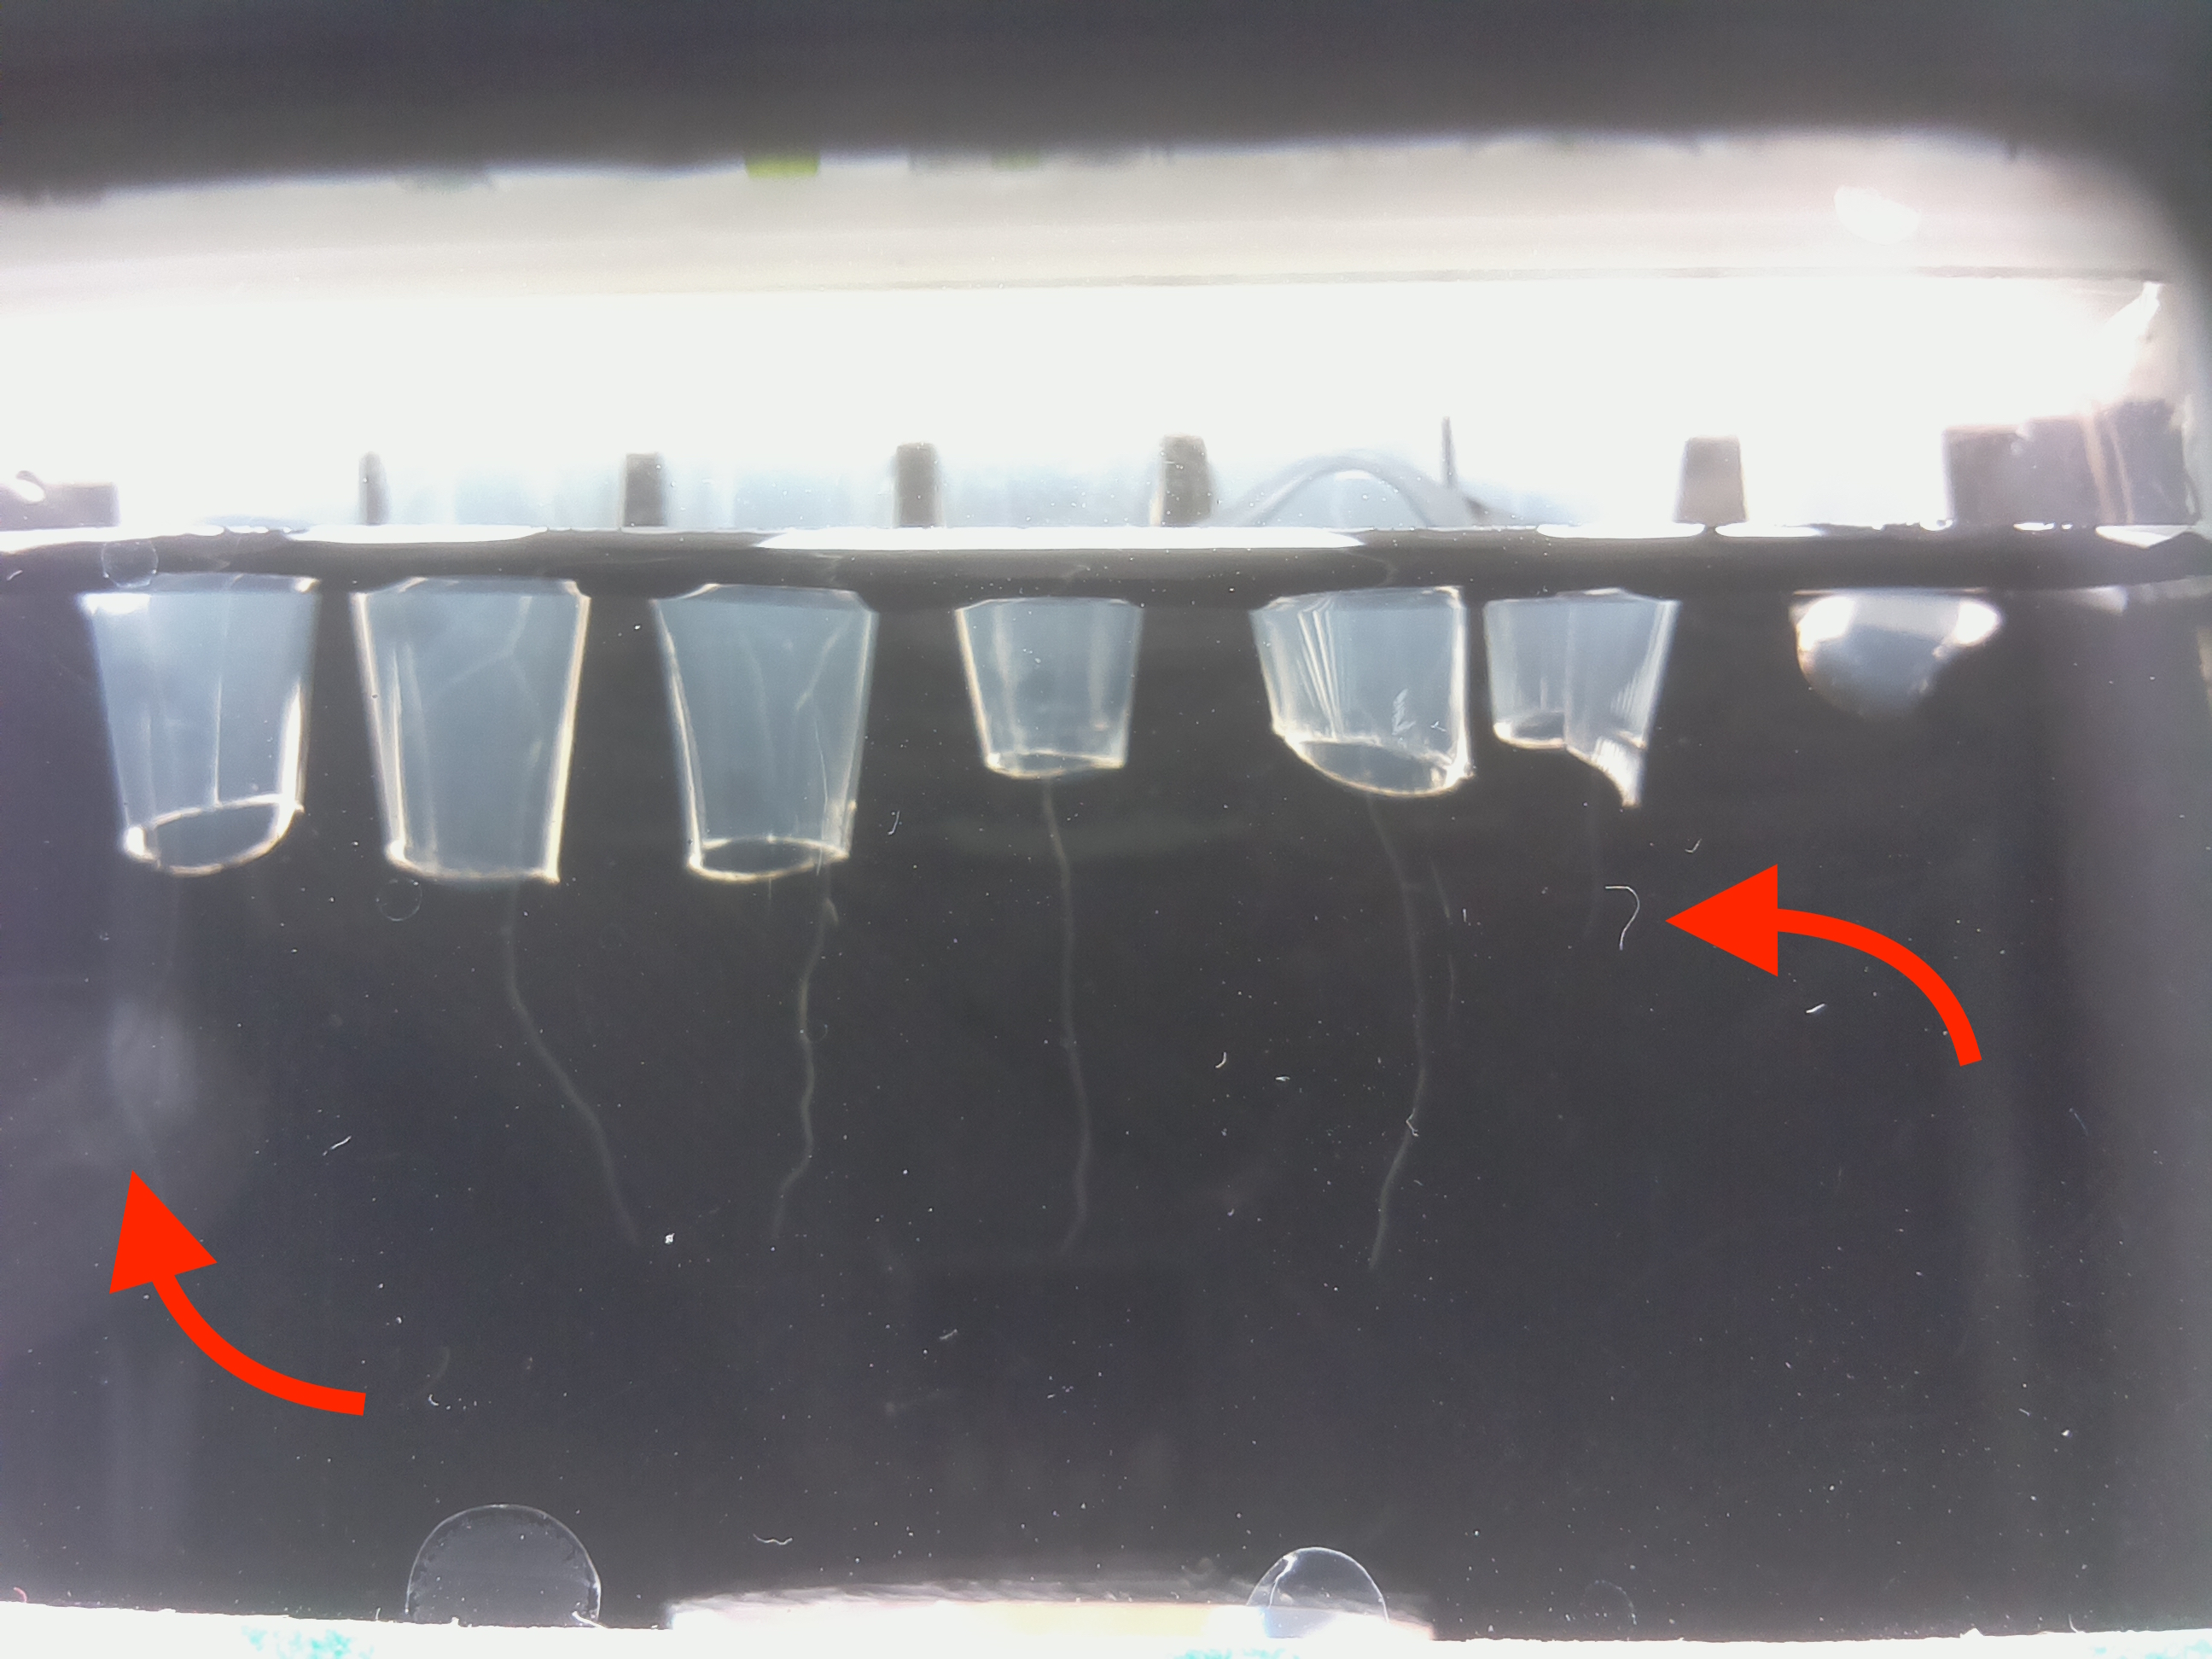
\includegraphics[width=0.75\linewidth]{2018-03-08_1000.jpg} 
		\caption{Changing light reflection (root on the LHS\\ is lost), low contrast} 
		\label{fig7:a} 
		\vspace{4ex}
	\end{subfigure}%% 
	\begin{subfigure}[b]{0.5\linewidth}
		\centering
		\includegraphics[width=0.75\linewidth]{2018-02-28_2030.jpg} 
		\caption{Foreign object sticking to root, \\blurry regions, other objects} 
		\label{fig7:b} 
		\vspace{4ex}
	\end{subfigure} 
	\begin{subfigure}[b]{0.5\linewidth}
		\centering
		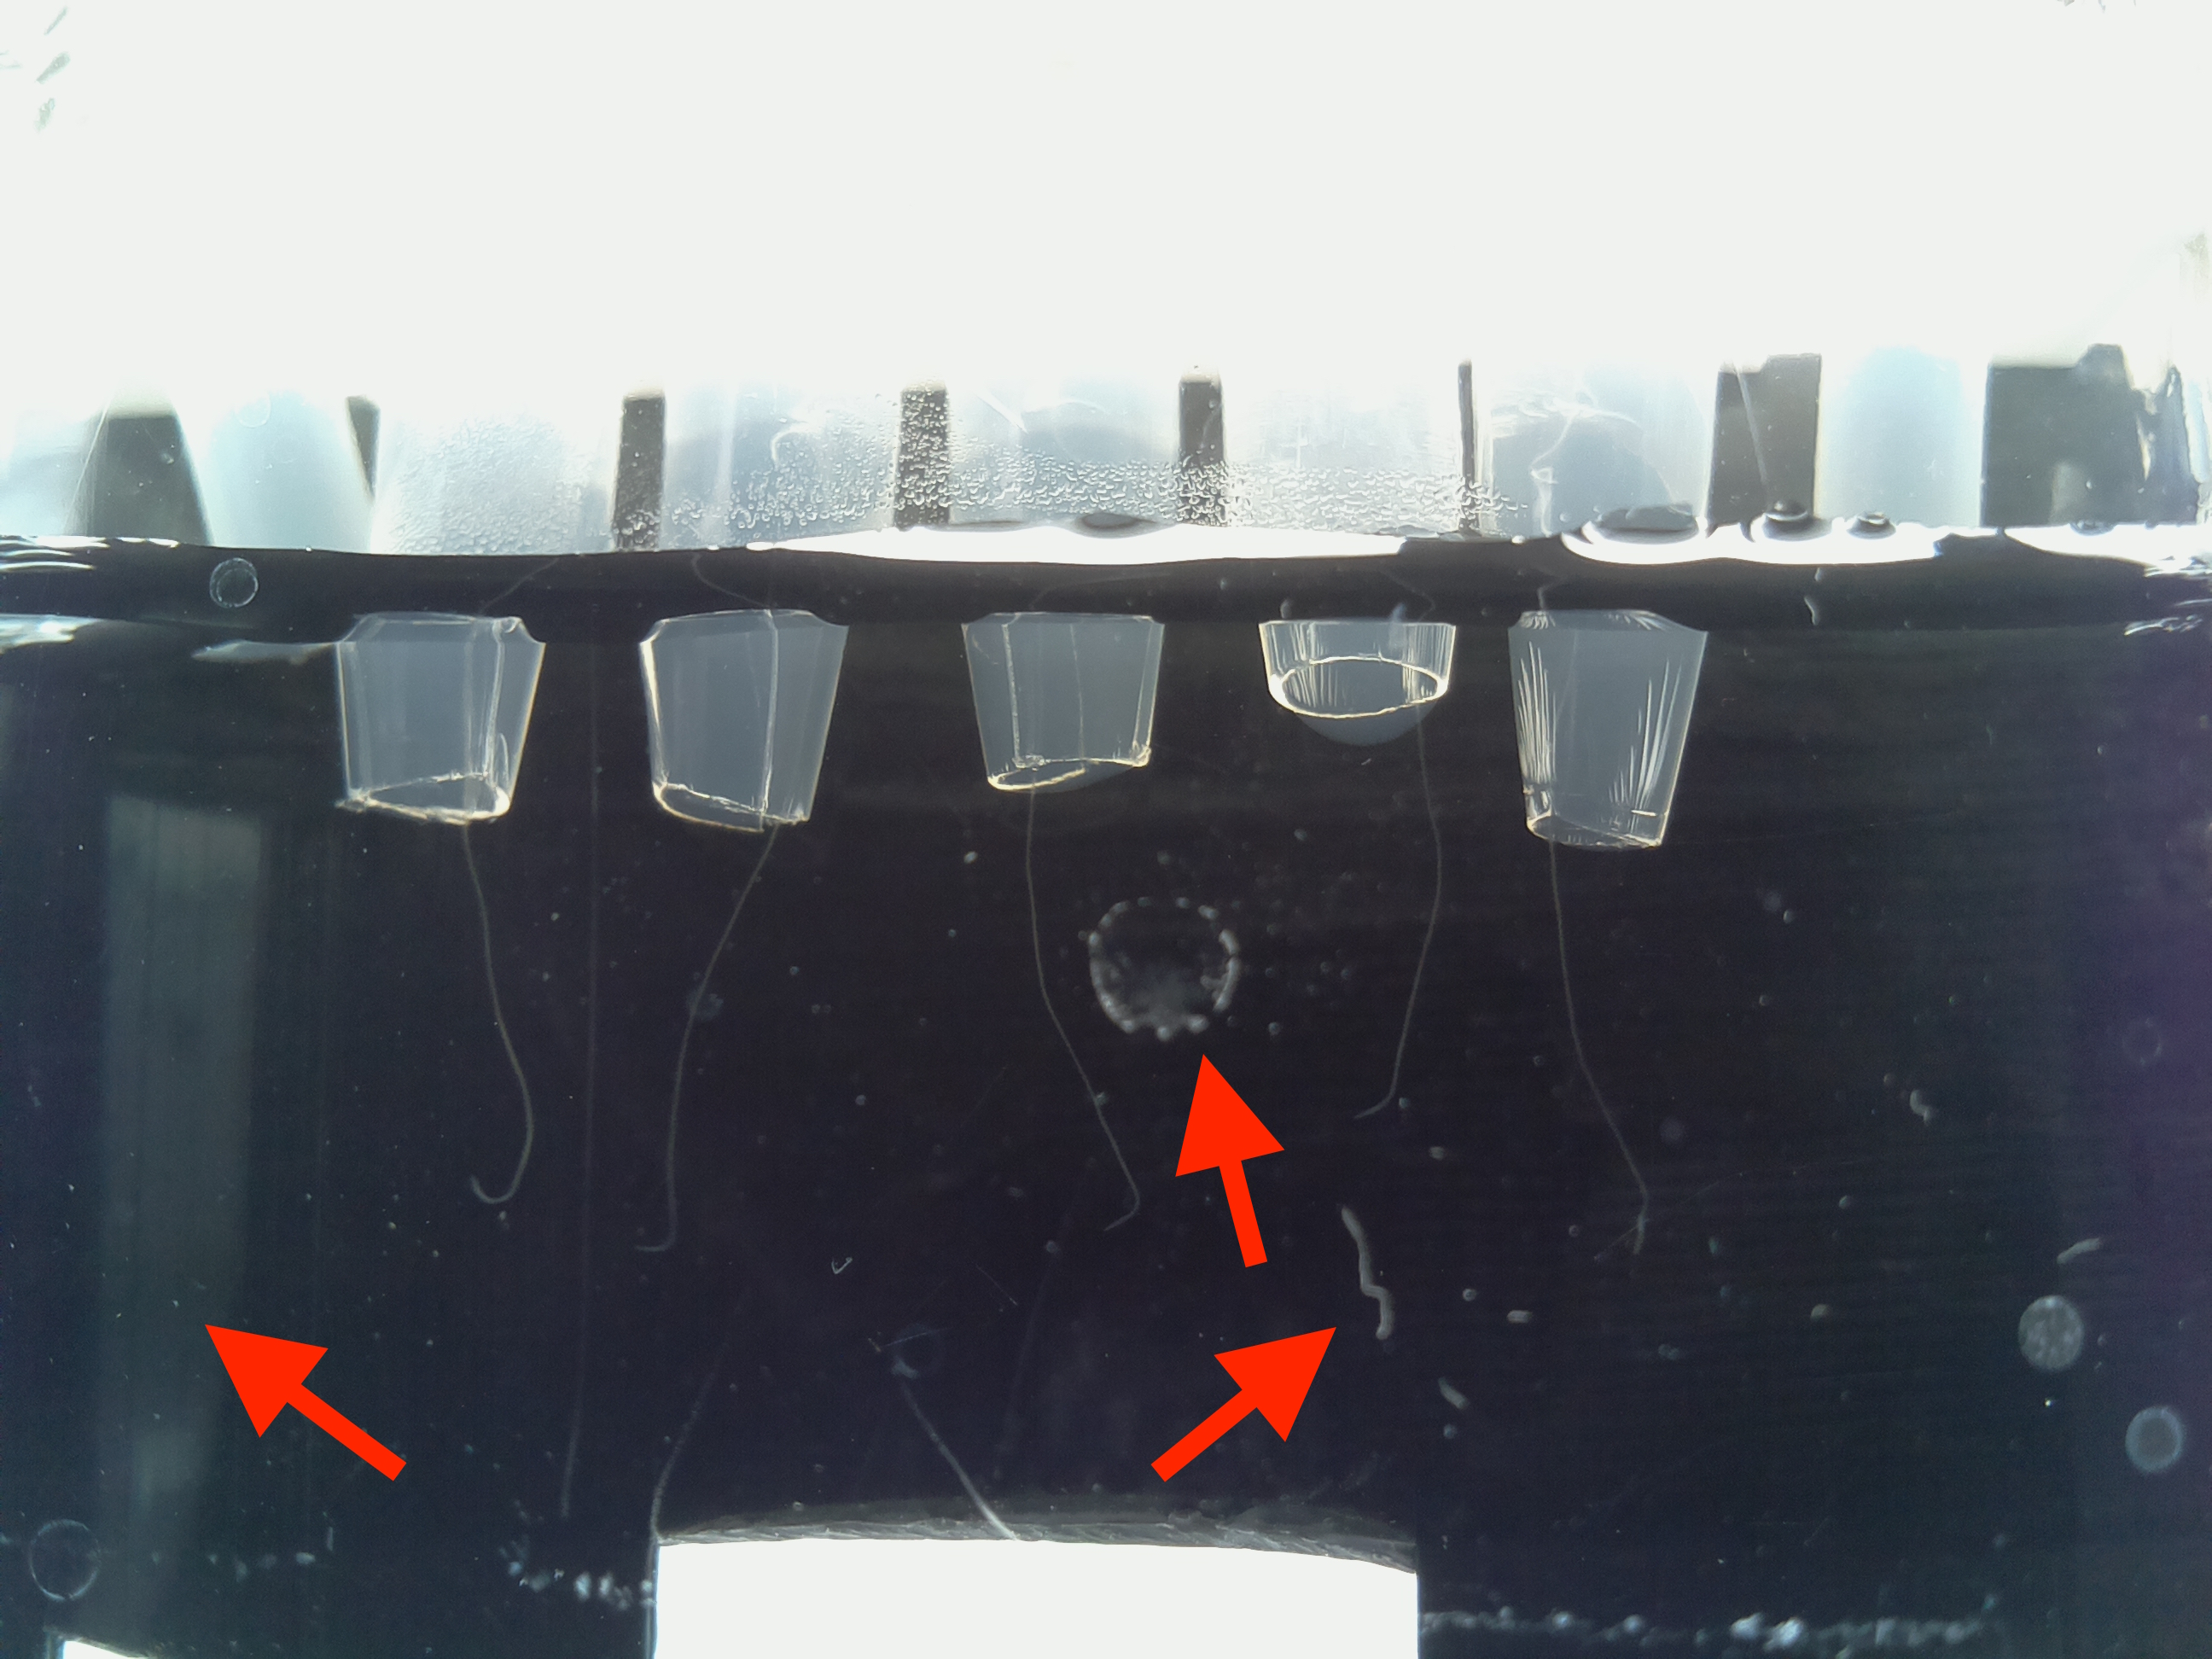
\includegraphics[width=0.75\linewidth]{2018-04-24_1840.jpg} 
		\caption{Noisy image, many objects of same colour} 
		\label{fig7:c} 
	\end{subfigure}%%
	\begin{subfigure}[b]{0.5\linewidth}
		\centering
		\includegraphics[width=0.75\linewidth]{2018-03-06_2000.jpg} 
		\caption{Low contrast, roots touching each other} 
		\label{fig7:d} 
	\end{subfigure} 
	\caption{Problems of images; images taken from our data set: (A) 2018-03-08\_1000.jpg, (B) 2018-02-28\_2030.jpg, (C) 2018-04-24\_1840.jpg, (D) 2018-03-06\_2000.jpg}
	\label{fig7} 
\end{figure}


%Eg specs not so much of an issue as separate from the root. Issue when it is connected.


%----------------------------------------------------------------------------------------
\subsection{Scalability and reproducibility}

The variation in the noise pattern in the images made it difficult to automate the process of extracting the root skeleton; every image is unique and needs to be treated uniquely. The developed pipeline works well on many images; other images require special and longer treatment. Scalability has been and continues to be a challenge.

Even though our angle computation is deterministic %and straight-forward 
and only depends on the root skeleton, there is still some variability in the preprocessing step due to the user's input. This means, it can happen that for the very same root in the very same image we get slightly different angles due to slightly different root skeletons. %This is due to the fact that our current version of \textit{RootSkel} does require user input for the preprocessing steps, meaning results of the root skeleton might slighly vary depending on the user's input.
However, the error in the angles we observed is tiny and within reasonable bounds to be negligible; we expect the measurement error to be much smaller than in the manual computations. Having said that, reproducibility can not be fully guaranteed. %; errors should be quantified for each of the methods to make a valid claim regarding robustness and actual improvement in the angle computation. 
%INSERT ERROR COMPUTATION NECESSARY, SHOW THAT OUR METHOD IS MORE ROBUST, LESS MEASUREMENT ERROR/ CLOSER TO THE TRUE THEORETICAL VALUE THATN NECESSARY


%COMMENTED OUT DUE TO WORD COUNT
%%----------------------------------------------------------------------------------------
%\subsection{High user-interaction}
%
%Even though \textit{RootSkel} comes with a lot of flexibility and simplicity in the user interaction, it would be desirable to have less user input to guarantee reproducibility and save time in the process overall. 
%
%This might overall be improved by images of higher quality in the future as well as implementing approaches that try to automate the whole preprocessing process.



%Might be reduced with better-quality images, however very flexible.


%standard-deviation not as high as i think?

%Would be desirable if it could be automated more. 


 
%----------------------------------------------------------------------------------------
%----------------------------------------------------------------------------------------
\section{Further work}

In the following we will outline suggestions for future work including things that need optimisation or features that might be nice to implement in the future. 

%COMMENTED OUT DUE TO WORD COUNT, see point below
%%----------------------------------------------------------------------------------------
%\subsection{Use more shape-based filters}
%
%To overcome the problem of separating the root from the background and the noise, one should use and optimise specific shape-based filters [AS USED IN.. INSERT REFERENCE HERE] instead of a series of colour and intensity filters that have shown to be not very efficient on our data set. This is due to the observation that the tubular structure is the most distinctive feature of the roots. Tubular structure recognising filters have been implemented but there is room for improvement. This might help to extract the skeleton more easily and reliably without the need of optional cropping or cleaning.


%%----------------------------------------------------------------------------------------
%\subsection{Effective noise reduction}
%
%In order to tackle the problem of noise reduction, it might be advisable to consult an expert not only on image processing but especially in the field of noise reduction to effectively implement filters that get rid of the noise our images contain. 
%
%%COMMENTED OUT DUE TO WORD COUNT
%%To overcome the problem of separating the root from the background and the noise, one should use and optimise specific shape-based filters [AS USED IN.. INSERT REFERENCE HERE] instead of a series of colour and intensity filters that have shown to be not very efficient on our data set. This is due to the observation that the tubular structure is the most distinctive feature of the roots. Tubular structure recognising filters have been implemented but there is room for improvement. This might help to extract the skeleton more easily and reliably without the need of optional cropping or cleaning.
%
%%EXPLOIT FACT THAT TIME SERIES IMAGE


%----------------------------------------------------------------------------------------
\subsection{Less user input up to automatisation}

Here in the first version of \textit{RootSkel}, the main goal was to standardise the angle computation. If in the future  a method for handling the different noise patterns in the images was efficiently handled which required less user input; it would be desireable to automate the whole angle computation.

In order to tackle the problem of noise reduction, it might be advisable to consult an expert not only on image processing but especially in the field of noise reduction to effectively implement filters that get rid of the noise our images contain. 

%in order to increase robustness on unseen data (which was not the goal of this work), first, one needs to collect high-quality data and second, tweak the data 
 

%----------------------------------------------------------------------------------------
\subsection{Robustness}

%The workflow developed via  many iterations on different images and 
%elaborate pre-procecessing tool for skeletonisation
%high functionality, reiterated process
%has been overengineered on one dataset, if it should be robust on other data, it needs to be trained/ tweeked on other data.


Many iterations on different images of our data set led to an elaborate tool for the pre-processing of the roots; however, we cannot prevent the tool from failing on some images. 

If one wants to make the tool available to a wider public and make it more robust so it will work on other, unseen data (which was not the goal of this work), one might want to collect higher-quality, less noisy data in the future (for suggestions on data collection see \ref{futuredataAquis}) and investigate automated approaches. % such as adaptive thresholding. 


%High-throughput software tools that can produce objective, quantitative analyses od the resulting images are now required.


%COMMENTED OUT DUE TO WORD COUNT
%%----------------------------------------------------------------------------------------
%\subsubsection{Adaptive thresholding}
%%  Another similar approach would be to ask the user to quickly draw small ROI (rectangles) to frame each root in the inverted (much easier) image. The code could then global threshold each ROI separately and go from there.
%Before opting to take user input in the form of samples of the roots in the image, we investigated adaptive (global) thresholding on each of the root and an adaptive variable setting approach on all of the roots together to extract the root. This however failed, or would have been beyond the scope of this project. % -- the reason why we implemented a user-centric approach.
%%the way it was suggested.


%COMMENTED OUT DUE TO WORD COUNT
%%----------------------------------------------------------------------------------------
%\subsection{Maintenance and bug fixing}
%
%Even though \textit{RootSkel} is a tool that is ready to be used, and we tried to cover as many cases as possible of things that could go wrong, on some exceptional images the tool might still exhibit bugs that need fixing.
%As we commented the code generously and kept log files about all changes and decisions made, a future developer should not have any problems building upon our source code.

%INSERT BUG FIXES HERE


%COMMENTED OUT DUE TO WORD COUNT
%%----------------------------------------------------------------------------------------
%\subsection{More features}
%
%More features such as a zooming in function at the beginning of force tip can be included; however, they will not change anything in the core functionality of \textit{RootSkel}.
%
%%WE HAVE INCLUDED THAT IN THE CURRENT VERSION ALREADY
%%Also, what would be nice to implement in the GUI or in an extra window from a user perspective is a graph superimposing the skeleton to illustrate which angle is computed. This way, the user can doublecheck that the correct angle is computed. This feature will be provided in the next version of \textit{RootSkel}.


%COMMENTED OUT DUE TO WORD COUNT
%%----------------------------------------------------------------------------------------
%\subsection{Other ways of curvature and angle measuring}
%
%%SHOULD WE REALLY INCLUDE THAT?
%%What was implemented as we found that this approach worked best on these data and this resolution. However, MATLAB does have some issues with singularities, e.g. whenever the angle is (exactly) 45 degrees one should doublecheck if this is due to an infinity issue in the arctan. 
%
%For the future, we might want to exploit the fact that we have time series data for the angle computation. This means that technically, it does not require the computation of the angle in each single image but only the difference in the angle to the previous image, since we assume the turning point does not change over time. 
%
%Once we have higher-resolution images or a denser data set, we will also  achieve a better approximation of the real curvature. In the meantime, it might be worthwhile to investigate more maybe better approaches to compute curvatures on sparse data sets. 
%
%Also, alternative definitions instead of an emulation of the so far manually computed angle, such as the curvature itself and possibly more robust methods of computing it might be worth further looking into. 
 

%----------------------------------------------------------------------------------------
%\subsubsection{Curvature better on dense data set}
%
%% FUTURE WORK: curvature on a sparse polygon like this might not be very
%% meaningful but that does not mean it is not possible to apply the
%% discrete approximation to the derivative to compute it. 
%% The same code on a more densly samples outline will give a good
%% approximation of the curvature of the outline
%
%%Standardised and automated version of angle computation



%%%%%%%%%%%%%%%%----from here

%----------------------------------------------------------------------------------------
\subsection{Error quantification in the angle computation}

Another additional step towards validation or an integral part of taking measurements in general %and especially precision 
%to ensure repeatability of our results 
%would be to include 
is to quantify the error in the angle computation, e.g. the maximum or average error in the final result due to the changes in the pre-processing step. %This could be computed 
One can try to do achieve this empirically by trying our tool on a large amount of data to estimate the statistical error; there are ways to also try to quantify the instrumental error. 
%THIS WORK HAS STARTED ALREADY.


%COMMENTED OUT DUE TO WORD COUNT, maybe in appendix? --- DO INCLUDE IF WE STILL HAVE WORDS LEFT
%%----------------------------------------------------------------------------------------
\subsection{Other programming languages}

Even though MATLAB has several advantages, it might be worth looking into alternative non-proprietary programming languages to make the tool accessible to a wider public or other options of making the tool portable, i.e. without requiring the user to have MATLAB installed.
Alternative languages one might want to consider are \textit{Python} and \textit{Julia}. Another recommended language is \textit{OpenCV} as it is very fast and well documented. Other non-open source software such as \textit{ImageJ}, a Java based image processing program, and \textit{Avizo} which is a general-purpose commercial software application for scientific and industrial data visualisation and analysis with a nice GUI, were not investigated further in this work. 


%%%%%%%%%%%%------------------------------------------
%
%errors should be quantified for each of the methods to make a valid claim regarding robustness and actual improvement in the angle computation. 
%
%Only if the measurement errors in our 
%
%HOW QUANTIFY THAT REALLY CLOSER TO THEORETICAL VALUE. REALLY NEED .
%
%TRY TO FIT IT TO A PHYSICAL MODEL/ UFNCTION/ MEASNURE, MAKE SOME CLAIMS BASED ON A NUMBER OF ASSUMPTIONS. 
%ANY PARTICULAR VALUE IS NOT INTERESTED, OUT OF CONTEXT DOES NOT HELP US MUCH. 
%
%
%ONLY SHOW THAT PRECISE, NOT ACCURATE.
%
%WE NEED TO FIT IT AGAINST STH TO SHOW THAT ACCURATE.
%
%PRECISION IS REPEATABILITY. ACCURACY -- HOW CLOSE TO TRUE VALUE.
%
%SAY STH ABOUT PRECISION, NOT ABOUT ACCURACY
%SINCE WE HAVE NO REAL THEORETICAL VALUE
%
%
%errors should be quantified for each of the methods to make a valid claim regarding robustness and actual improvement in the angle computation. 
%
%
%WHOM IS CLOSER?
%TRY TO FIND OUT WHO IS CLOSER, WITHOUT KNOWING THE TRUE VALUE. 
%IN A PITCHBLACK ROOM WITHOUT TOUCH. IF YOU DONT KNOW WHERE THE GOBLET. 
%WE DO NOT KNOW WHICH ONE IS CLOSER TO THE TEAPOT (RUSSELS TEAPOT, burden of the proof lies with person making the claim)
%
%RUSSELS TEAPOT
%
%
%
%YOU NEED ERRORS TO SAY STH, OTHERWISE THE VALUES ARE MEANINGLESS.
%HOW CAN QUANTIFY THESE ERRORS?
%
%WORK TOWARDS PRECISION USING STANDARD DEVIATION 
%HELPS TOWARDS MEASUREMENT ERRORS, QUANTIFIE ABILITY OF MACHINE/PERSON. BUT OTHER FACTORS WHICH WE ARE NOT GOING TO TOUCH,  USING EYES, HANDS/ MOUSE.
%
%HOW TO KNOW REAL VALUE?
%ERRORS JUST SAY STUFF ABOUT MEASUREMENTS. 
%
%
%CAN'T COMPUTE ACCURACY, WE SIMPLY DON'T KNOW TRUE THEORETICAL VALUE.
%HOW CAN A MODEL LOOK LIKE IN THIS CASE?


%NICK:
%We know that my measurements contain (sometimes quite large) degrees of error, but we also know they are going to be accurate enough that they represent roughly what the root is doing. So if the root is fully aligned with the field the measurement I take should be close to 0°, if it's only made it half of the way it should be close to 45°. 
%
%
%
%This means that we can use the measurements I have taken as a guide to make sure that your computed angles are in the right sort of range to reflect what is actually happening in the experiments. 
%
%
%In terms of computing the "improvement of the angle computation", if I understand this correctly, I am not sure how you would do this and actually I'm not sure that you need to. It is much more important for us to get a product that can improve the reproducibility of our measurements (especially between different users) as opposed to something that will measure the root angles more accurately vs manual measurements. 
%
%
%%%%%%%%%%%%------------------------------------------

%----------------------------------------------------------------------------------------
%----------------------------------------------------------------------------------------
\section{Broader application of \textit{RootSkel}}

This software tool can be reused for many purposes and is not restricted to root detection.
It might also be used for "easier" problems like analysing gravitropism.

 
% Chapter 5: CONCLUSION

\chapter{Conclusion} % Main chapter title

\label{conclusion} % For referencing the chapter elsewhere, use \ref{Chapter1} 

%%----------------------------------------------------------------------------------------
%
%% Define some commands to keep the formatting separated from the content 
%\newcommand{\keyword}[1]{\textbf{#1}}
%\newcommand{\tabhead}[1]{\textbf{#1}}
%\newcommand{\code}[1]{\texttt{#1}}
%\newcommand{\file}[1]{\texttt{\bfseries#1}}
%\newcommand{\option}[1]{\texttt{itshape#1}}

%%----------------------------------------------------------------------------------------

%WHAT, WHY, WHY ADVANTAGE, WHAT WAS CHALLENGE?


%%----------------------------------------------------------------------------------------


%Here we presented \textit{RootSkel} -- a novel and stand-alone image-analysis-based software tool developed in MATLAB optimised for noise-intensive electrotropism images that can compute the curvature and angle at the root tip in a standardised fashion with a user-friendly and very flexible pre-processing step to extract the skeleton of the root from possibly very noise image data sets.

Here we presented \textit{RootSkel} -- a novel stand-alone and intuitive image-analysis-based software tool developed in MATLAB to compute the curvature and angle at plant root tips in a standardised fashion. It was designed to work with noise-intensive electrotropism images and comes with a user-friendly and flexible pre-processing step to extract the skeleton of the root. % from possibly very noise image data sets.

The software has been designed using an extensive amount of different filtering techniques optimised on the image data set described in this work and can therefore be used to work with standard images from consumer digital cameras. 

Automated image capturing as well as the design of the software presented here both aim to reduce the time-consuming process of the biologist quantifying the root tip curvature manually but more importantly, it standardises the computations and makes the results reproducible and comparable over a large amount of data. It offers the possibility to extend the analysis by including different angle definitions to capture the curvature of the plant root and compare them. Also, the software tool is not limited to computing the angle of root tips but due to the flexibility of the pre-processing step can be used for any other curved or polynomial-like structure. 

Based on angles of 3 Arabidopsis roots we showed that the computed by \textit{RootSkel} do not differ significantly (p-value \(>0.05\)) from the manually compted ones and, therefore, represent a good emulation thereof.
However, the robustness and reproducibility of \textit{RootSkel} need to be further validated; suggestions for future work can be implemented. 

We hope \textit{RootSkel} will contribute to the understanding of highly complex and poorly-understood phenomenons like eletrotropism in plants and possibly other tropisms. %, as well as plant growth in general.

%.FROM ABSTRACT
%Unlike when doing the angle computation to measure the curvature of a root tip manually, our tool ensures a standardised version of the angle computation. On top of it, we  developed a user-friendly graphical user interface (GUI) that will help the user in processing the images and compute the angles in a standardised and controlled fashion.
%
%We use a data set of high-throughput time-lapse images of Arabidopsis roots from 5 experiments with 4-5 roots each containing between 32 and 36 images over a period of approximately 5 hours produced by the Plant Morphology lab at Imperial College London, we evaluate our results by comparing it to previously manually computed angles. [INCLUDE RESULTS A LA 70\% of the images could be found to be reproduced]


%HHope to be able to standardise it in the future.

 

%----------------------------------------------------------------------------------------
%	BIBLIOGRAPHY
%----------------------------------------------------------------------------------------

\printbibliography[heading=bibintoc]

%----------------------------------------------------------------------------------------

%----------------------------------------------------------------------------------------
%	THESIS CONTENT - APPENDICES
%----------------------------------------------------------------------------------------

\appendix % Cue to tell LaTeX that the following "chapters" are Appendices

% Include the appendices of the thesis as separate files from the Appendices folder
% Uncomment the lines as you write the Appendices

% Appendix A


%----------------------------------------------------------------------------------------
%----------------------------------------------------------------------------------------
%----------------------------------------------------------------------------------------
\chapter{Detailed high-level description of the components of \textit{RootSkel}}

\newpage
\begin{table}[H]
	\centering
	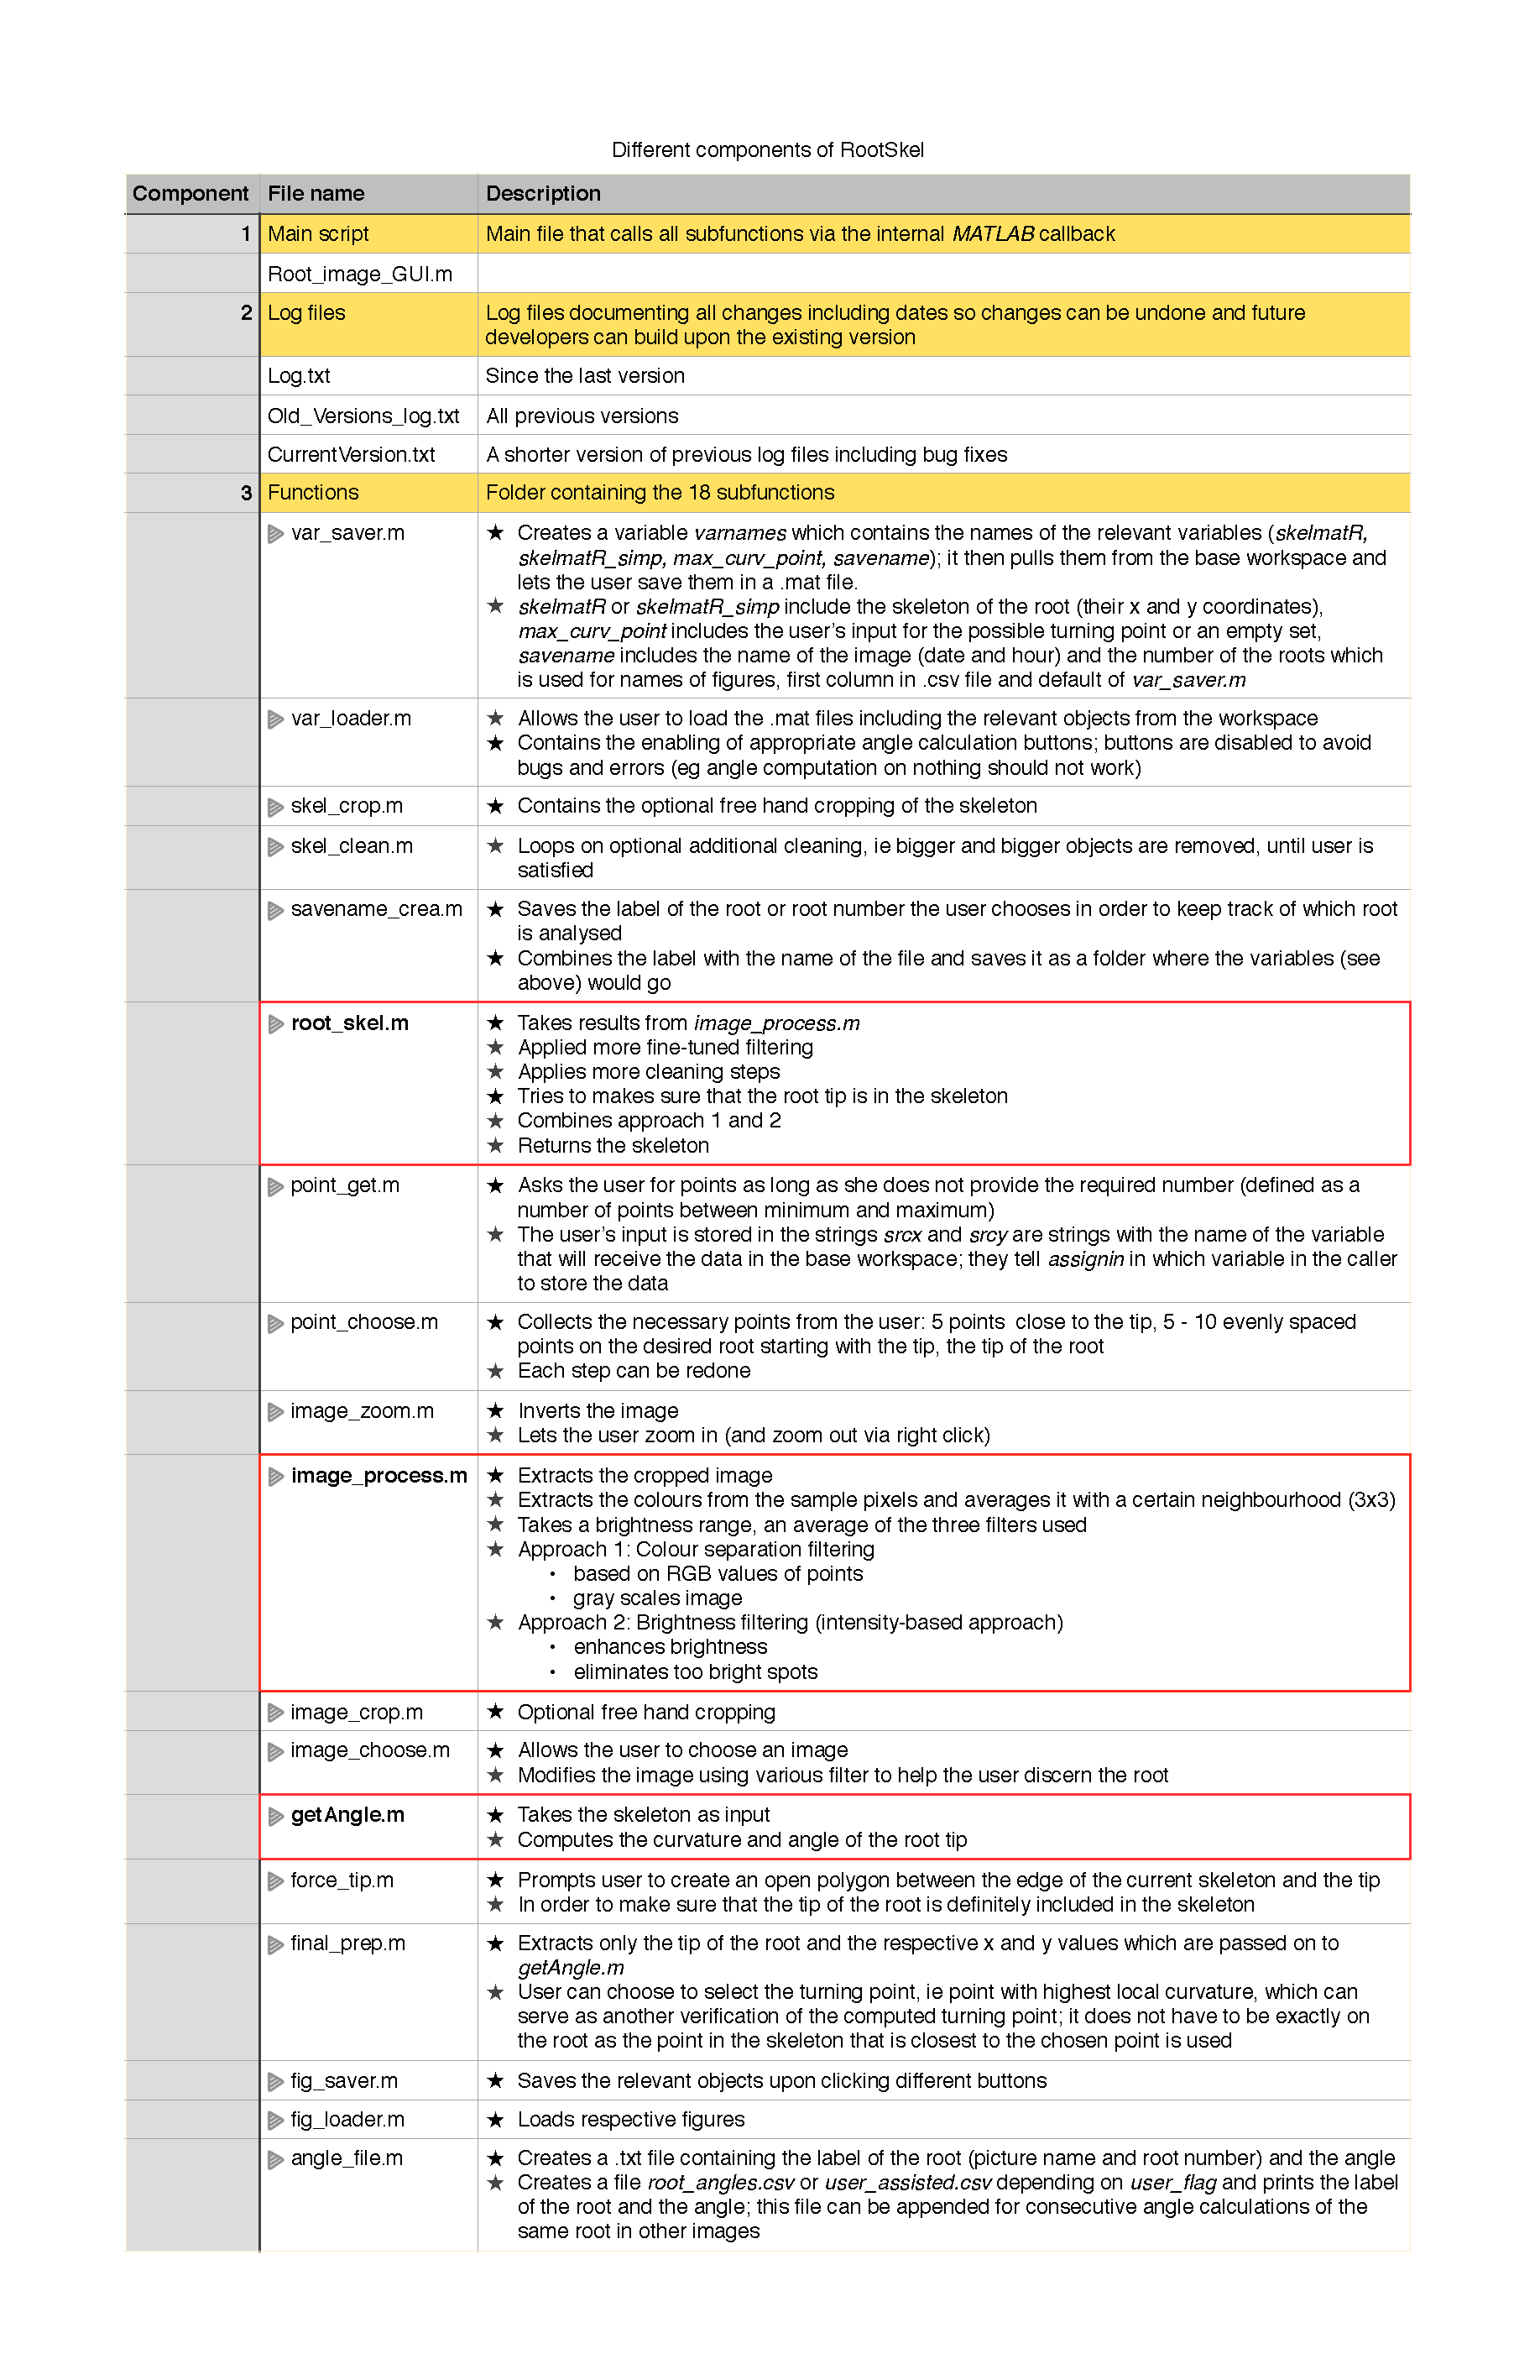
\includegraphics[width=1.\textwidth]{../Figures/components2.pdf}
	\caption{The different components and modules of \textit{RootSkel} with a description of each of them; the most important ones containing the core functionality of \textit{RootSkel} are framed in red, the high-level components are shaded in yellow. A version of an increased font size can be found on \url{https://github.com/burfel/root-tip-angle/blob/master/report/Figures/components.pdf}.}
	\label{table:modules}
\end{table}



%----------------------------------------------------------------------------------------
%----------------------------------------------------------------------------------------
%----------------------------------------------------------------------------------------
\chapter{Manual for \textit{RootSkel}}\label{chp:manual}


%----------------------------------------------------------------------------------------
%----------------------------------------------------------------------------------------
\section{Key features} %SHOW HOW ELEABORATE TOOL IS

Figure \ref{fig:workflow} explains the key components of %this image-analysis software tool 
\textit{RootSkel} to address the problem of highly noisy electrotropism consumer camera images of Arabidopsis roots and a standardised way of computing the angle for the curved root tip. 

This tool takes the form of a MATLAB program and subprograms with a graphical user interface on top of it.

%----------------------------------------------------------------------------------------
\subsection{Handling user's mistakes}

When we take the user's input, e.g. choosing samples along the root, we correct for small mistakes by taking a neighbourhood (3\(\times\)3) average around the pixel. 
%followed by adaptive thresholding.
This means the user does not have to take special care when choosing the points as long as it is in the approximate region of the root.

%----------------------------------------------------------------------------------------
\subsection{User interaction and optional steps}
The software tool was created in ways that it is easy to interact with for a future user. 
We implemented several optional steps that only need to be performed if the user thinks they are necessary. This on the one hand saves time in the preprocessing but on the other hand also ensures that tricky roots can be tackled by various optional steps in order to extract a skeleton. 

%----------------------------------------------------------------------------------------
\subsection{Drawing the angle}
The GUI lets the user visualise the angle that is computed. This not only helps to make the tool more visual and transparent, but can also assist in debugging. 



%%----------------------------------------------------------------------------------------
%%----------------------------------------------------------------------------------------
%%----------------------------------------------------------------------------------------
%\chapter{Other programming languages}
%
%Even though MATLAB has several advantages, it might be worth looking into alternative non-proprietary programming languages to make the tool accessible to a wider public or other options of making the tool portable, i.e. without requiring the user to have MATLAB installed.
%Alternative languages one might want to consider are \textit{Python} and \textit{Julia}. Another recommended language is \textit{OpenCV} as it is very fast and well documented. Other non-open source software such as \textit{ImageJ}, a Java based image processing program, and \textit{Avizo} which is a general-purpose commercial software application for scientific and industrial data visualisation and analysis with a nice GUI, were not investigated further in this work. 


%----------------------------------------------------------------------------------------
%----------------------------------------------------------------------------------------
\section{\textit{RootGUI} for Dummies}

%REMARK: For environmental reasons, we do not show \textit{RootGUI}, the manual of \textit{RootSkel} in the printed version. We refer to the electronic version to view the easy to read and fun \textit{RootGUI} for Dummies manual.

%----------------------------------------------------------------------------------------
\subsection{Intro}

Hello and welcome! 
So this is is your first time operating \textit{RootGUI}, the GUI of \textit{RootSkel}. Excited?
For the next 5 minutes or so I'll be your friendly instruction manual on how to use \textit{RootGUI}. 
You have donloaded the current version of \textit{RootSkel} from \url{https://github.com/GiovanniSena/Auto-angle} and you have MATLAB installed on your computer? Then let's get right down to business.

First of all, open your \textit{MATLAB}. You should view something similar to this::
\begin{figure}[H]
	\centering
	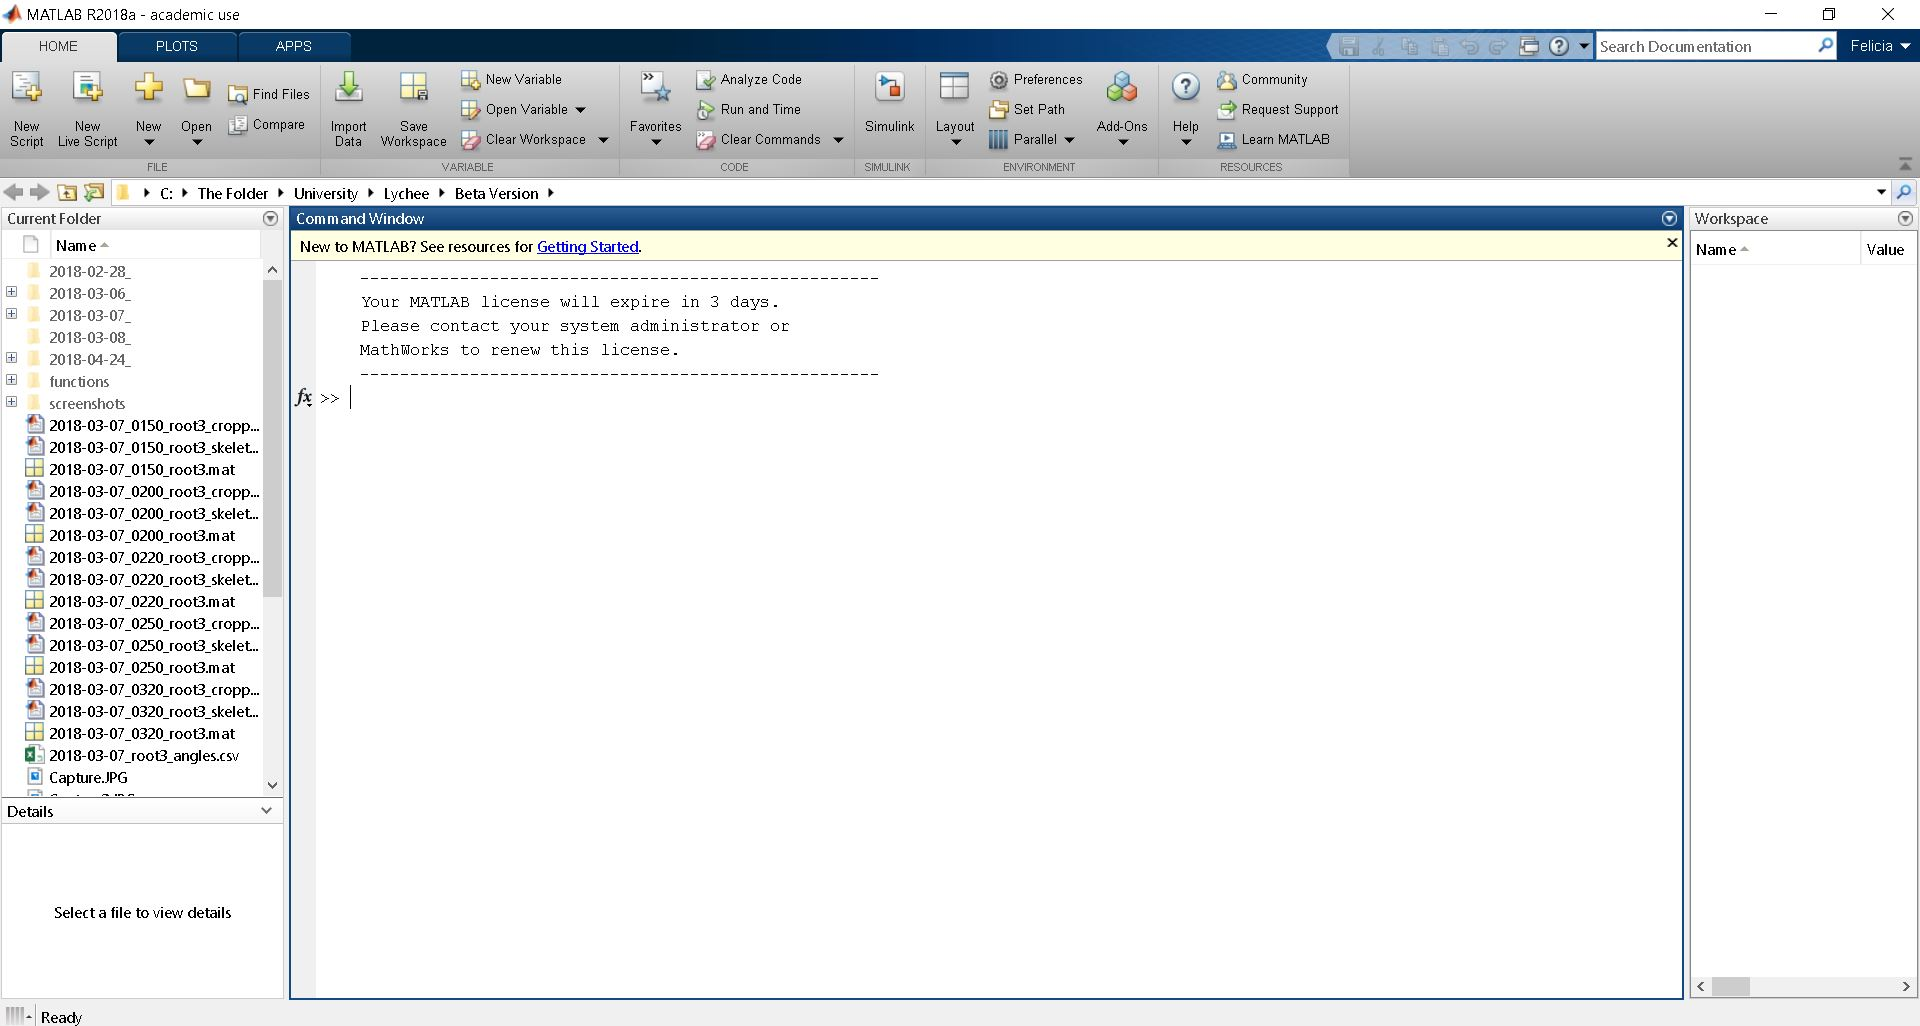
\includegraphics[width=\textwidth]{../Figures/manual/intro1.jpg}
	\caption{The MATLAB GUI}
	\label{fig:img1}
\end{figure}

And now, in order to bring \textit{RootGUI} up, navigate to the folder where \textit{RootSkel} is lovated on the LHS, and type \textit{Root\_image\_GUI} in the MATLAB console as shown in figure \ref{fig:img2}.
\begin{figure}[H]
	\centering
	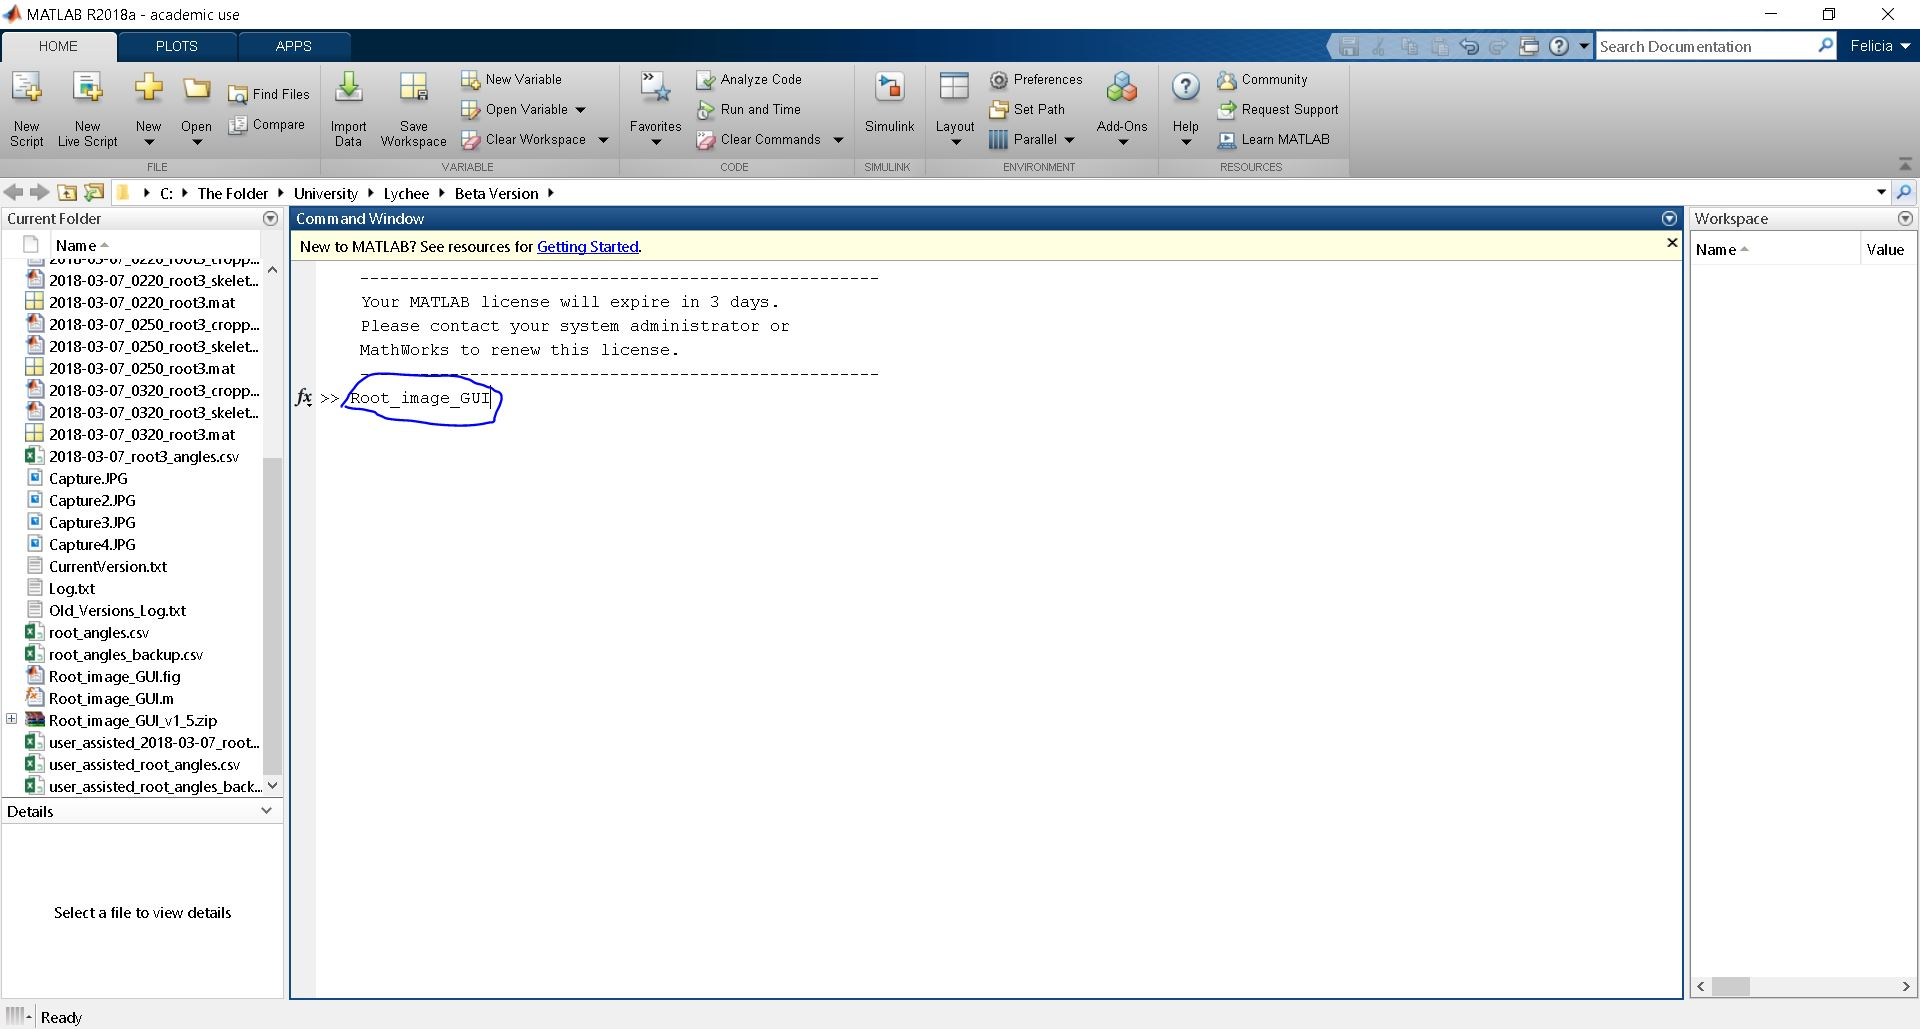
\includegraphics[width=\textwidth]{../Figures/manual/intro2.jpg}
	\caption{Calling \textit{Root\_image\_GUI} from the MATLAB console}
	\label{fig:img2}
\end{figure}

Then press enter and voil\`a!
\begin{figure}[H]
	\centering
	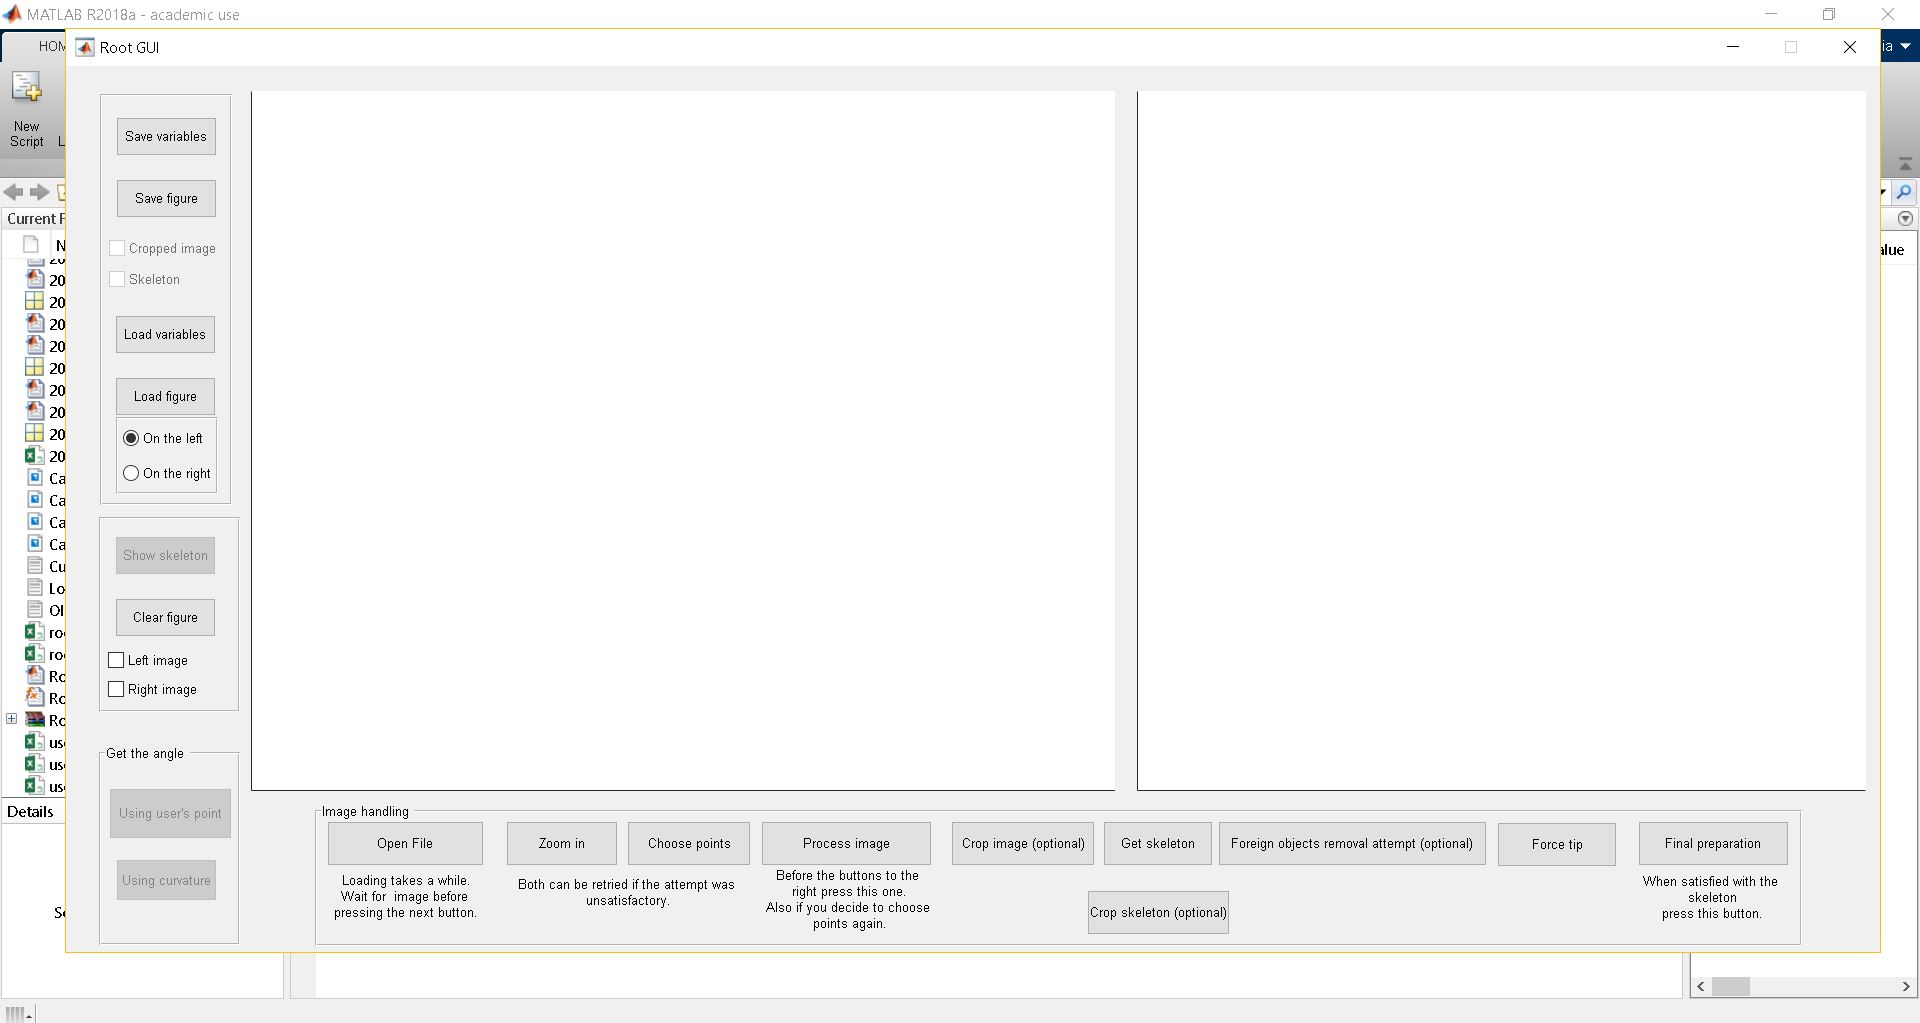
\includegraphics[width=\textwidth]{../Figures/manual/intro3.jpg}
	\caption{The \textit{RootGUI}}
	\label{fig:img3}
\end{figure}

There you go, you have opened the GUI! You've successfully completed the first step.

%----------------------------------------------------------------------------------------
Now let's get ourselves some angles.
\subsection{Getting the angles -- main route}

First, we want to open an image with the roots.
 \begin{figure}[H]
 	\centering
 	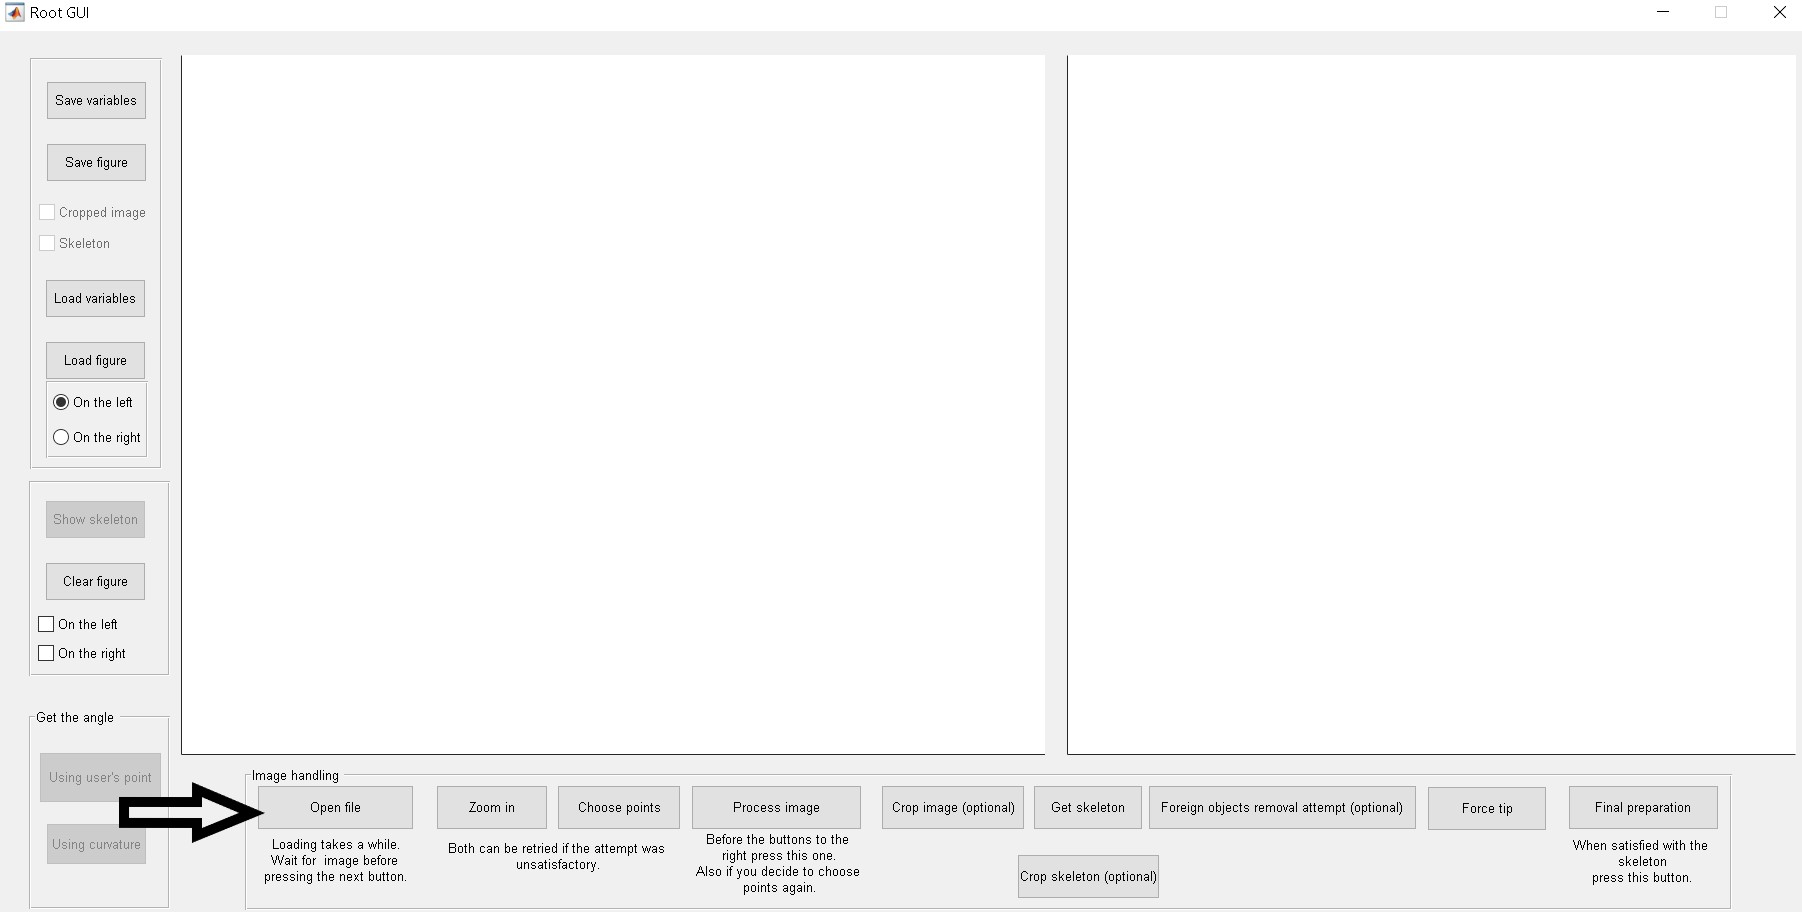
\includegraphics[width=\textwidth]{../Figures/manual/step1.jpg}
 	\caption{Step 1 in the \textit{RootSkel} pipeline: Opening a file}
 	\label{fig:img4}
 \end{figure}
 
 We click the \textit{Open file} button and you are prompted to choose an image.
 \begin{figure}[H]
 	\centering
 	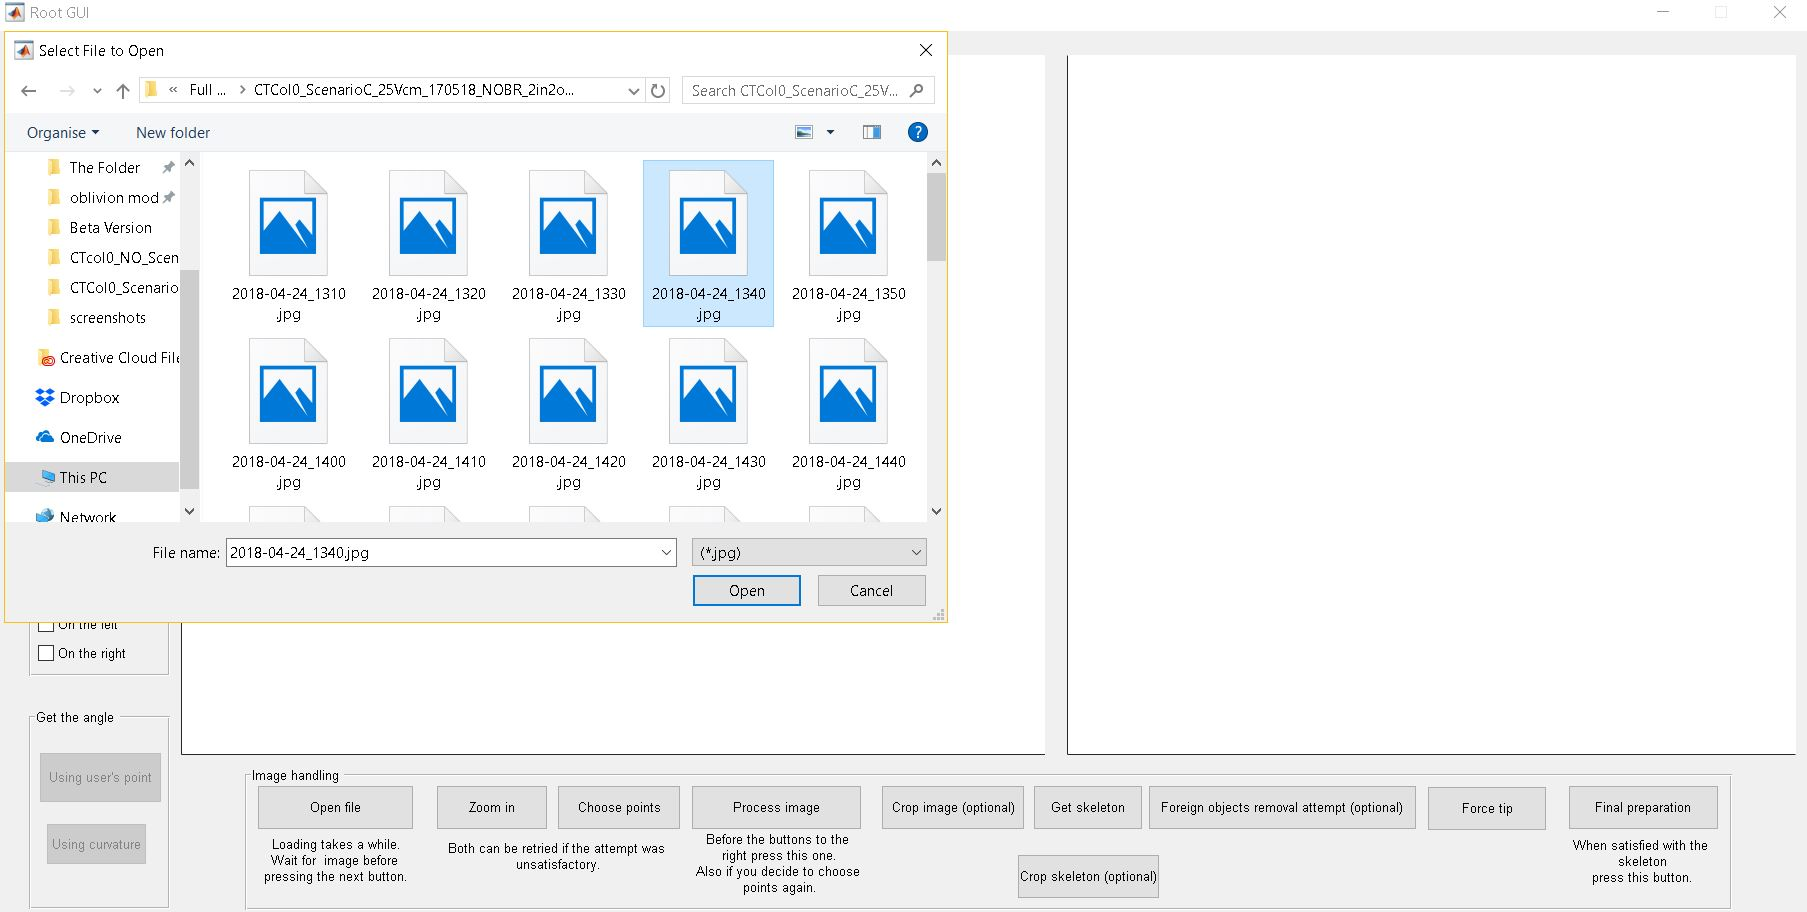
\includegraphics[width=\textwidth]{../Figures/manual/step2.jpg}
 	\caption{Choosing a file}
 	\label{fig:img5}
 \end{figure}
 
 Now that we chose our image, the next thing we should do is to zoom in on the root we want to work on. 
 For that, we click on the \textit{Zoom in} button.
 \begin{figure}[H]
 	\centering
 	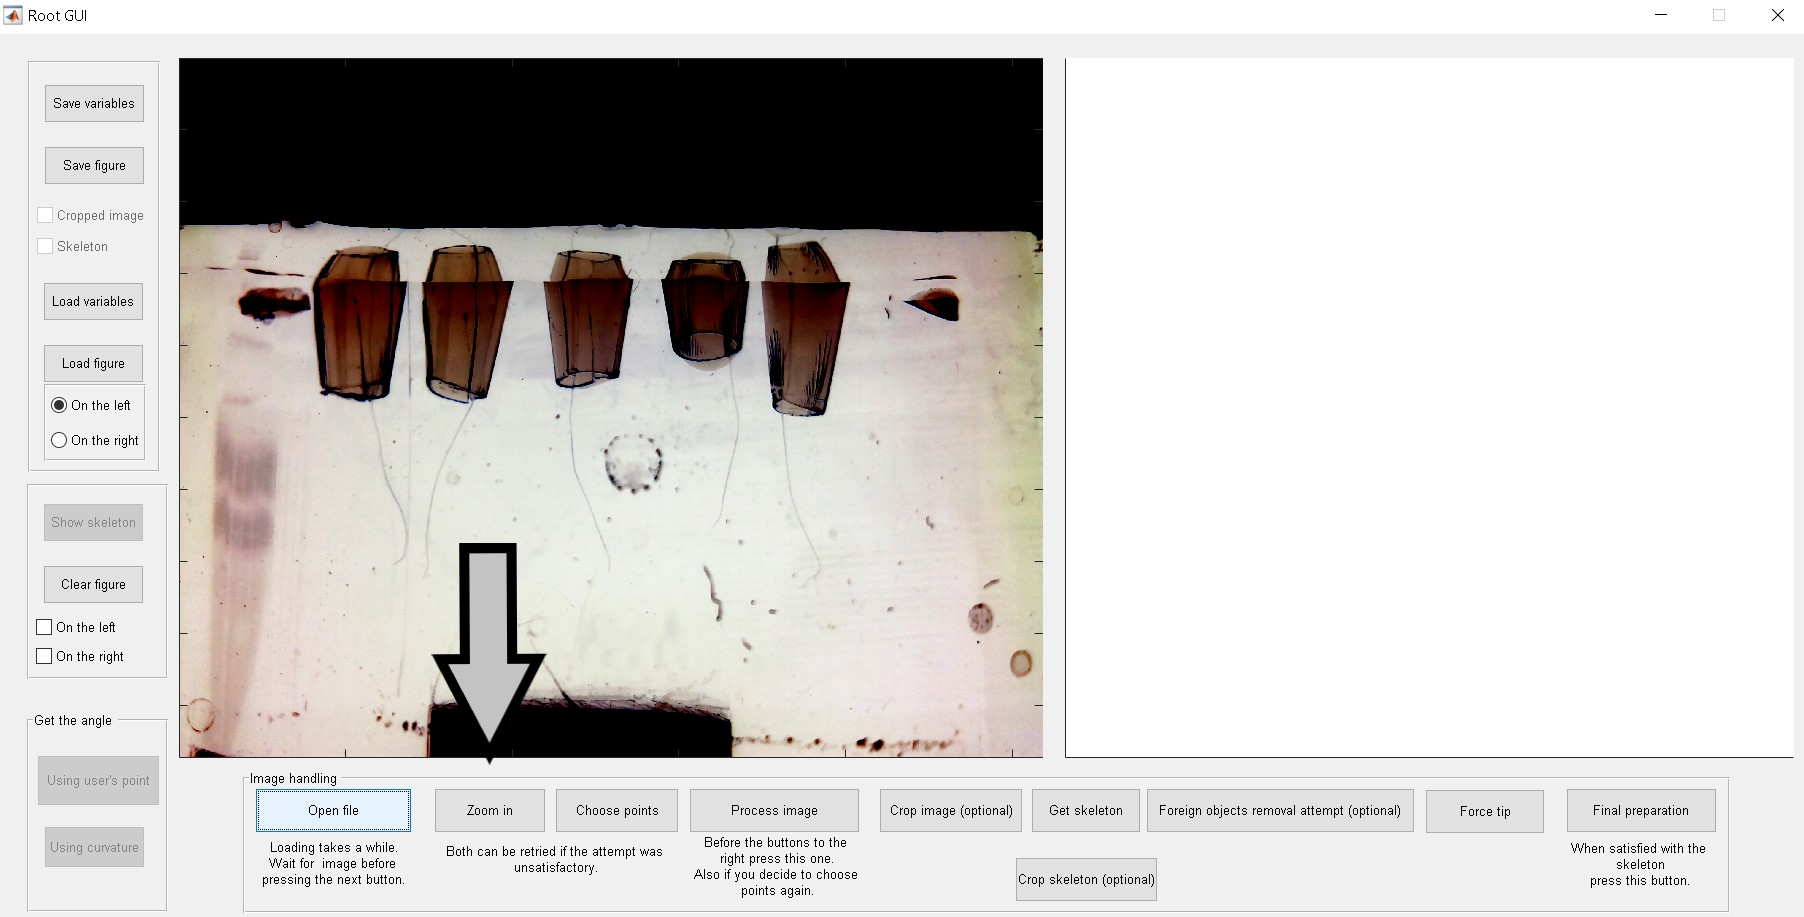
\includegraphics[width=\textwidth]{../Figures/manual/step3.jpg}
 	\caption{Step 2 in the \textit{RootSkel} pipeline: Zooming in on the desired root}
 	\label{fig:img6}
 \end{figure}
 
 After you clicked the button, you will be prompted to zoom in on the desired root (see figure \ref{fig:img7}
 and you will go on to drag a rectangle around the desired root (see figure \ref{fig:img8} -- \ref{fig:img15}).
 	
\begin{figure}[H]
 	\centering
 	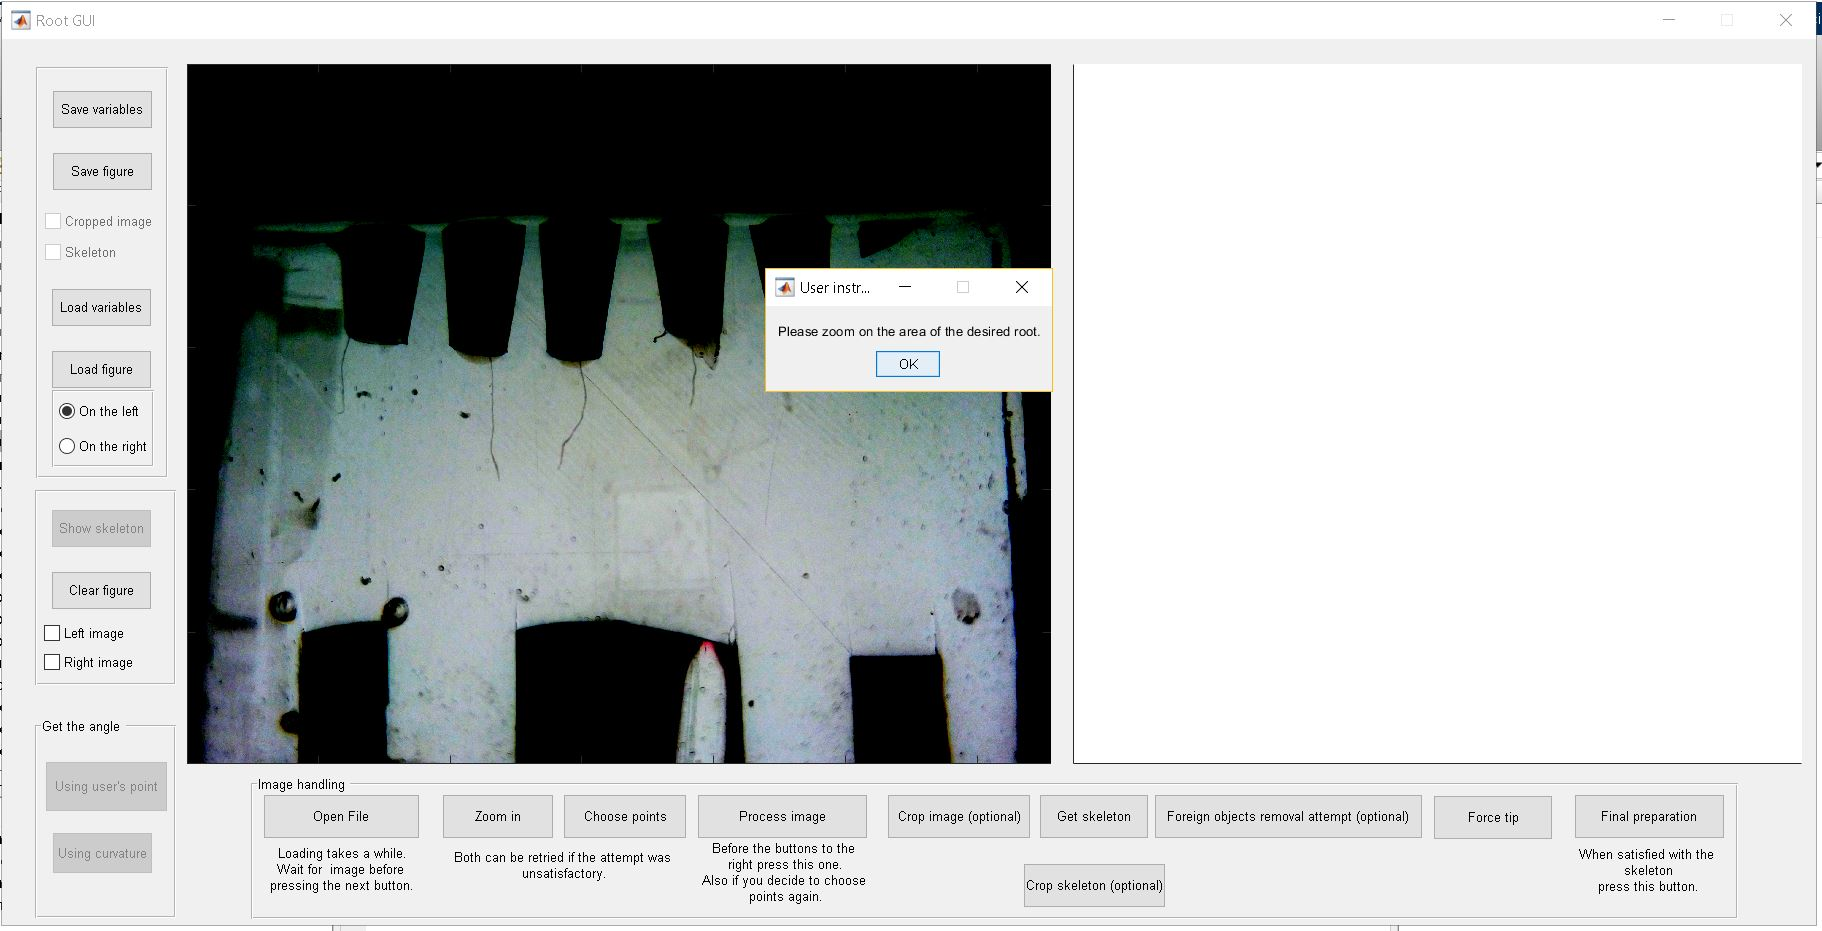
\includegraphics[width=\textwidth]{../Figures/manual/step4.jpg}
 	\caption{Prompt to zoom in on the dedired root}
 	\label{fig:img7}
\end{figure} 	
 
\begin{figure}[H]
  	\centering
  	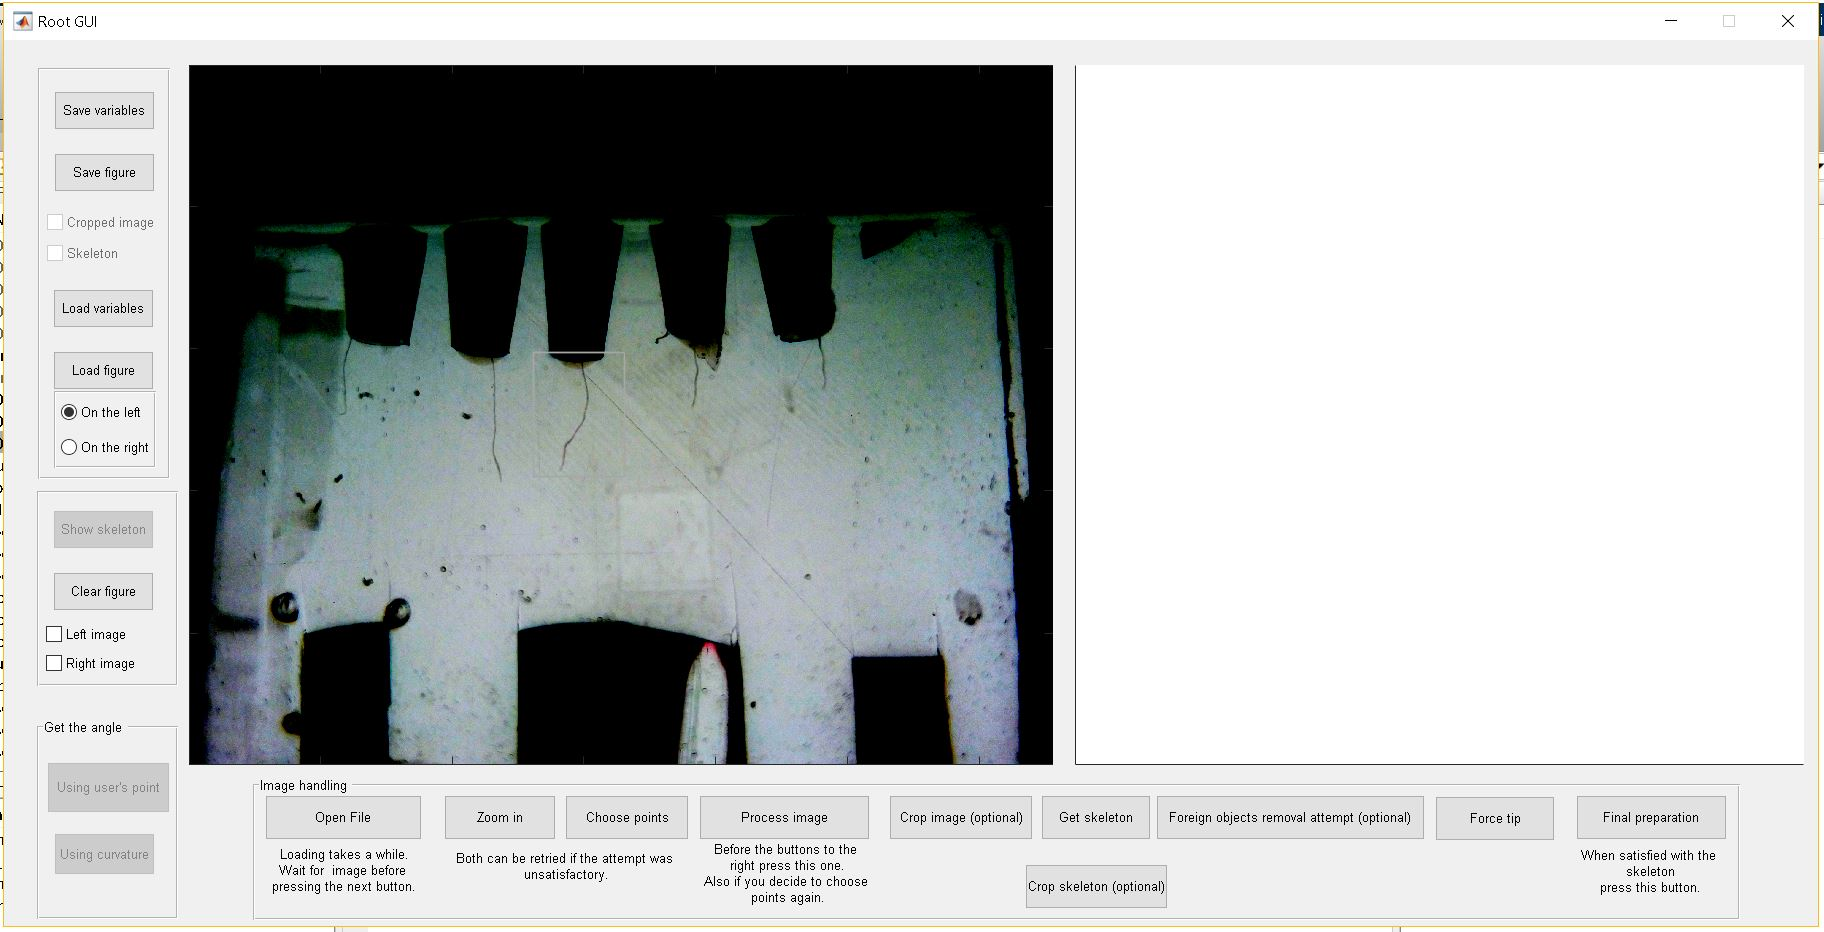
\includegraphics[width=\textwidth]{../Figures/manual/step5.jpg}
  	\caption{Drawing a rectangle around the desired root}
  	\label{fig:img8}
\end{figure}
  
Now that that's done, we want to choose points to give our program some data so that it will be able to pre-process the image.
Click the \textit{Choose points} button and follow the instructions that will appear on the screen: Choose as many roots as the instruction tells you, and on the last step only the tip of the root (see figures \ref{fig:img9})

\begin{figure}[H]
	\centering
	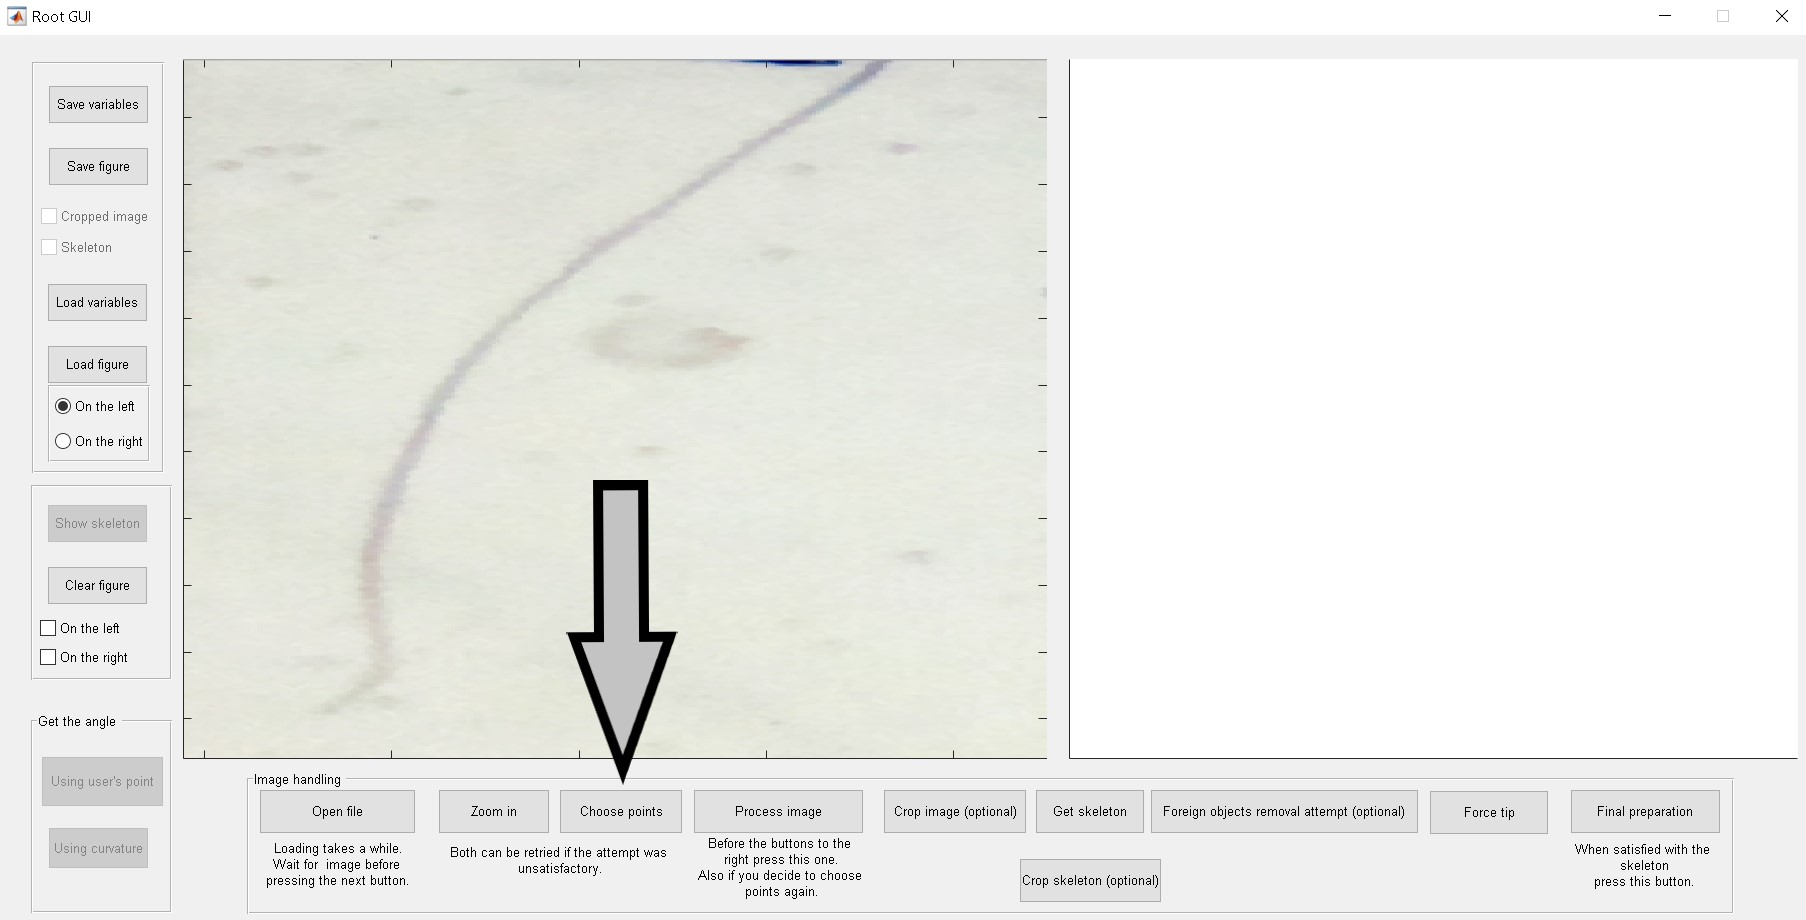
\includegraphics[width=\textwidth]{../Figures/manual/step6.jpg}
	\caption{Step 3 in the \textit{RootSkel} pipeline: Choosing points along the root}
	\label{fig:img9}
\end{figure}

\begin{figure}[H]
	\centering
	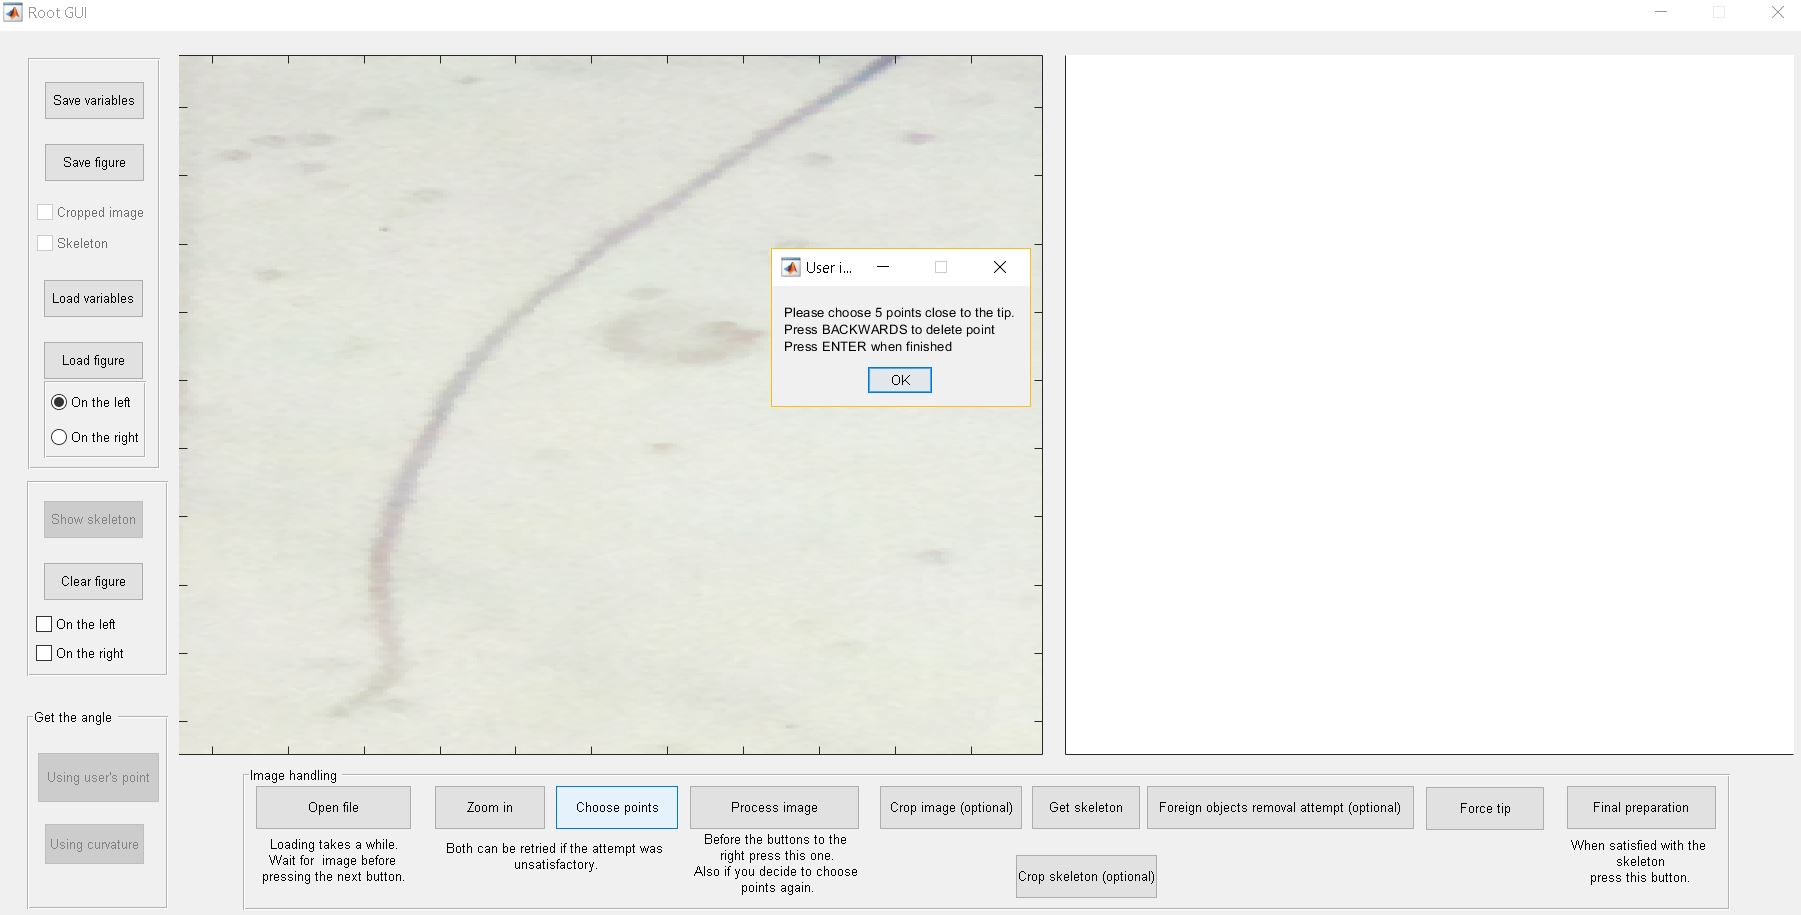
\includegraphics[width=\textwidth]{../Figures/manual/step7.jpg}
	\caption{Prompt to choose 5 points close to the tip of the root}
	\label{fig:img10}
\end{figure}

\begin{figure}[H]
	\centering
	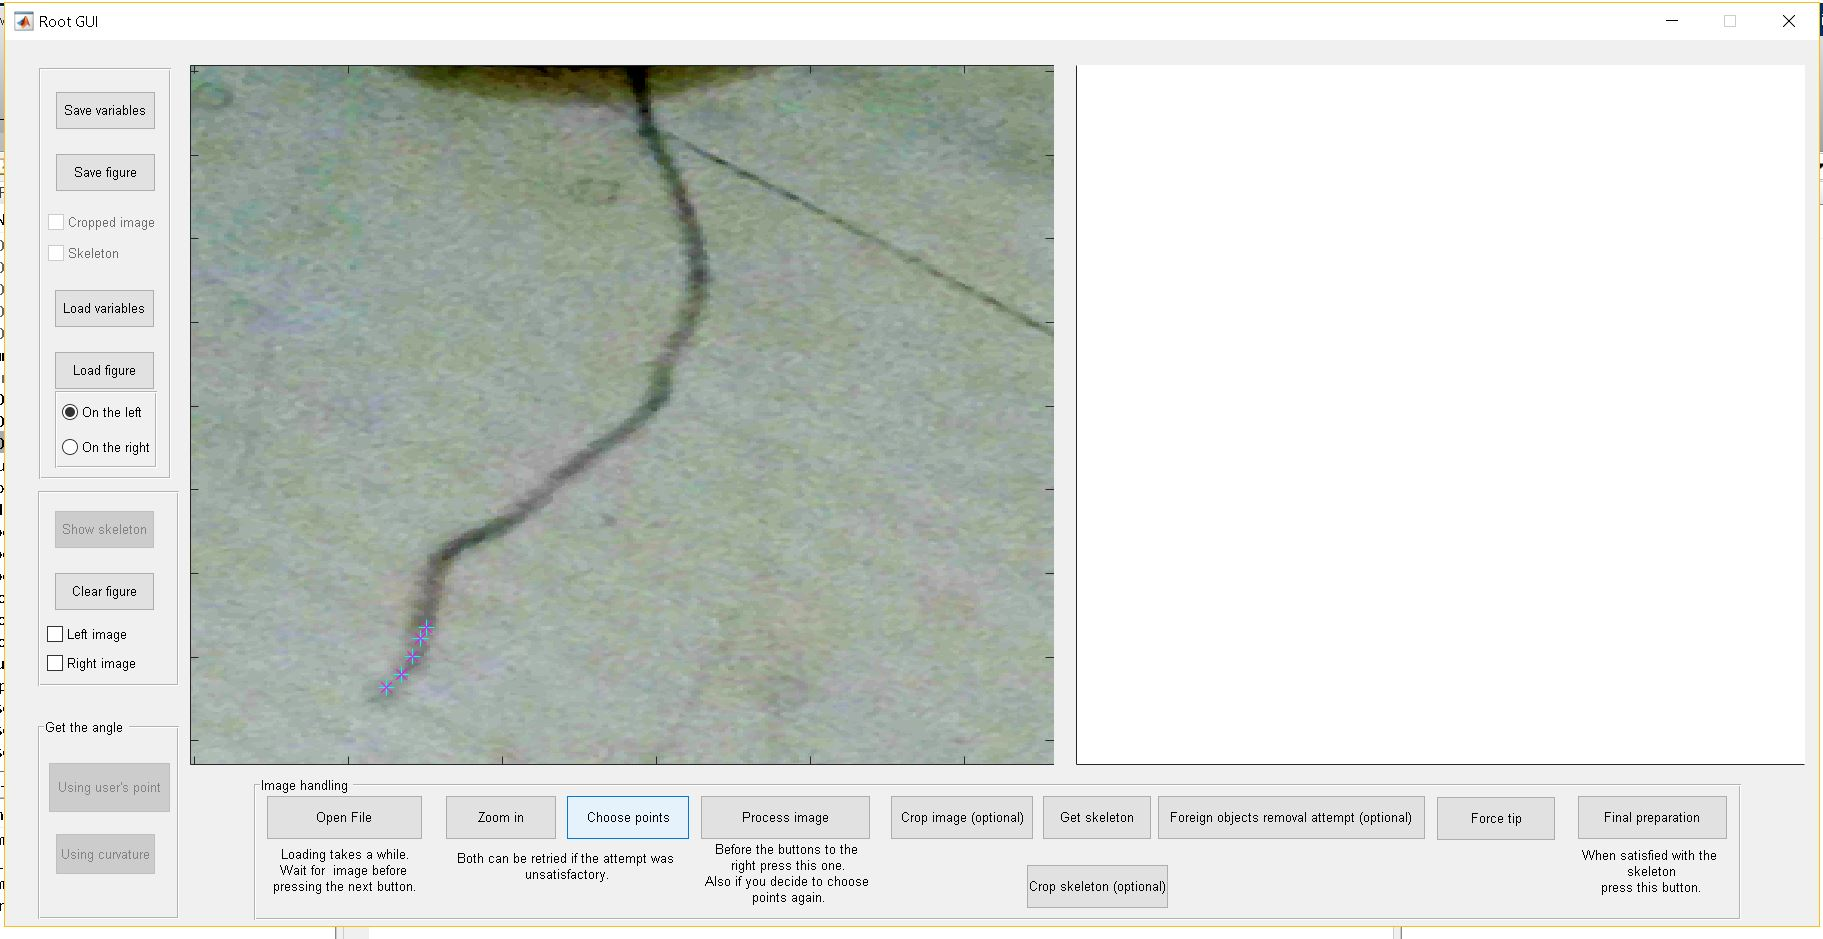
\includegraphics[width=\textwidth]{../Figures/manual/step8.jpg}
	\caption{After choosing the 5 points close to the tip}
	\label{fig:img11}
\end{figure}

\begin{figure}[H]
	\centering
	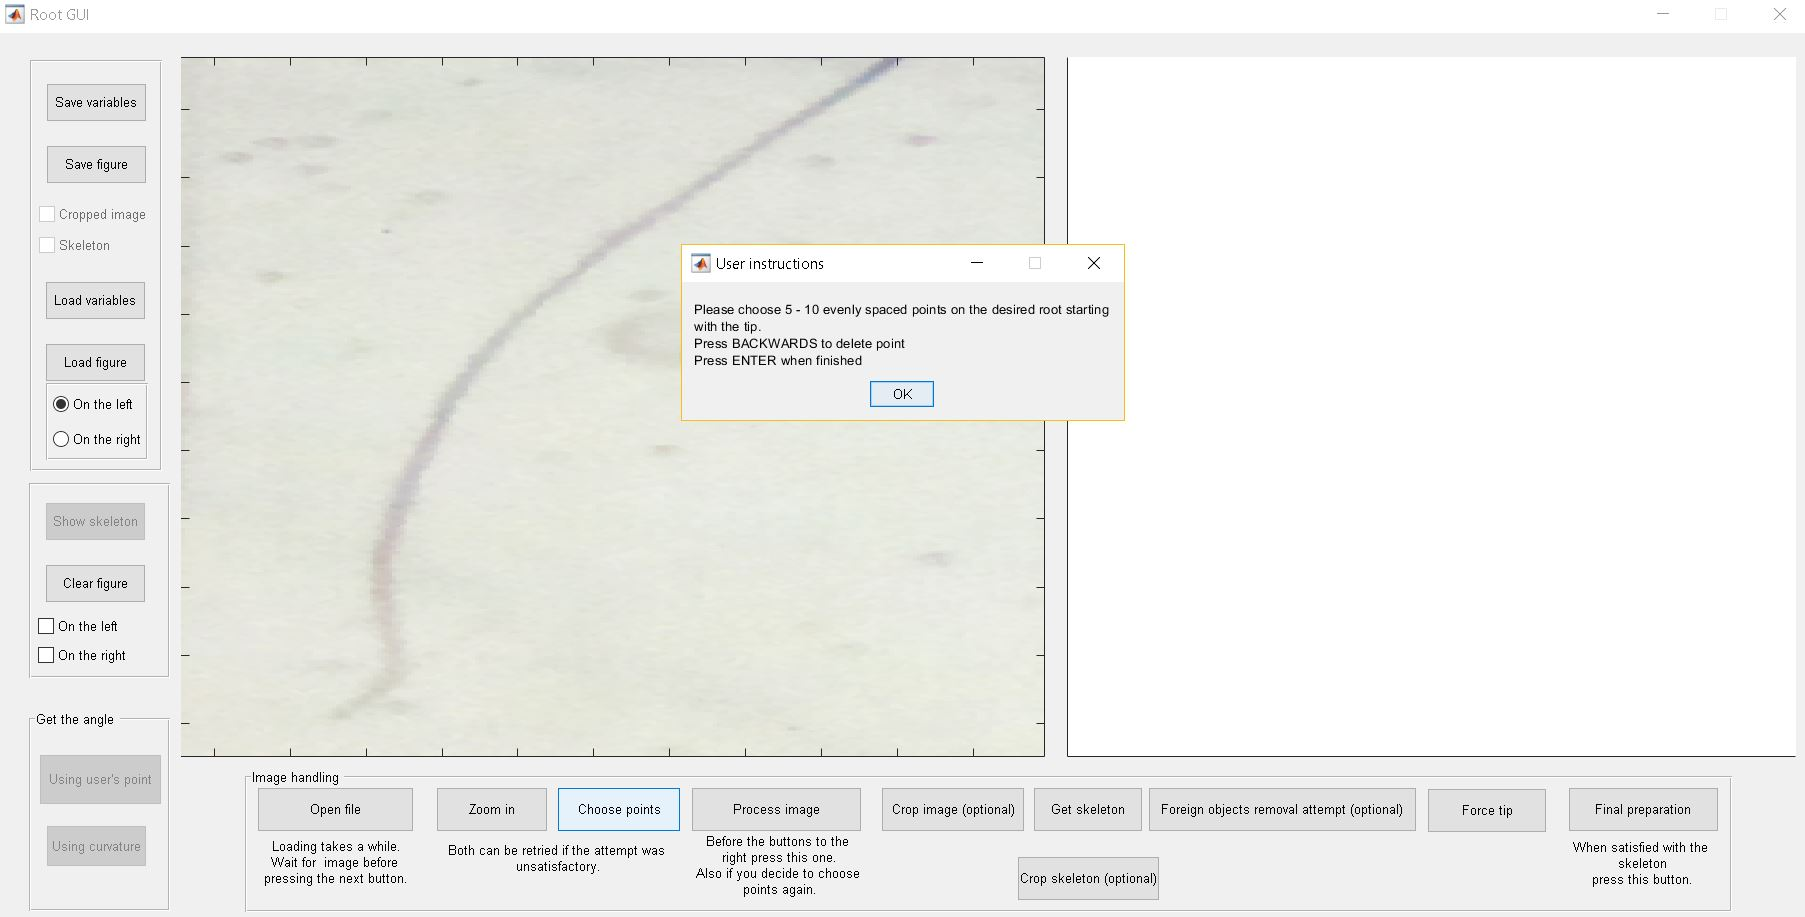
\includegraphics[width=\textwidth]{../Figures/manual/step9.jpg}
	\caption{Prompt to choose 5-10 points on the root starting with the tip}
	\label{fig:img12}
\end{figure}

\begin{figure}[H]
	\centering
	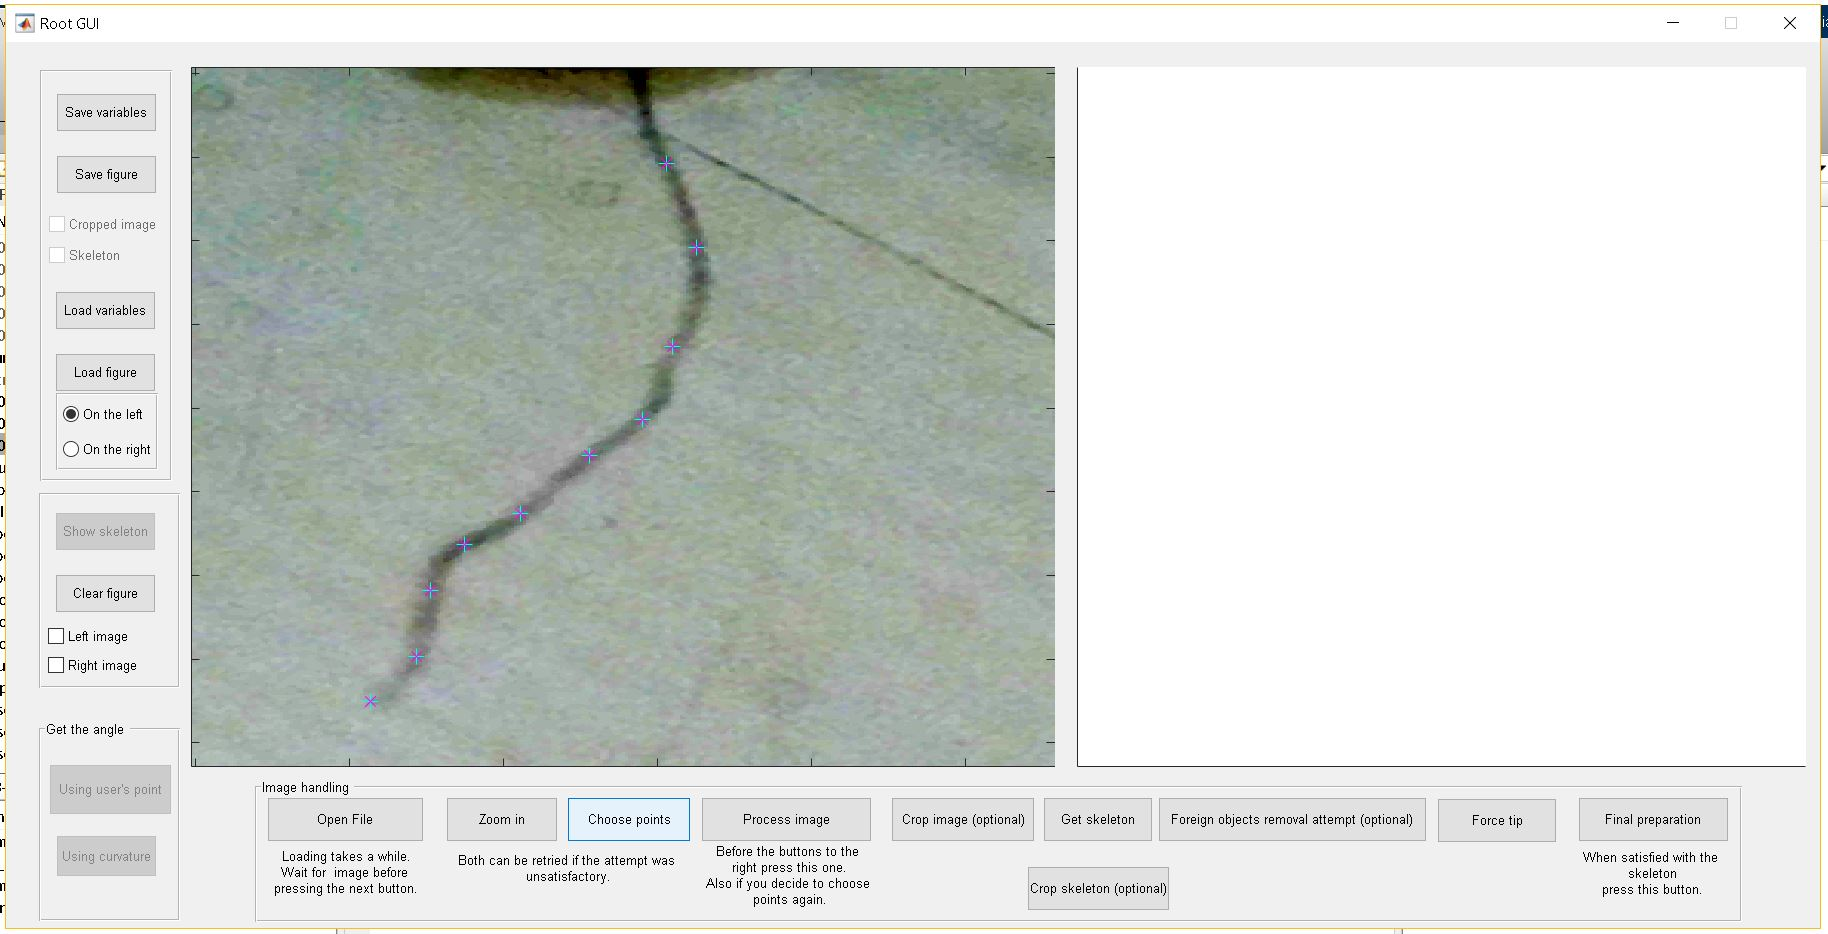
\includegraphics[width=\textwidth]{../Figures/manual/step10.jpg}
	\caption{After choosing the 5-10 points on the root}
	\label{fig:img13}
\end{figure}

\begin{figure}[H]
	\centering
	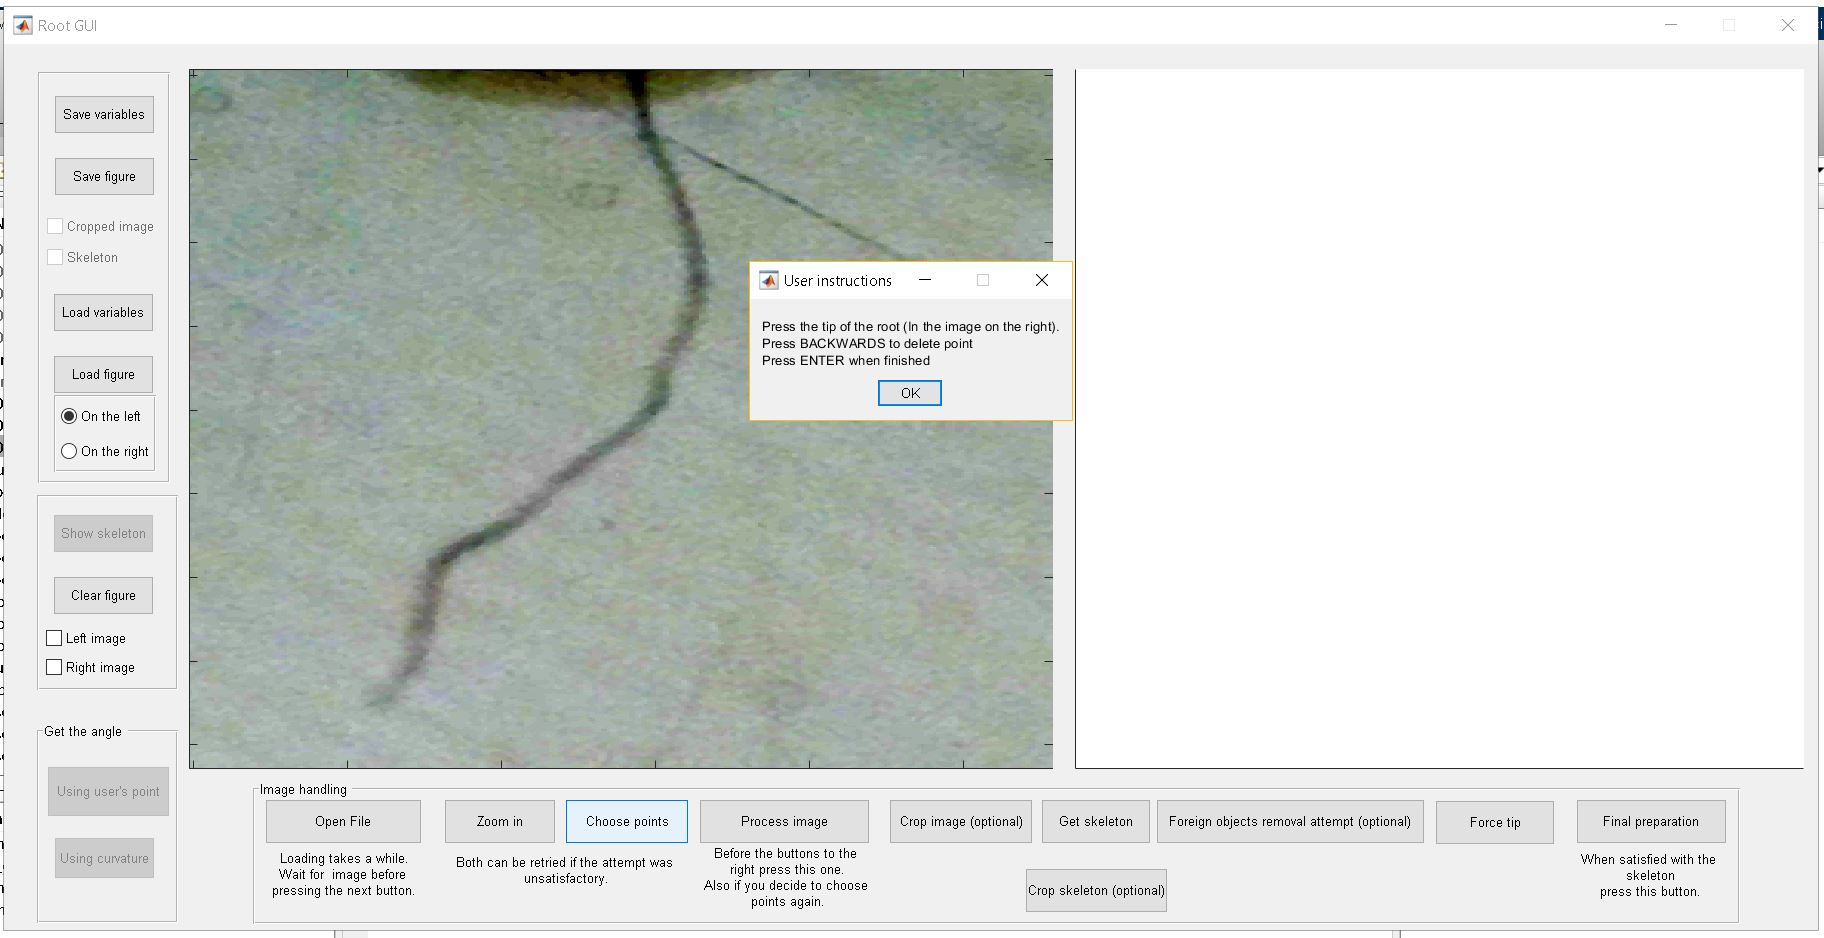
\includegraphics[width=\textwidth]{../Figures/manual/step11.jpg}
	\caption{Prompt to press the tip of the root in the image on the RHS}
	\label{fig:img14}
\end{figure}

\begin{figure}[H]
	\centering
	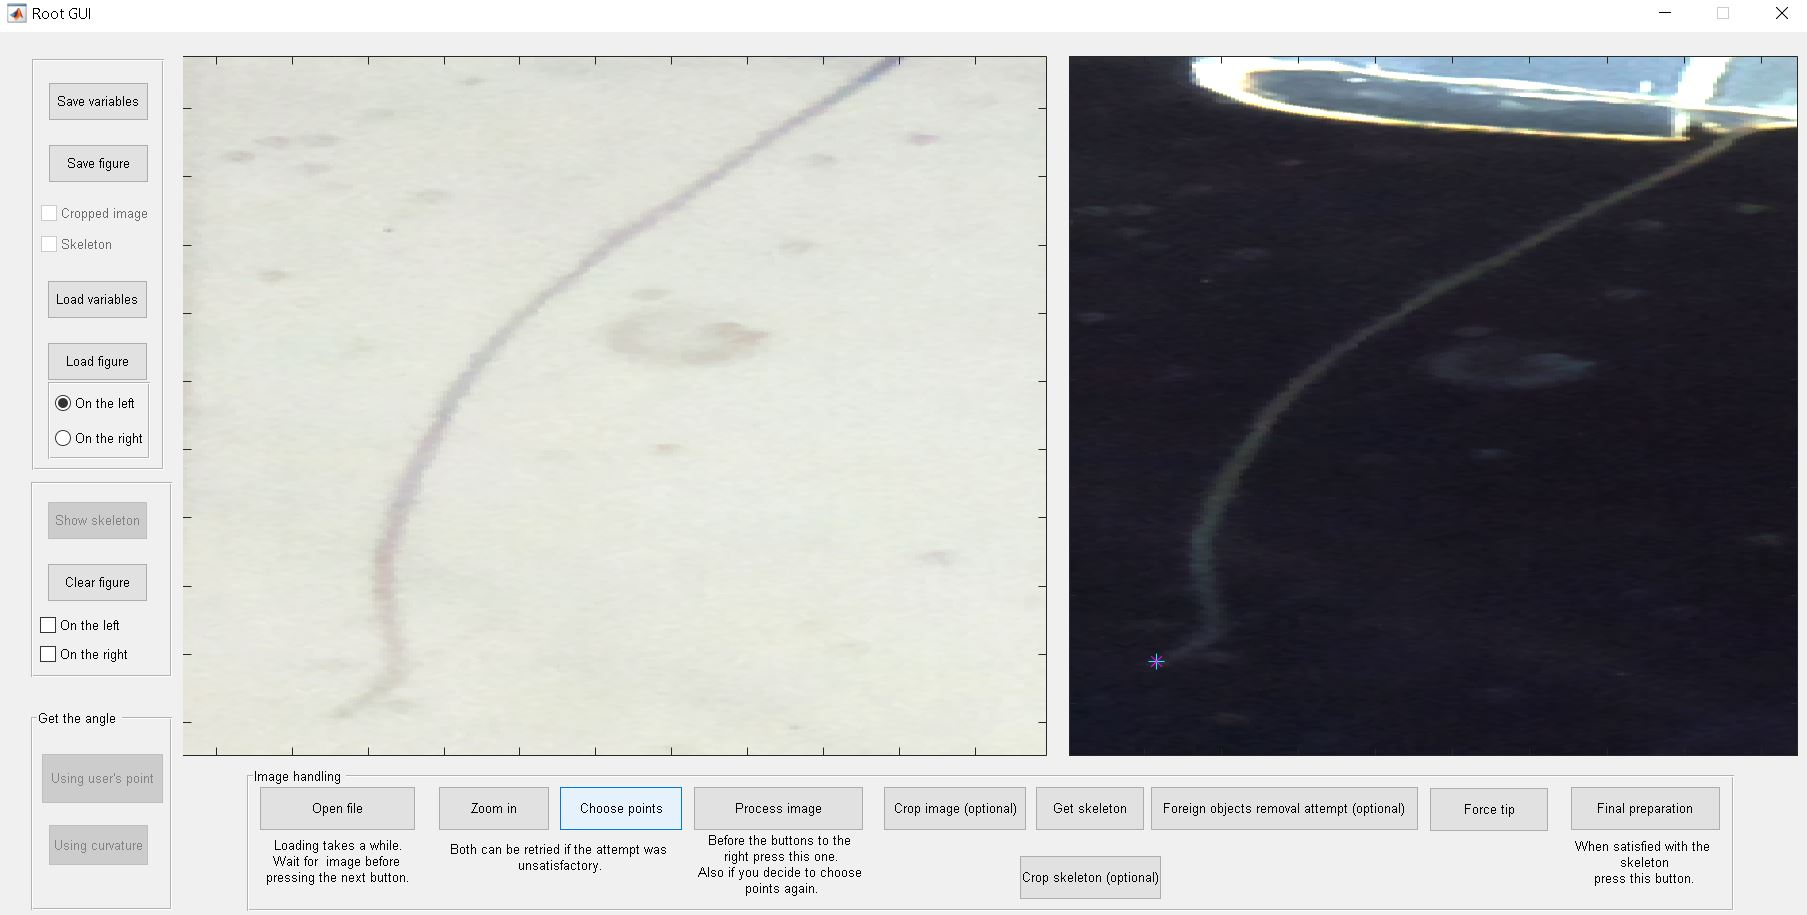
\includegraphics[width=\textwidth]{../Figures/manual/step12.jpg}
	\caption{After choosing the tip of the root}
	\label{fig:img15}
\end{figure}

Now that we did the work to feed in some points, it's time to let the program do its part. Click on the \textit{Process image} buton to make the program preprocess the image for the next part of getting the skeleton (see figure \ref{fig:img16}).

\begin{figure}[H]
	\centering
	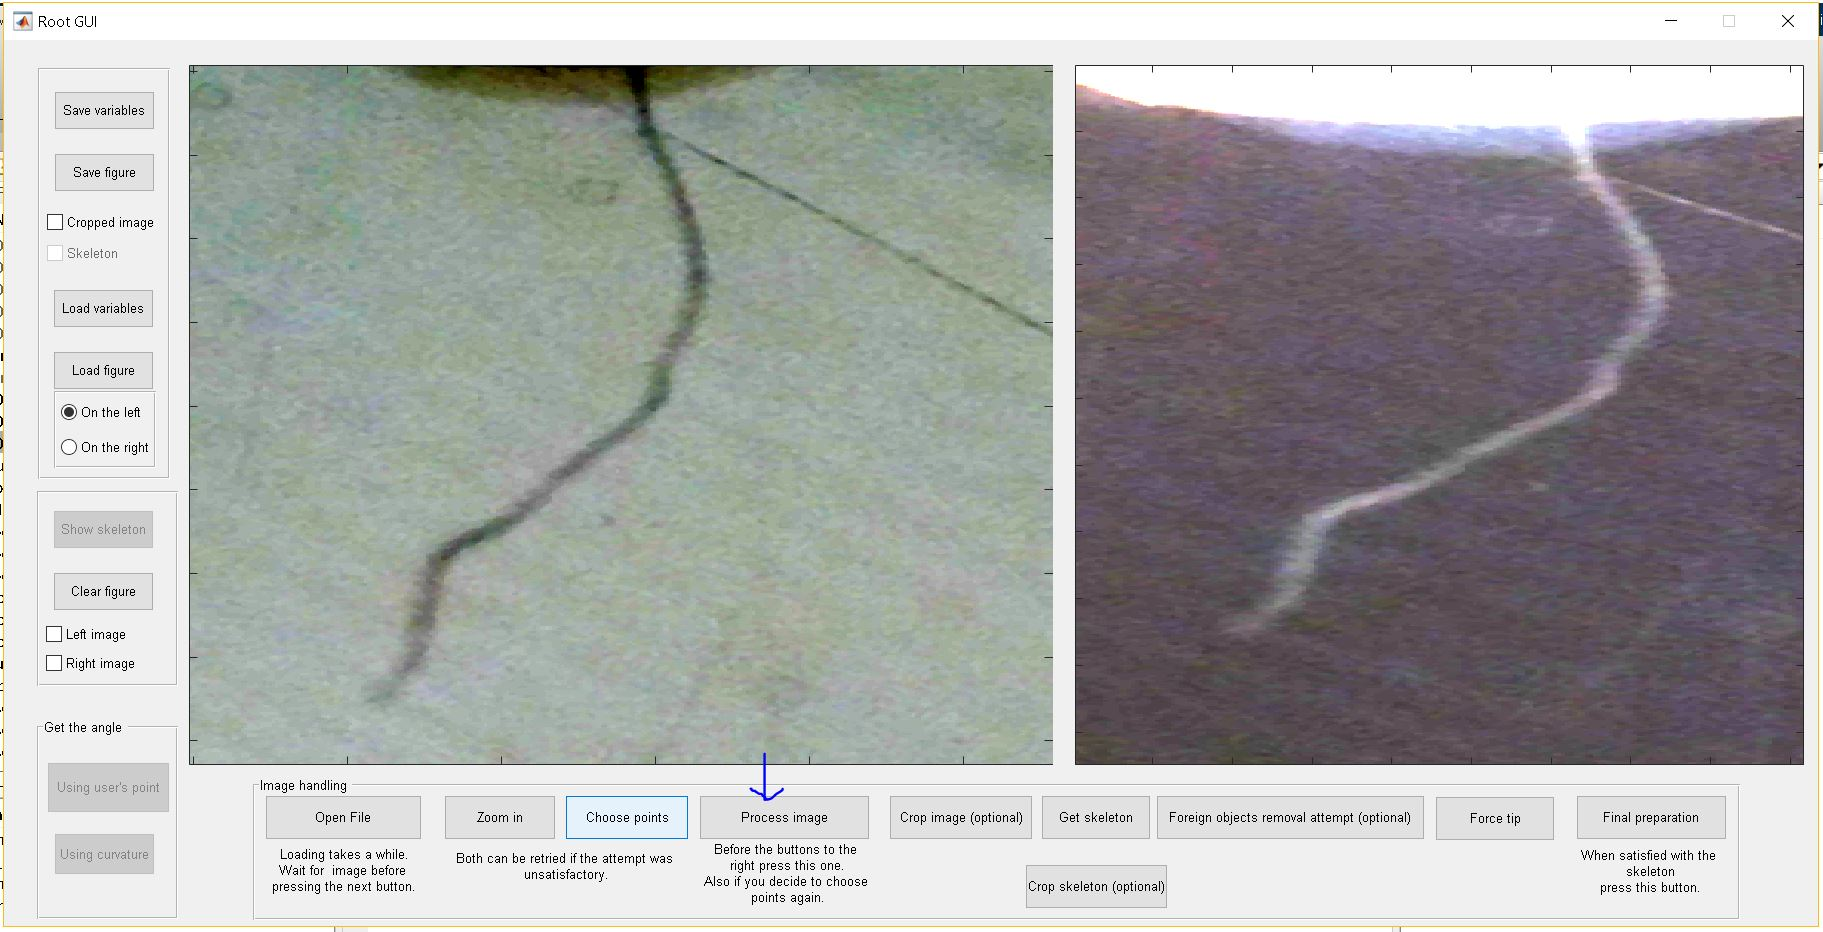
\includegraphics[width=\textwidth]{../Figures/manual/step13.jpg}
	\caption{Step 4 in the \textit{RootSkel} pipeline: Processing the image}
	\label{fig:img16}
\end{figure}

A message will pop up when the processing is done (see figure \ref{fig:img17}).
\begin{figure}[H]
	\centering
	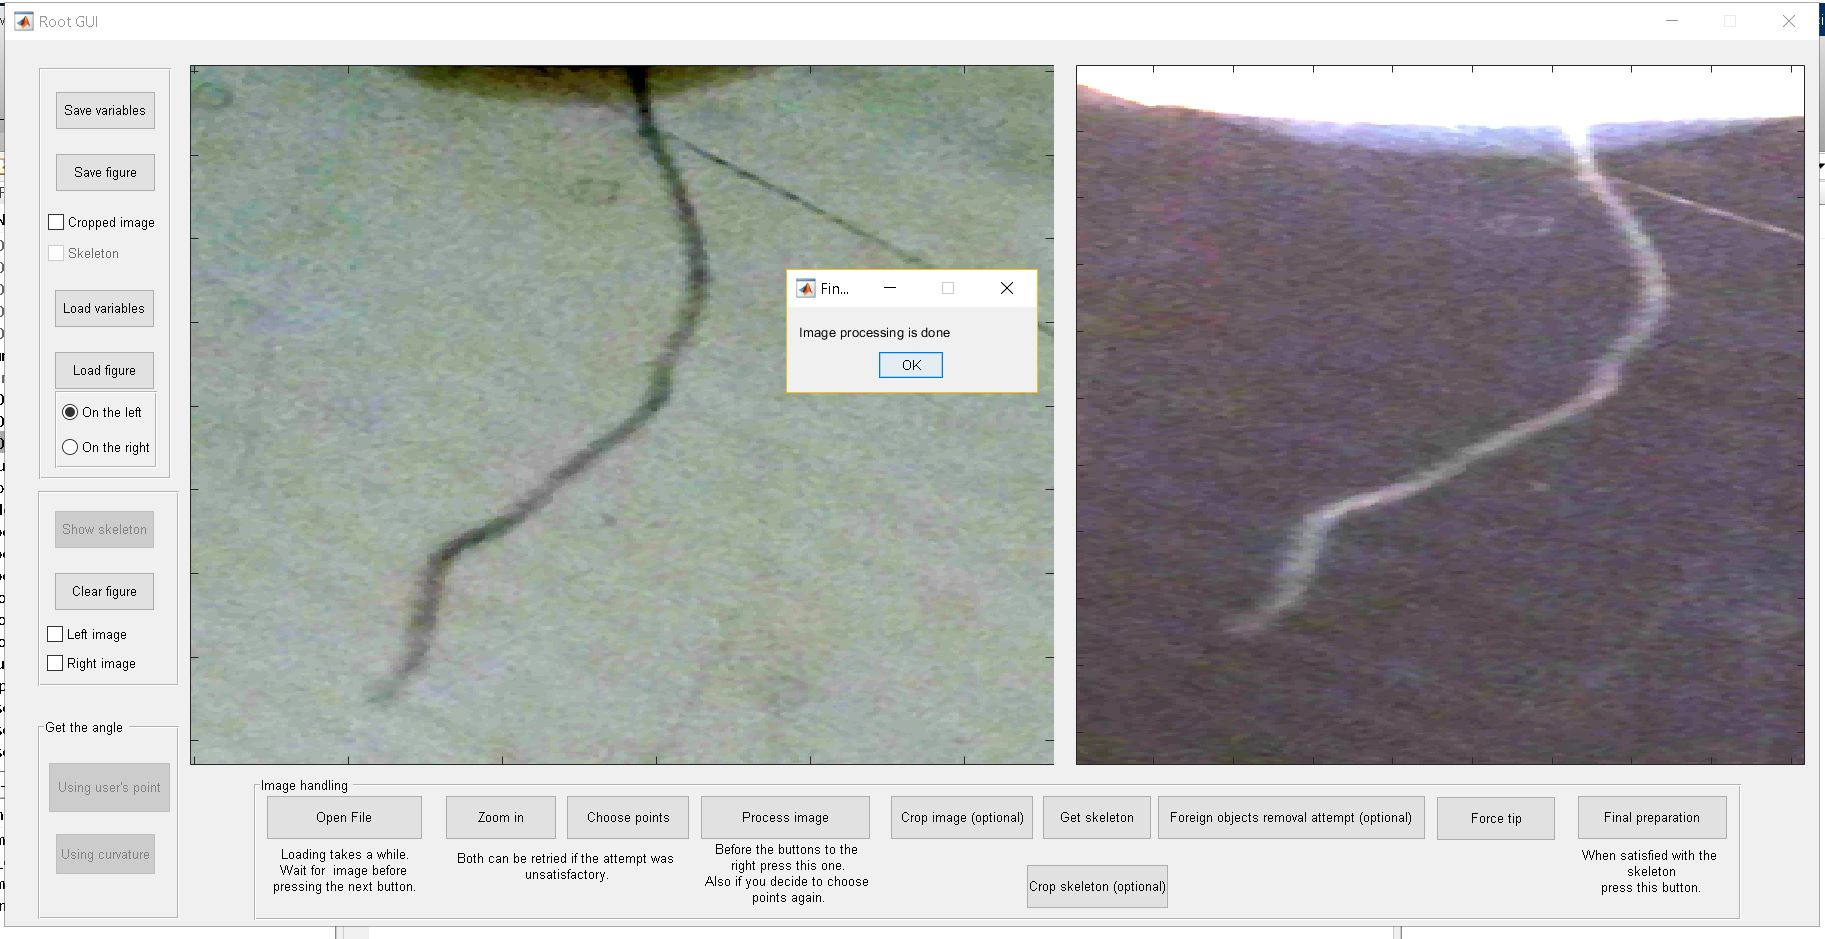
\includegraphics[width=\textwidth]{../Figures/manual/step14.jpg}
	\caption{After the processing is done}
	\label{fig:img17}
\end{figure}

Now we need to click the \textit{Get skeleton} button (see figure \ref{fig:img18}) to get the result in the image on the RHS (see figure \ref{fig:img19}).

\begin{figure}[H]
	\centering
	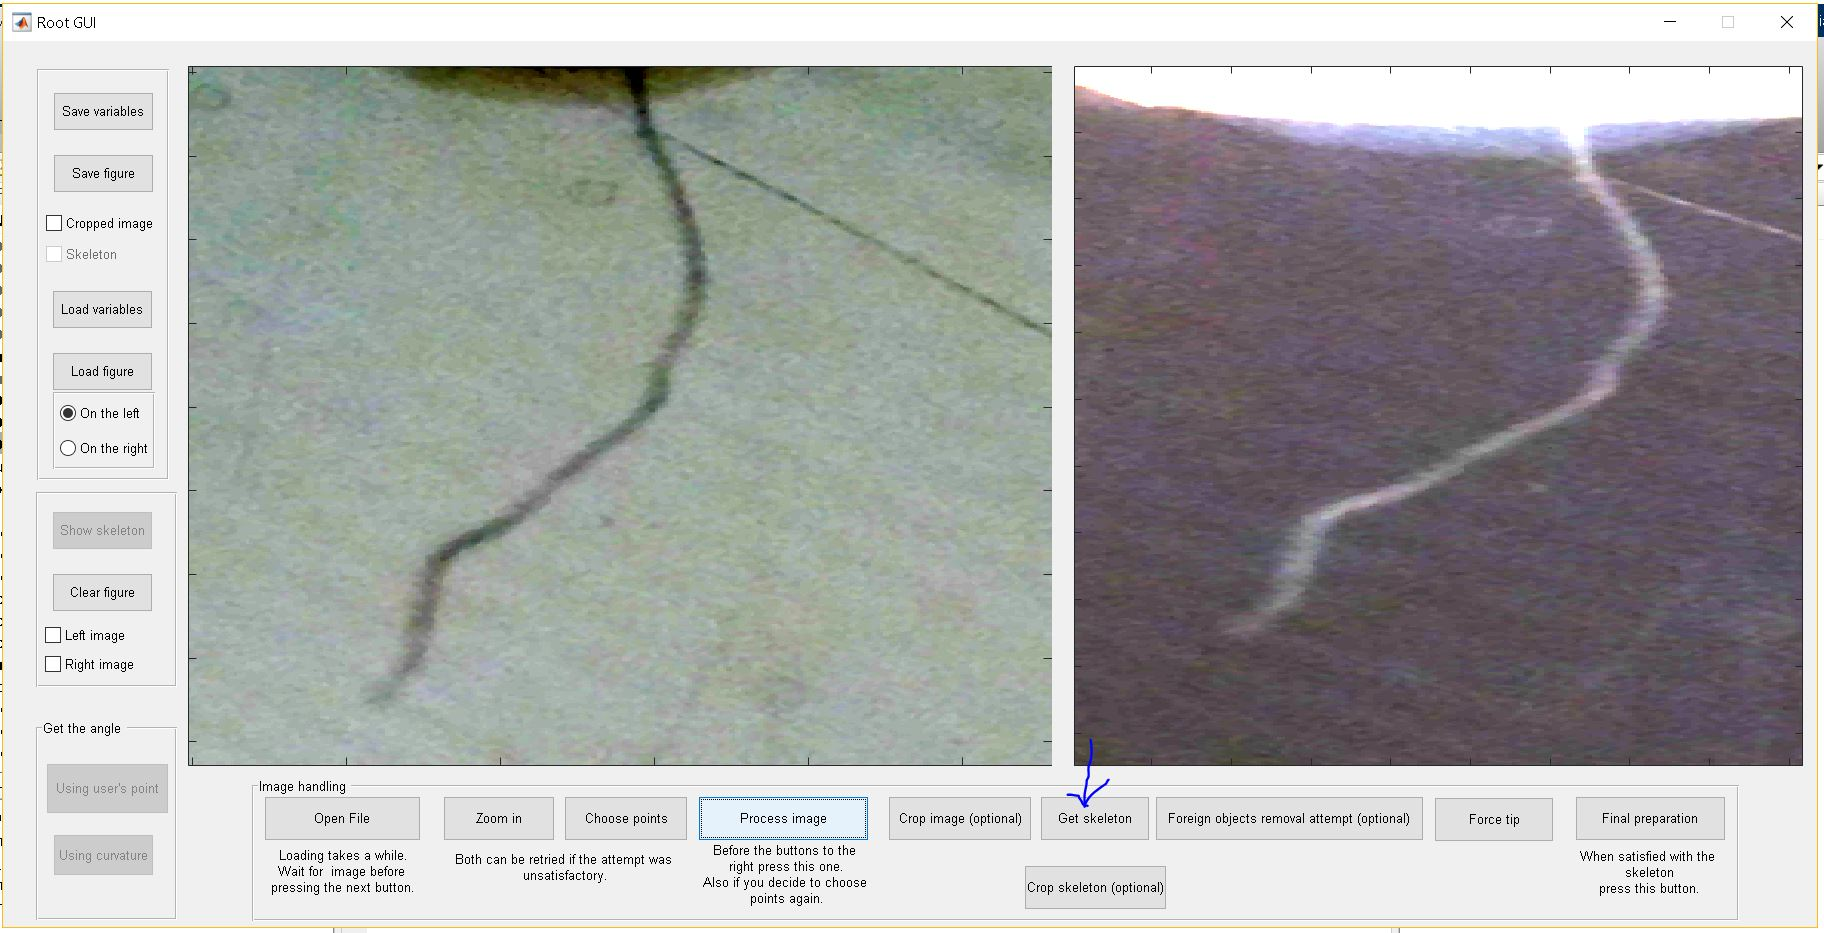
\includegraphics[width=\textwidth]{../Figures/manual/step15.jpg}
	\caption{Step 5 in the \textit{RootSkel} pipeline: Getting the skeleton}
	\label{fig:img18}
\end{figure}

\begin{figure}[H]
	\centering
	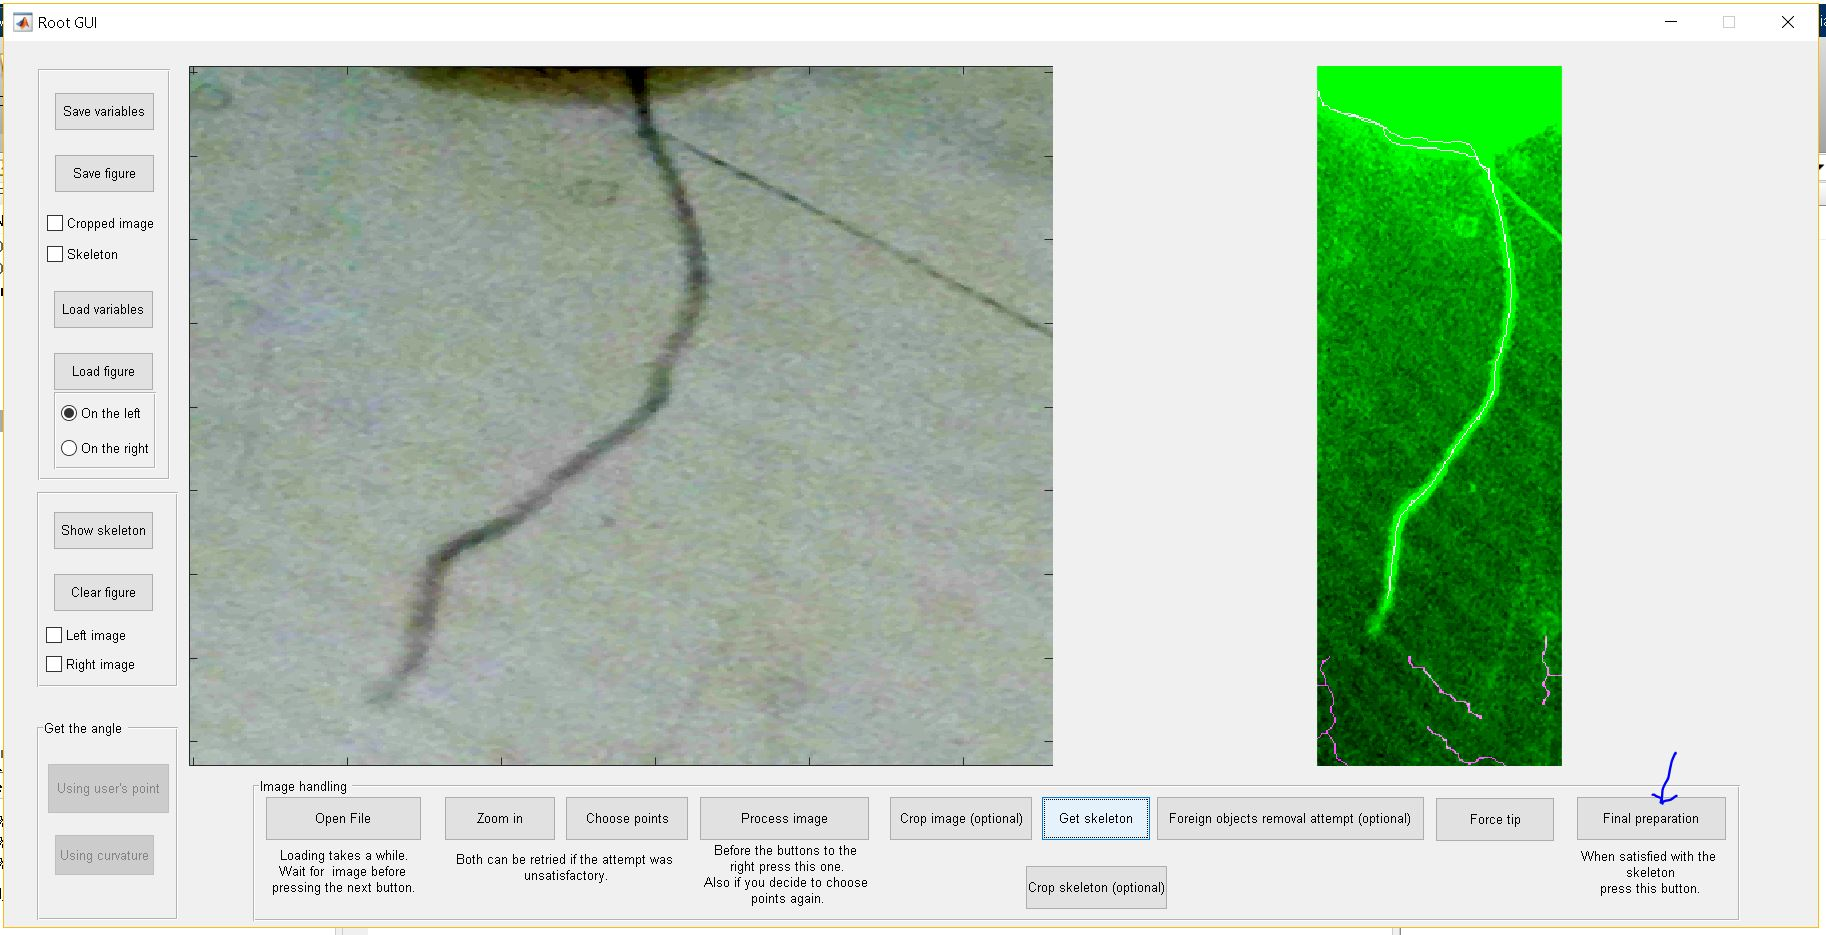
\includegraphics[width=\textwidth]{../Figures/manual/step16.jpg}
	\caption{Getting the skeleton}
	\label{fig:img19}
\end{figure}

Now we've got ourselves a root (it's not perfect, but we'll get into optional improvement steps in a minute), so it's time to get on with it. 
Let's now click the \textit{Final preparation} button and then click 'No' when presented the chance (we will get into the alternative option later) to get ready for the angle calculation (see figures \ref{fig:img19} and \ref{fig:img20}).

\begin{figure}[H]
	\centering
	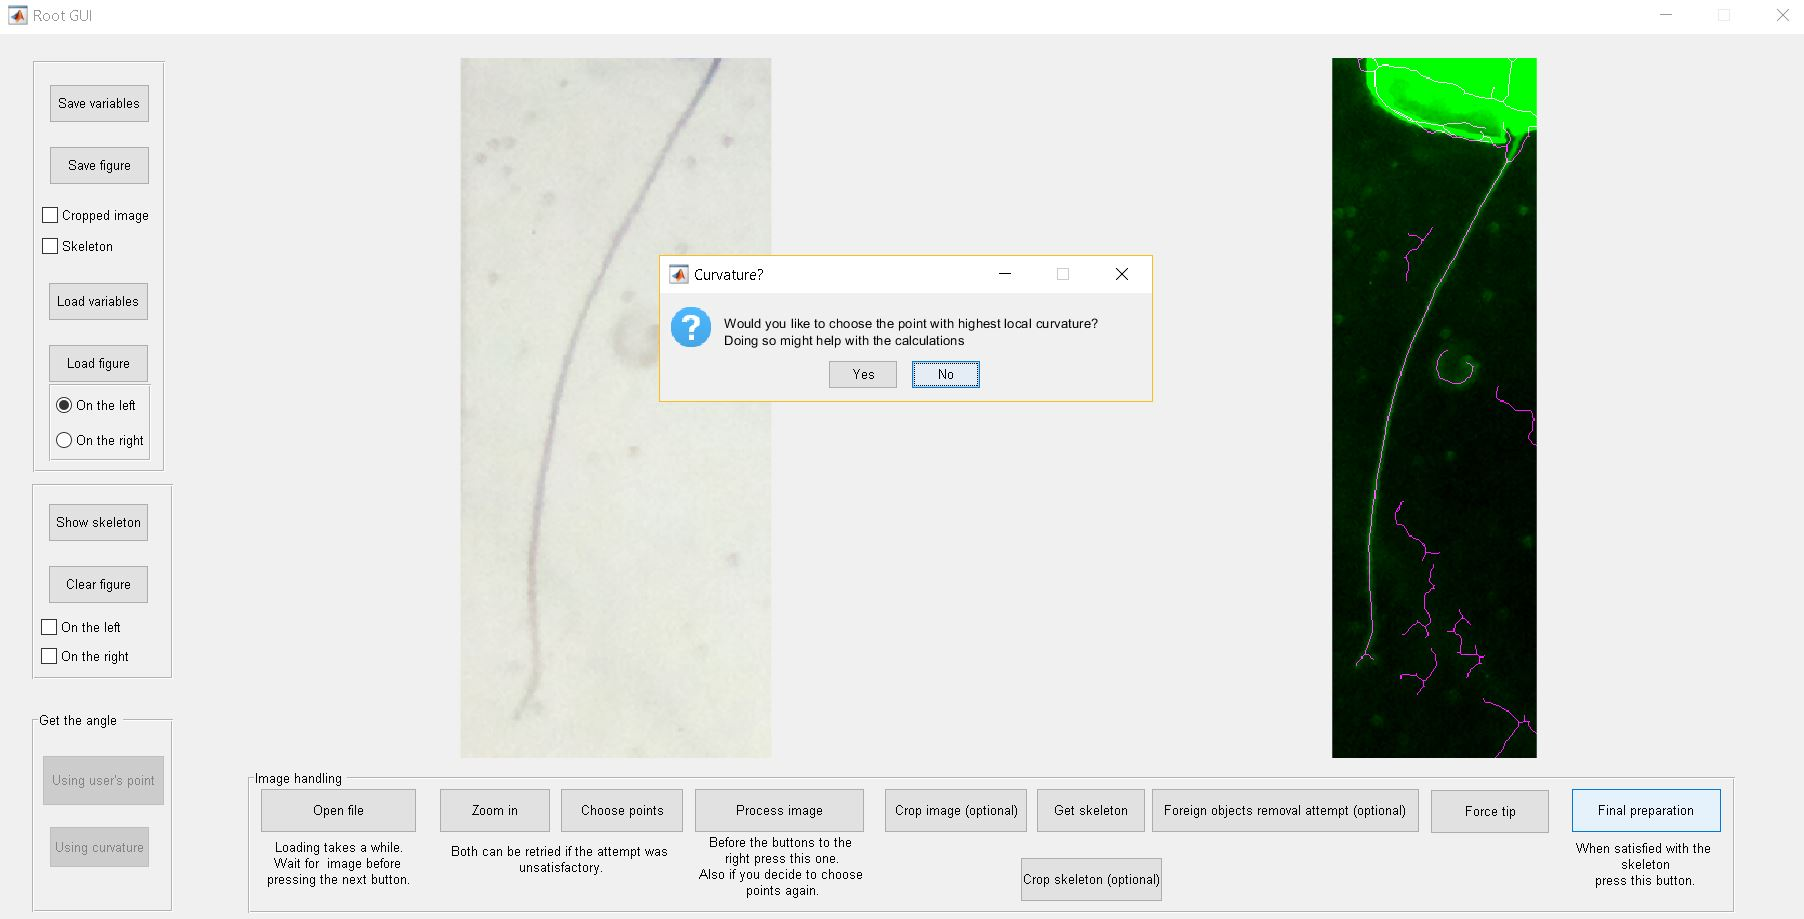
\includegraphics[width=\textwidth]{../Figures/manual/step17.jpg}
	\caption{Clicking 'No' when asked to choose the point of highest local (mean) curvature}
	\label{fig:img20}
\end{figure}

Here we are, the last step before we get an angle for our root. 
All that is left to do, is clicking one of the angle calculations buttons.
Now, since we clicked 'No' in the previous step, we only get the \textit{Using curvature} button, so click this one (see figure \ref{fig:img21}).
Later in the manual, we will go over the option to include a point of local maximum curvature by the user. 
Now you will get the angle and then you will be asked to enter the root number (unless you clicked on one of the other buttons requiring this information, i.e. \textit{Save variables} and \textit{Save figures}. More on that later.) (see figures \ref{fig:img22} and \ref{fig:img23}).

\begin{figure}[H]
	\centering
	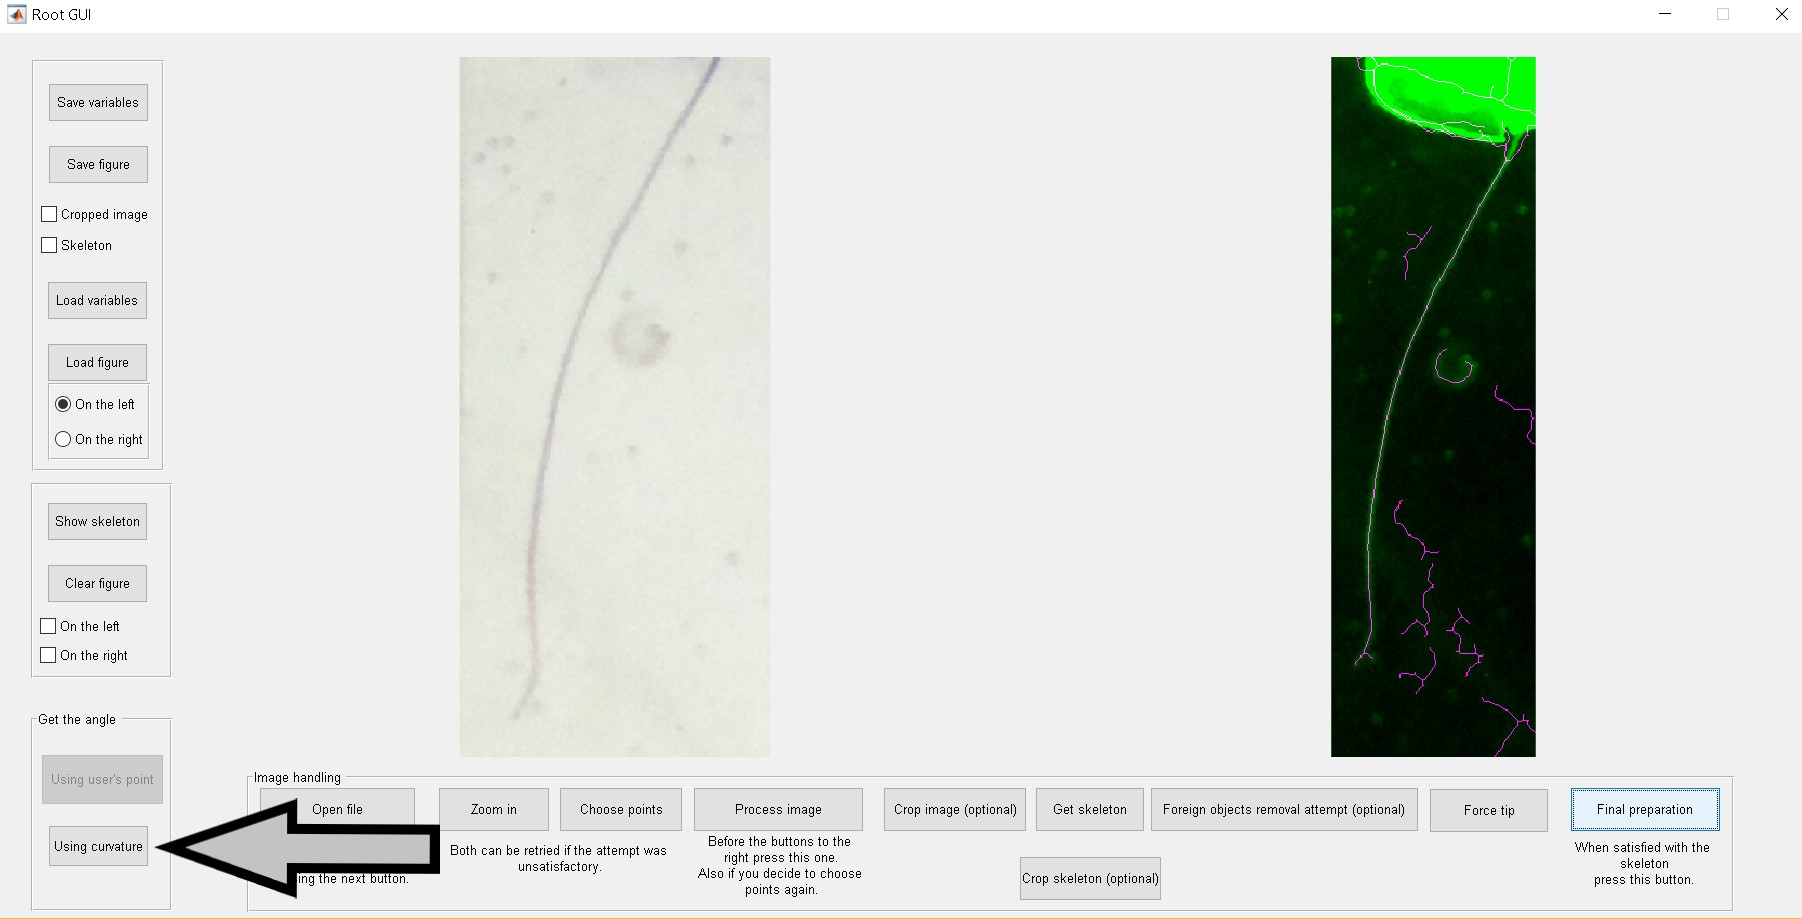
\includegraphics[width=\textwidth]{../Figures/manual/step18.jpg}
	\caption{Step 6 in the \textit{RootSkel} pipeline: Clicking \textit{Using curvature} for the angle computation}
	\label{fig:img21}
\end{figure}

\begin{figure}[H]
	\centering
	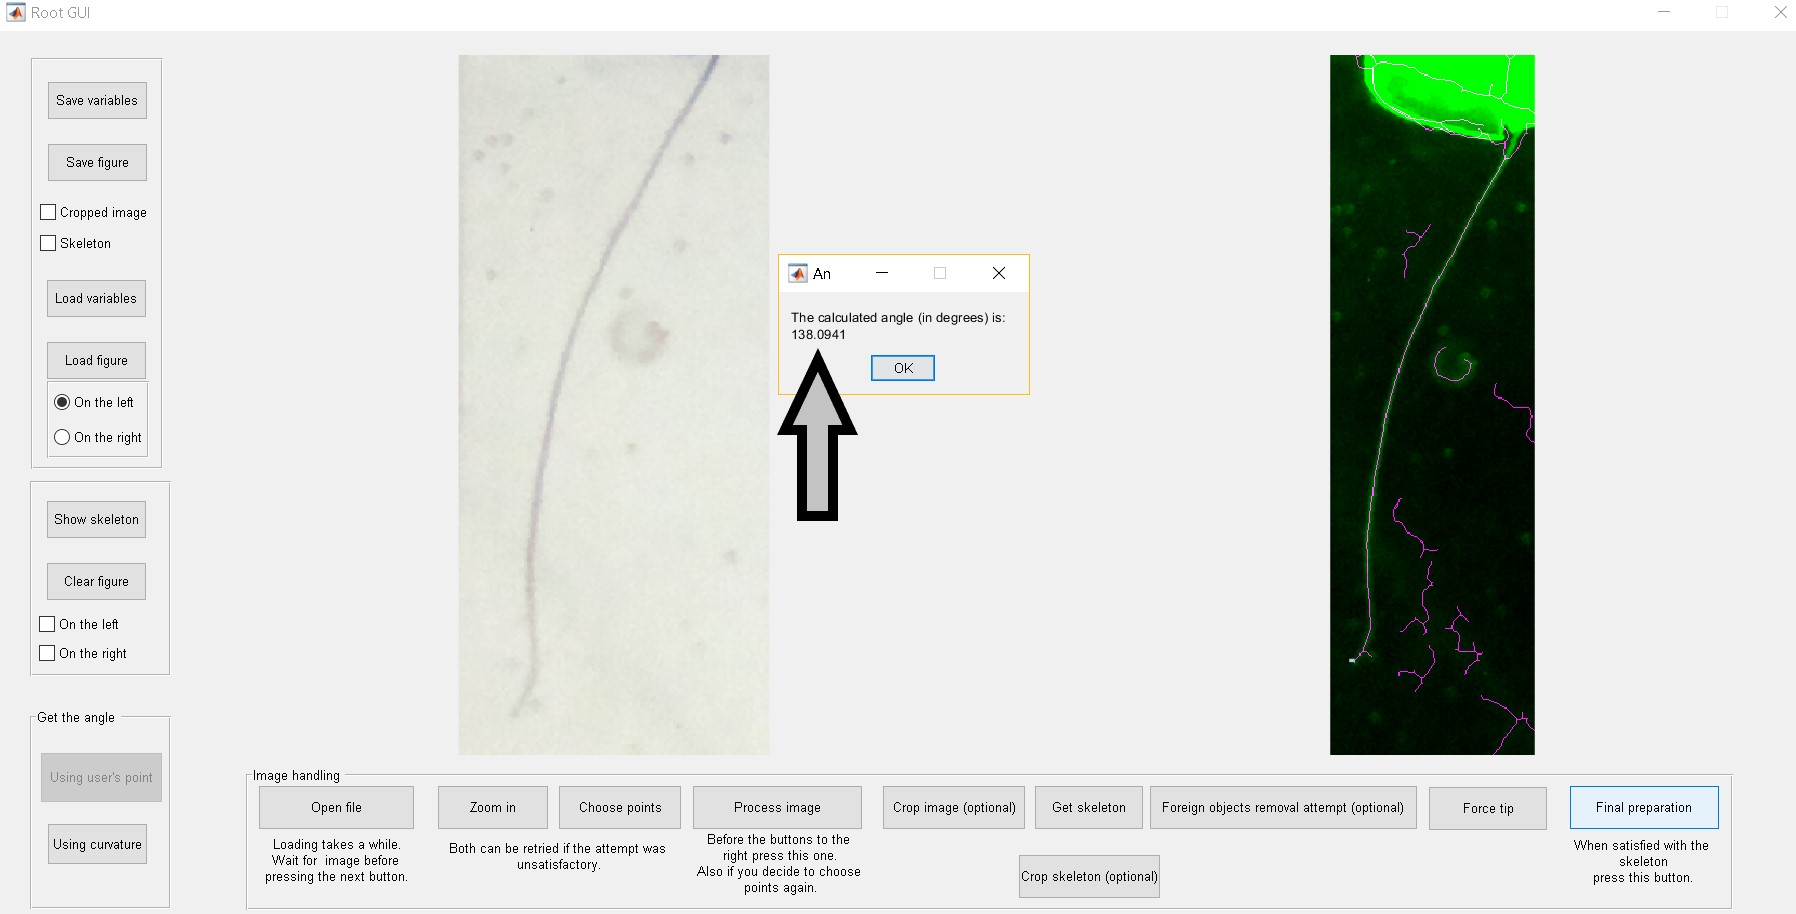
\includegraphics[width=\textwidth]{../Figures/manual/step19.jpg}
	\caption{Getting the computed the angle}
	\label{fig:img22}
\end{figure}

\begin{figure}[H]
	\centering
	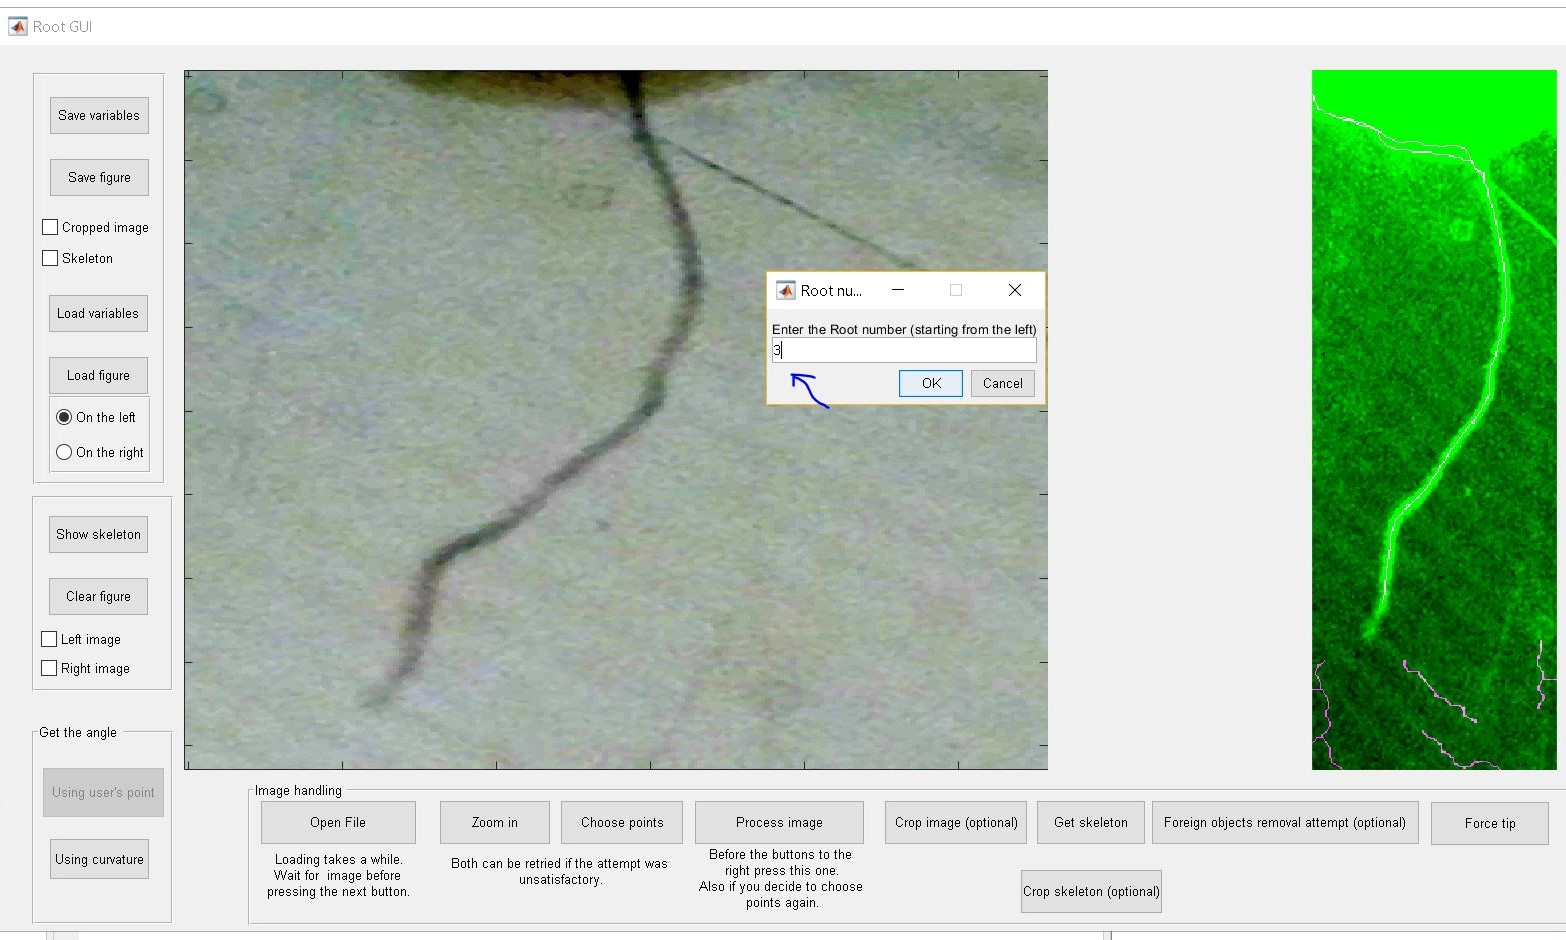
\includegraphics[width=\textwidth]{../Figures/manual/step20.jpg}
	\caption{Entering the root number (starting from the LHS)}
	\label{fig:img23}
\end{figure}

And that's it. At least without any optional steps. To the optional features we will get later in the manual. 


%----------------------------------------------------------------------------------------
\subsection{Saving}

Now say you want to save the data you got after the \textit{Final preparation}. That's what the save buttons are for.
We'll start with \textit{Save variables} (see figure \ref{fig:img24}).

\begin{figure}[H]
	\centering
	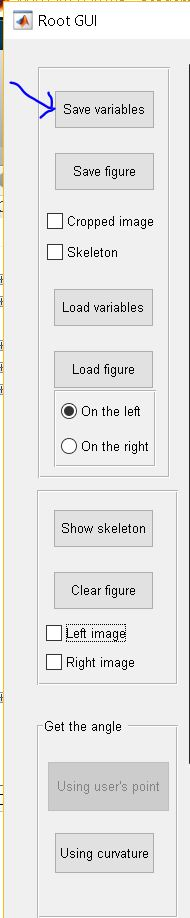
\includegraphics[width=0.3\textwidth]{../Figures/manual/save1.jpg}
	\caption{Saving all relevant variables}
	\label{fig:img24} 
\end{figure}

After you have clicked the \textit{Save variables} button, you will be prompted to give the program the root number if you haven't done so yet (see figure \ref{fig:img23}).
Otherwise you will see the following on your screen:

\begin{figure}[H]
	\centering
	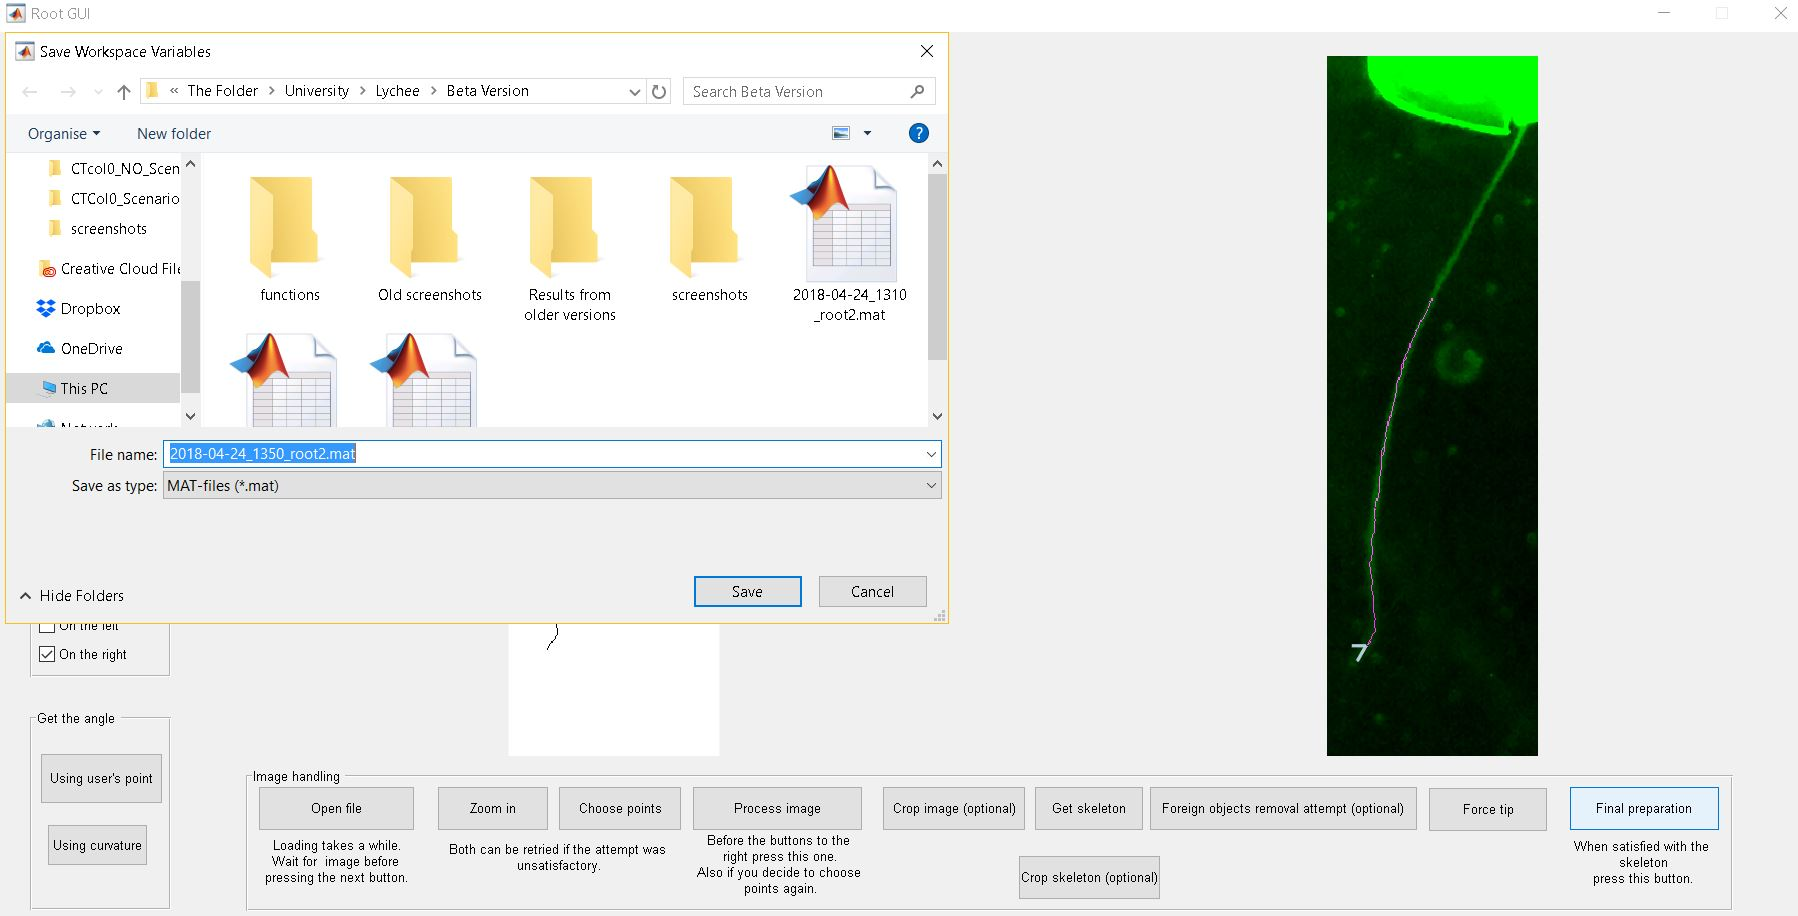
\includegraphics[width=\textwidth]{../Figures/manual/save2.jpg}
	\caption{Saving the relevant variables in a .mat file}
	\label{fig:img25}
\end{figure}

As you can see, the default name consists of the name of the original image file and the number of the root. 
So now you can save your root data in a .mat file whenever you want. You will see the .mat folder in the specified location on the LHS on the screen (see figure \ref{fig:img26}).

\begin{figure}[H]
	\centering
	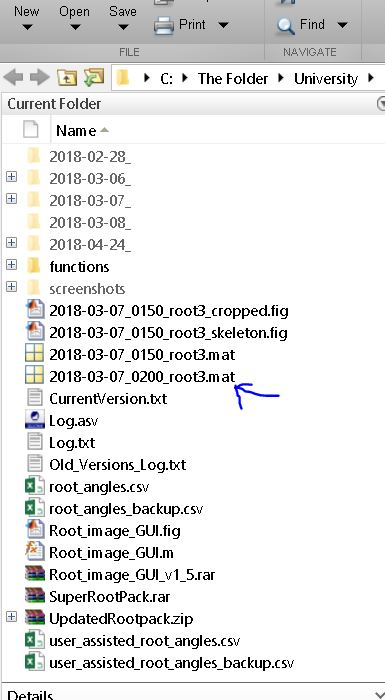
\includegraphics[width=0.5\textwidth]{../Figures/manual/save3.jpg}
	\caption{The saved .mat file with the relevant variables popping up on the LHS of the MATLAB GUI}
	\label{fig:img26}
\end{figure}

Now that we saved the variables, let's talk about saving figures. As you can see in figure \ref{fig:img27} two figures can be saved: One focused on the root, called \textit{Cropped image} (the figure on the RHS in figures \ref{fig:img15} -- \ref{fig:img18}), and the other one is the skeleton overlayed on the root, called \textit{Skeleton} (the figure on the RHS in figures \ref{fig:img19} -- \ref{fig:img23}).
You can choose to save either one of them or both.

Assume we clicked both.

\begin{figure}[H]
	\centering
	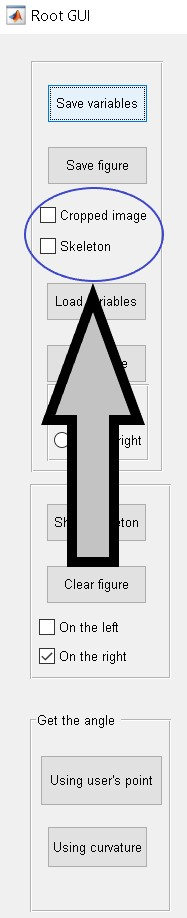
\includegraphics[width=0.3\textwidth]{../Figures/manual/save4.jpg}
	\caption{Saving of different figures: the cropped image or the skeleton}
	\label{fig:img27}
\end{figure}

Now that both are selected, the next step is to simply click on \textit{Save figure}(see figure \ref{fig:img28}).

\begin{figure}[H]
	\centering
	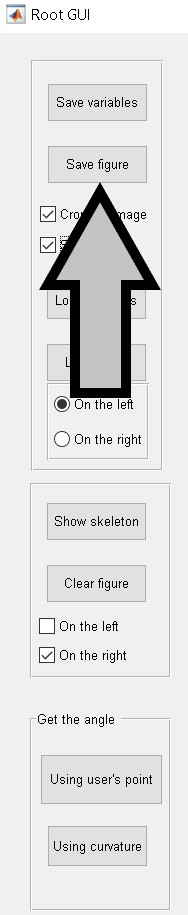
\includegraphics[width=0.3\textwidth]{../Figures/manual/save5.jpg}
	\caption{Clicking the \textit{Save figure} button}
	\label{fig:img28}
\end{figure}

After that's done, two new .fig files will appear with the appropriate end to their file name (see figure \ref{fig:img29}).

\begin{figure}[H]
	\centering
	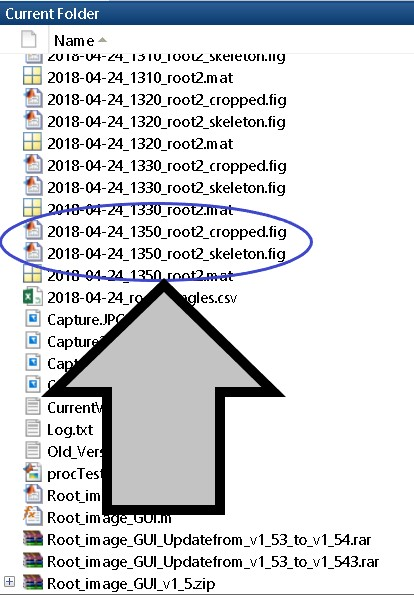
\includegraphics[width=0.6\textwidth]{../Figures/manual/save6.jpg}
	\caption{The saved .fig file(s) appearing on the LHS of the MATLAB GUI}
	\label{fig:img29}
\end{figure}


%----------------------------------------------------------------------------------------
\subsection{Optional}

Alright, now let's get into optional things you might try to improve the skeleton.

\subsubsection{Foreign objects removal}

First, there is a \textit{Foreign object removal} attempt, an additional cleaning step (see figure \ref{fig:img30}):

\begin{figure}[H]
	\centering
	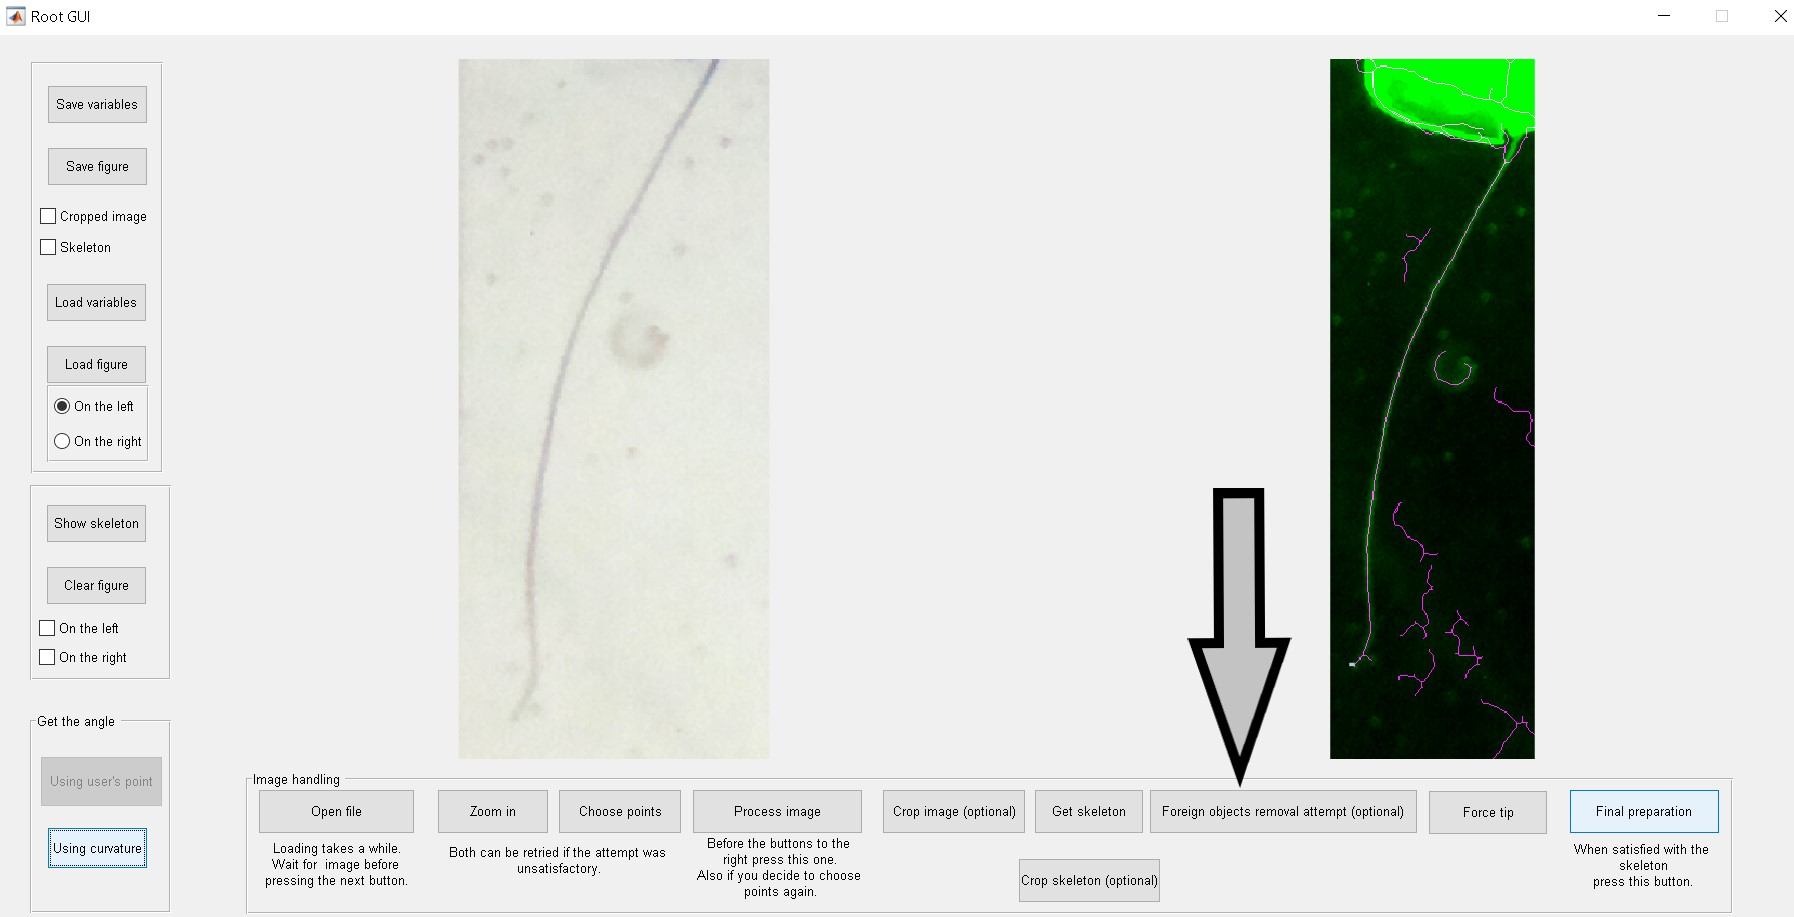
\includegraphics[width=\textwidth]{../Figures/manual/optionalA1.jpg}
	\caption{Optional step in the \textit{RootSkel} pipeline: Foreing objects removal}
	\label{fig:img30}
\end{figure}

Next you will see a message box with instructions. The basic thing is, the more times you press 'Yes' after that (see figure \ref{fig:img32}), the bigger the objects the program will try to remove.
So you can press 'Yes' as many times as you need until the foreign objects are dealt with as they are in figure \ref{fig:img32}.

\begin{figure}[H]
	\centering
	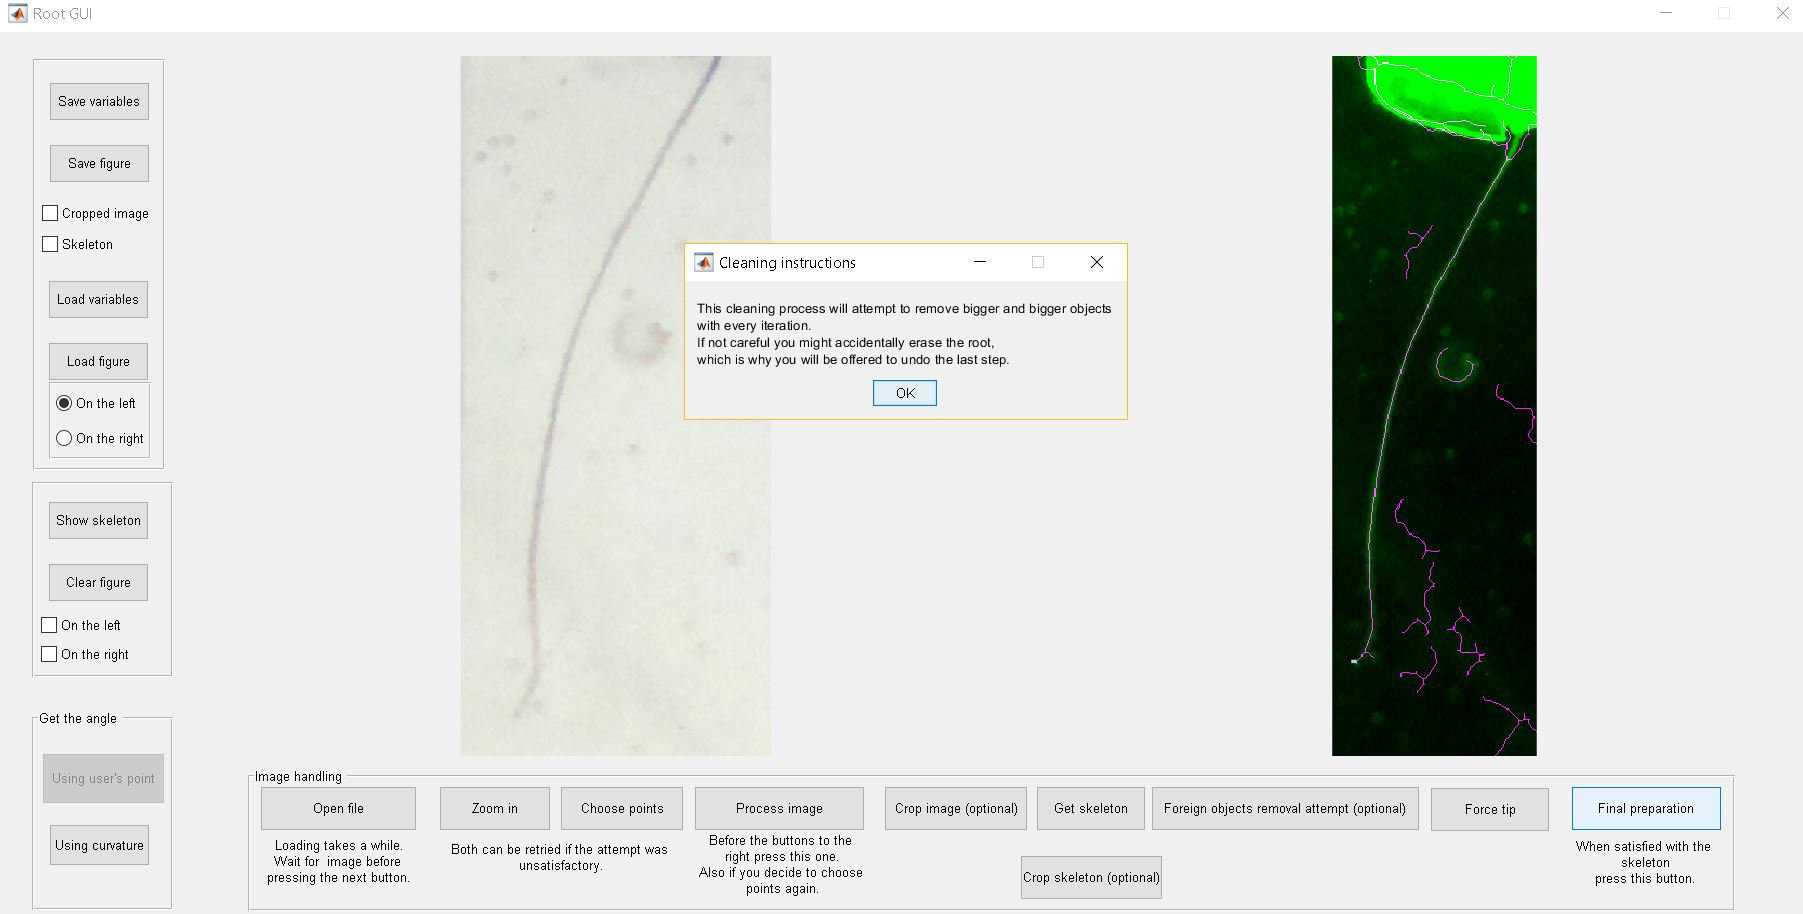
\includegraphics[width=\textwidth]{../Figures/manual/optionalA2.jpg}
	\caption{Explanation and instruction of the foreign objects removal step}
	\label{fig:img31}
\end{figure}

\begin{figure}[H]
	\centering
	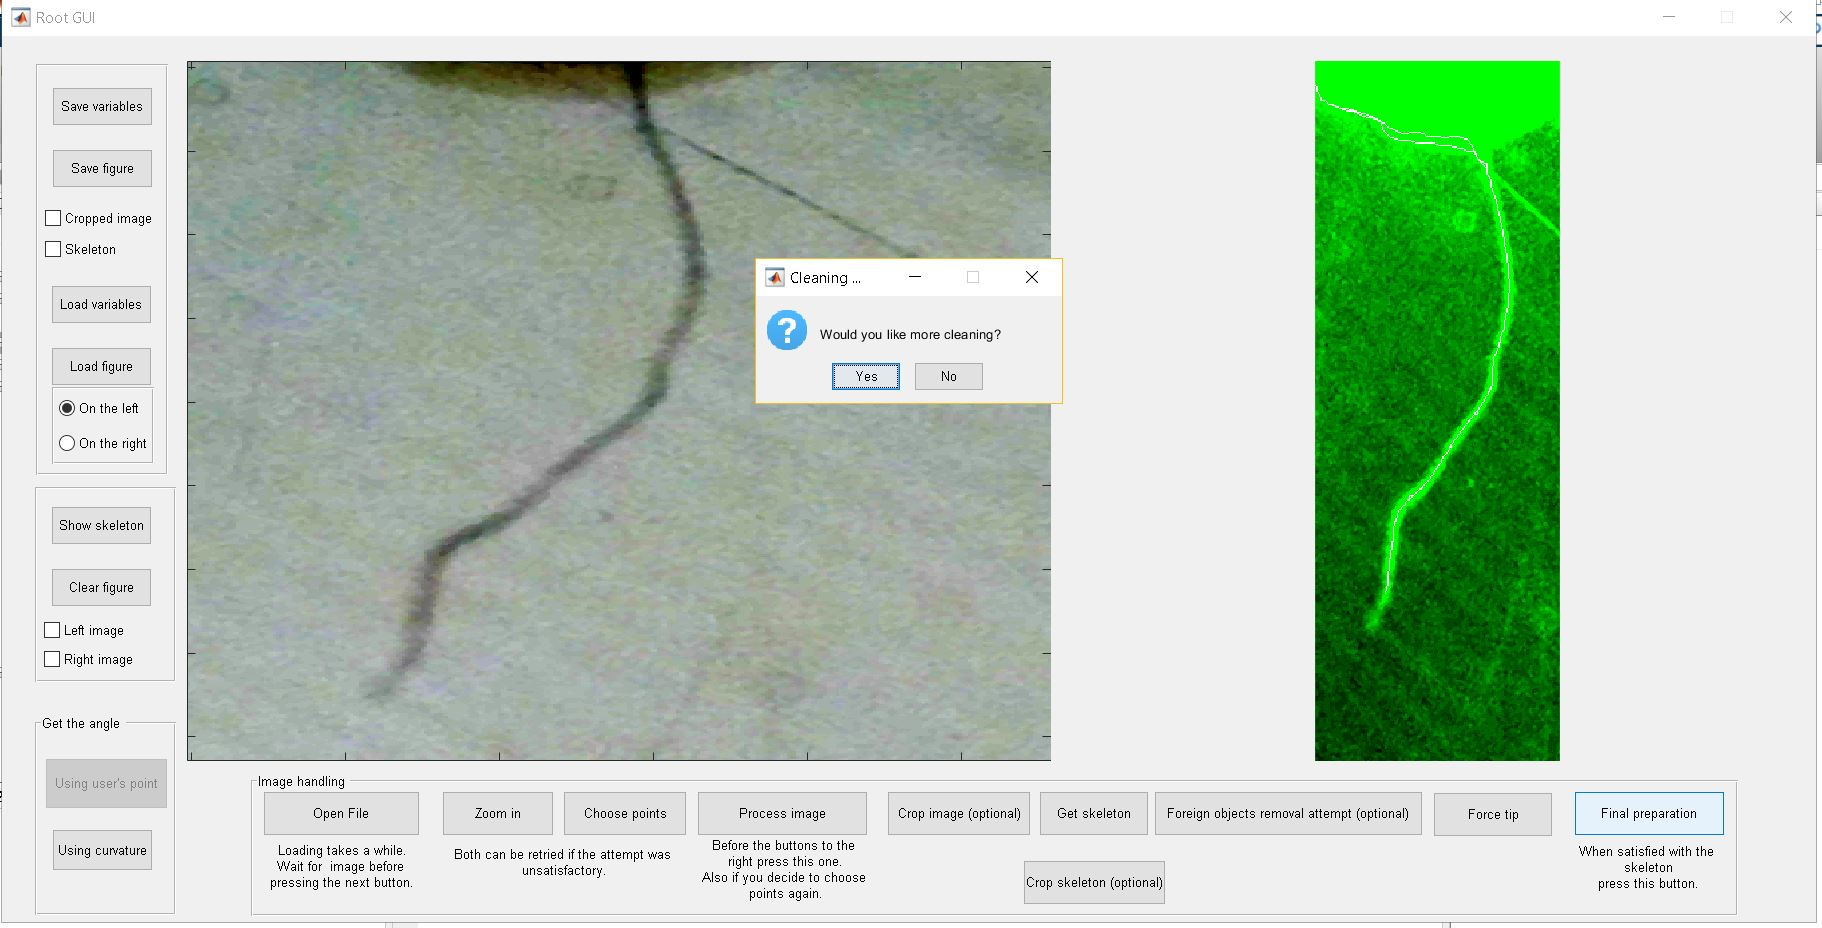
\includegraphics[width=\textwidth]{../Figures/manual/optionalA3.jpg}
	\caption{Prompt for further cleaning}
	\label{fig:img32}
\end{figure}

But what if you pressed 'Yes' once too often and the program deleted the skeleton, as it is in figure \ref{fig:img33}? 
Don't worry! There is an option to undo the last step. 
Just press 'No' and then you will be asked if you want to undo the last step (see figures \ref{fig:img34} -- \ref{fig:img35}).

\begin{figure}[H]
	\centering
	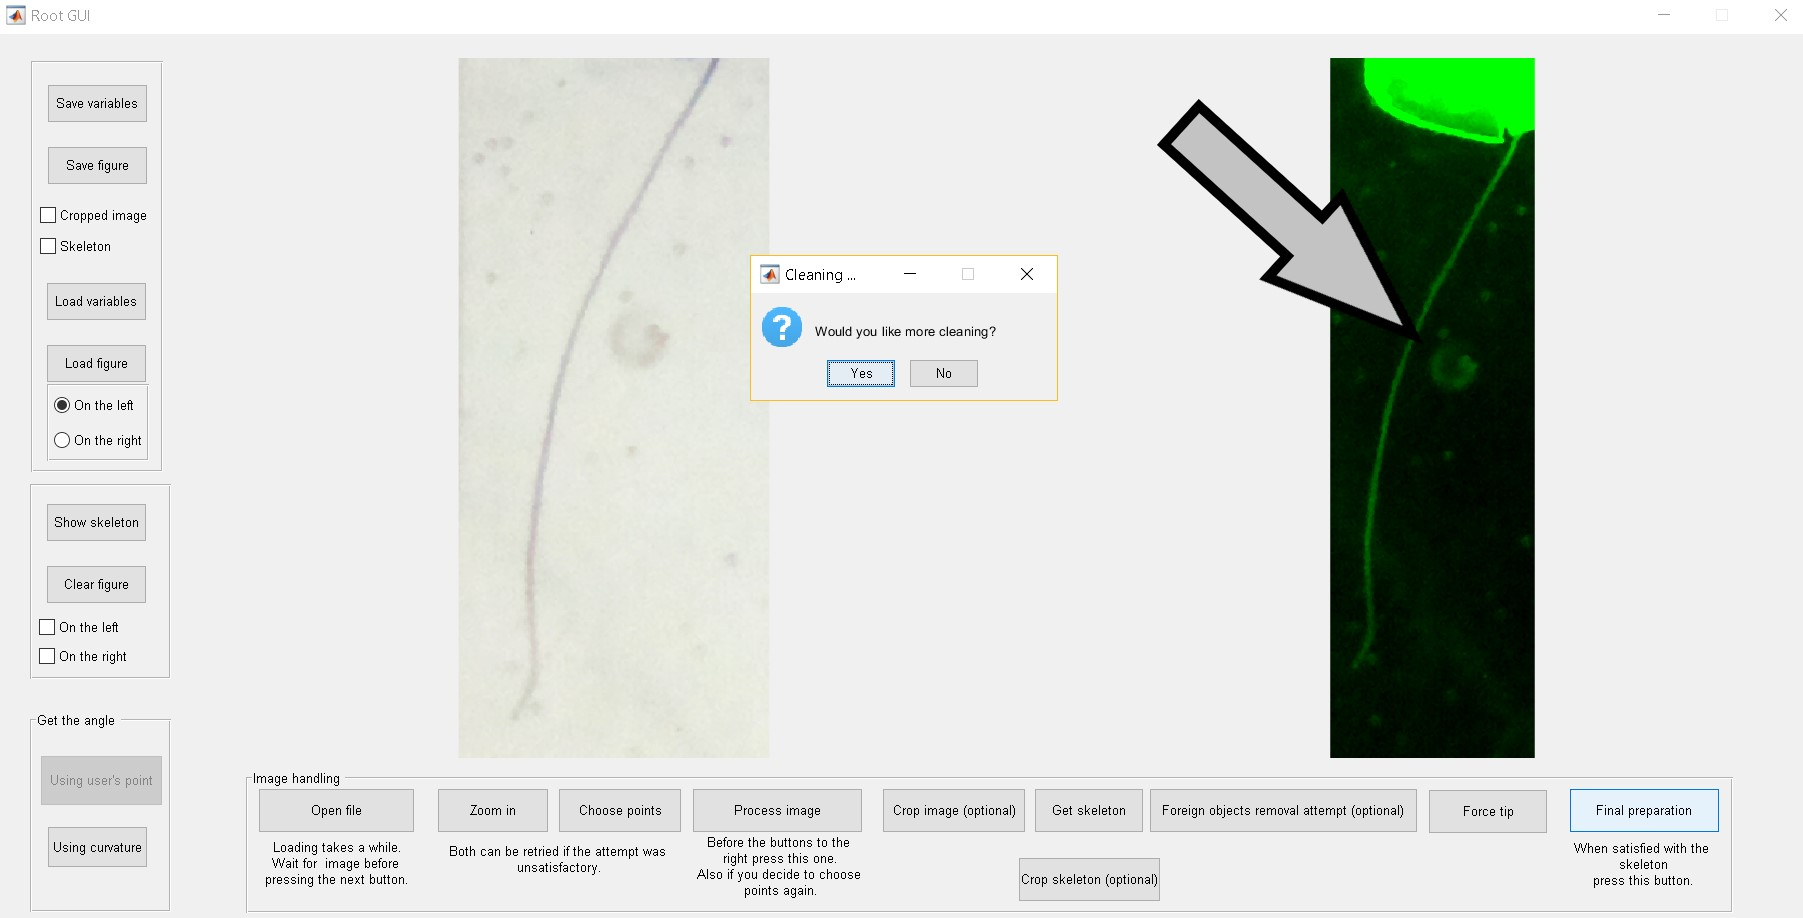
\includegraphics[width=\textwidth]{../Figures/manual/optionalA4.jpg}
	\caption{Prompt for futher cleaning when root is gone}
	\label{fig:img33}
\end{figure}

\begin{figure}[H]
	\centering
	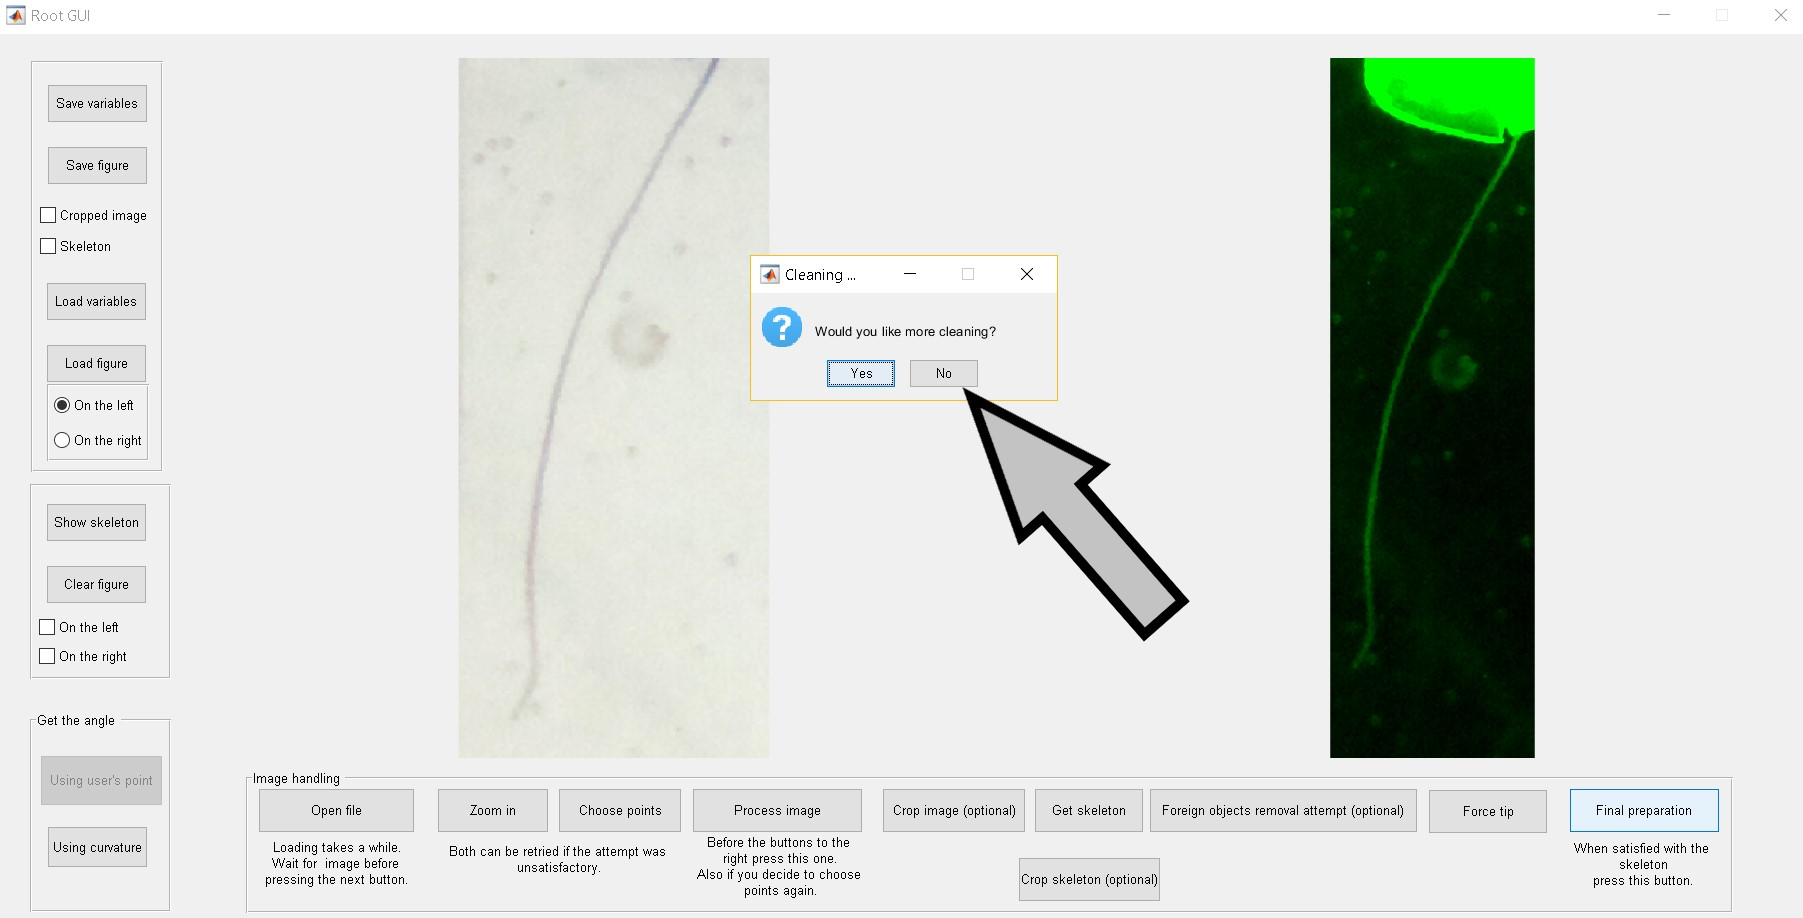
\includegraphics[width=\textwidth]{../Figures/manual/optionalA5.jpg}
	\caption{Clicking 'No' upon prompt for further cleaning}
	\label{fig:img34}
\end{figure}

\begin{figure}[H]
	\centering
	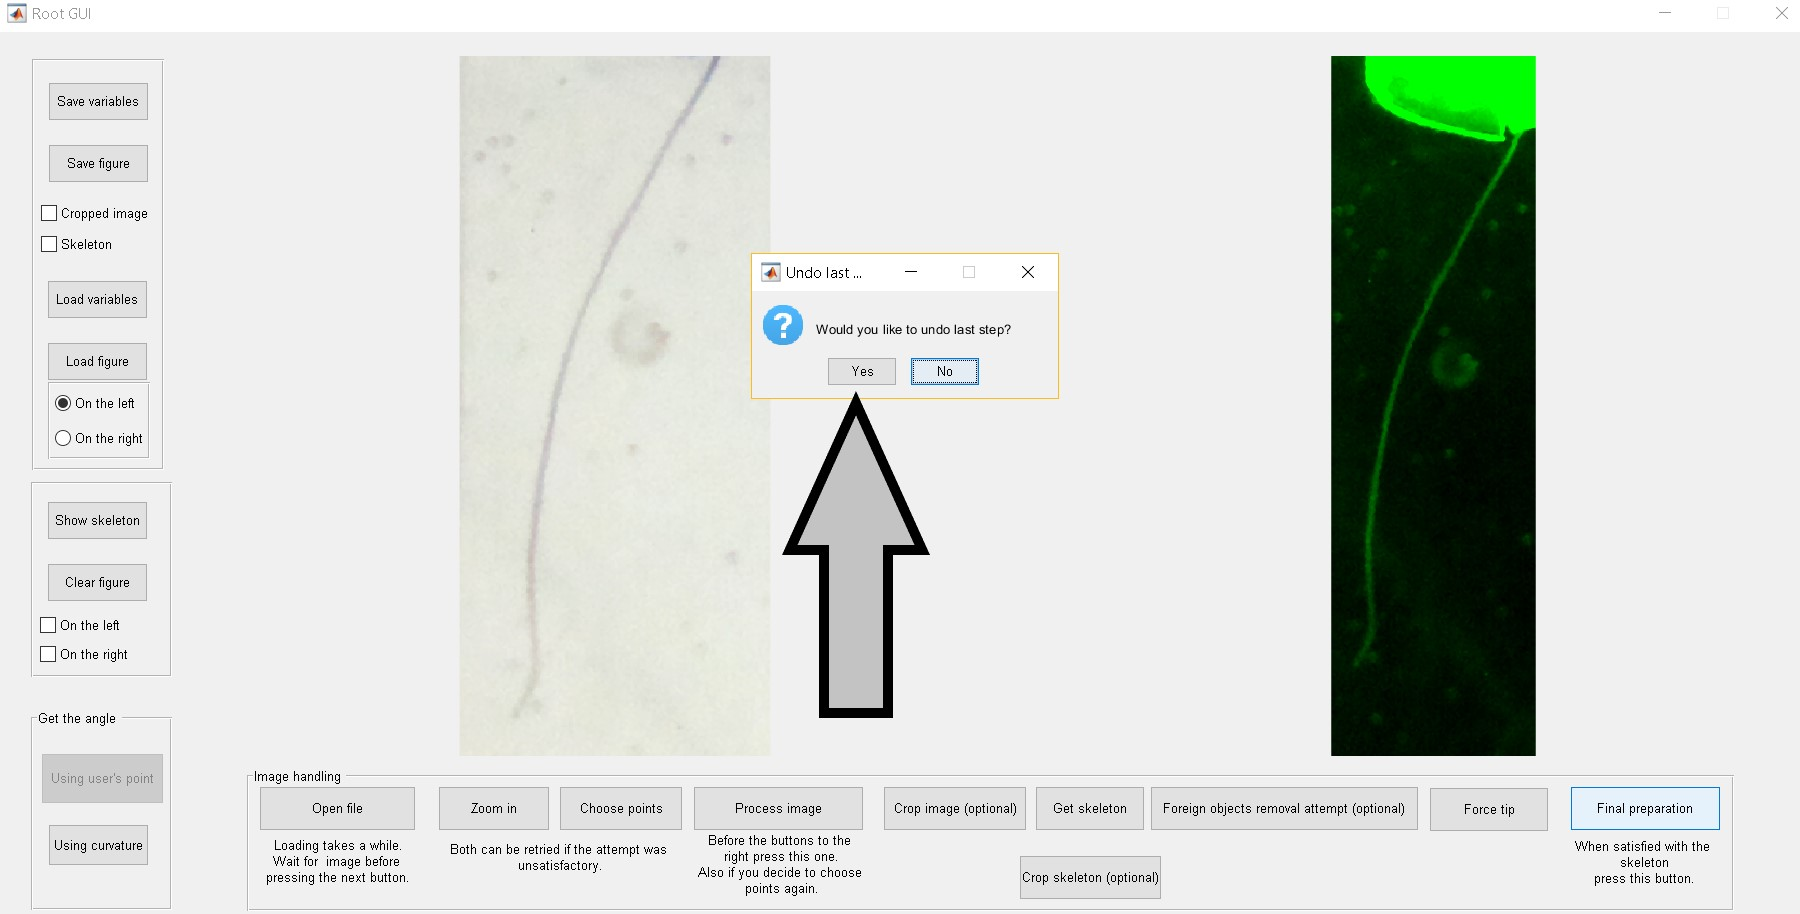
\includegraphics[width=\textwidth]{../Figures/manual/optionalA6.jpg}
	\caption{Clicking 'Yes' when asked to undo last step}
	\label{fig:img35}
\end{figure}

As you can see in figure \ref{fig:img36}, the skeleton "came back".

\begin{figure}[H]
	\centering
	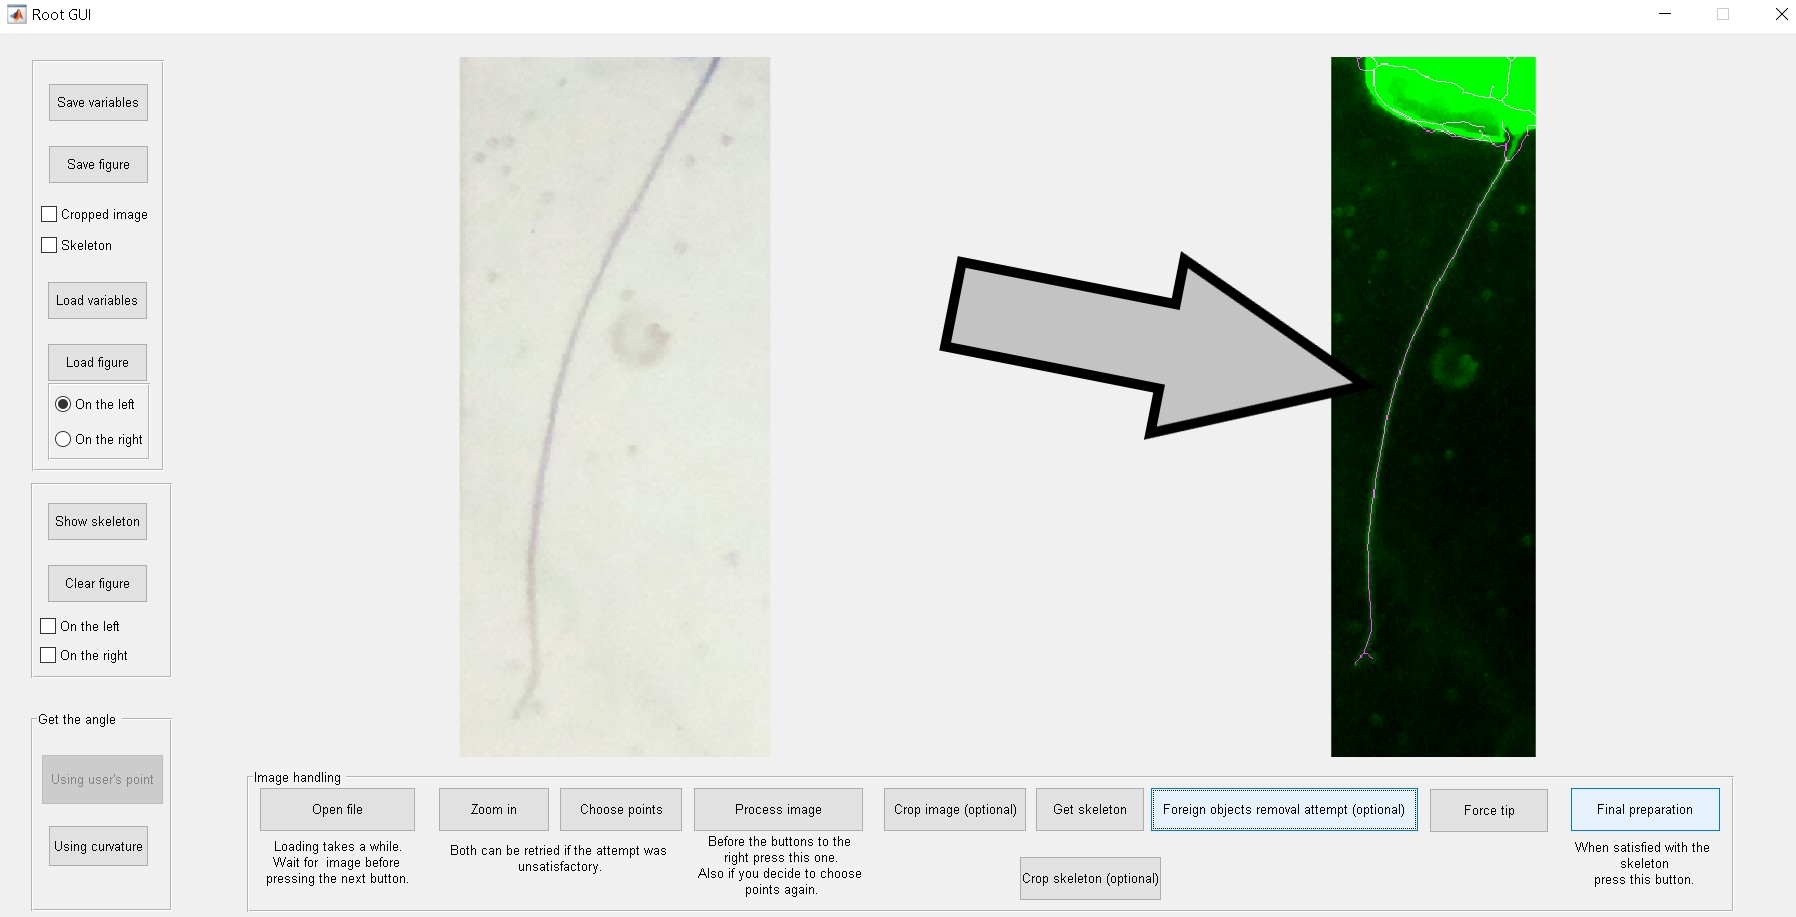
\includegraphics[width=\textwidth]{../Figures/manual/optionalA7.jpg}
	\caption{Upon undoing the last step the skeleton came back}
	\label{fig:img36}
\end{figure}


%----------------------------------------------------------------------------------------
\subsection{Force tip}

There a still various problems that can crop up but they can be solved.
For example, what if the skeleton you got doesnt't get all the way to the tip of the root? 
Well, that's a task for \textit{Force tip}, that enforces the tip of the root to be contained in the skeleton. 
So first you click the button \textit{Force tip} (see figure \ref{fig:img37}, then a message pops up asking you to drag a iine from the end of the skeleton to the tip (see figure \ref{fig:img38}).
But we can actually do it in more than one step. For example, in the example given here it seems like a straight line from the skeleton to the tip won't follow the root. 
So let's first do the short line on figure \ref{fig:img39}, then to see how it looks, we can click on \textit{Show skeleton} (see figures \ref{fig:img40} -- \ref{fig:img41}),
and we'll see the skeleton alone on the left and overlaid on the root on the right. 
And then, we'll draw the final line (see figure \ref{fig:img42}).
We'll click on \textit{Show skeleton} again to see if we are pleased (see figure \ref{fig:img43}), then on \textit{Final preparation} and we'll see that we go a reasonable angle (see figures \ref{fig:img44} -- \ref{fig:img45}).


\begin{figure}[H]
	\centering
	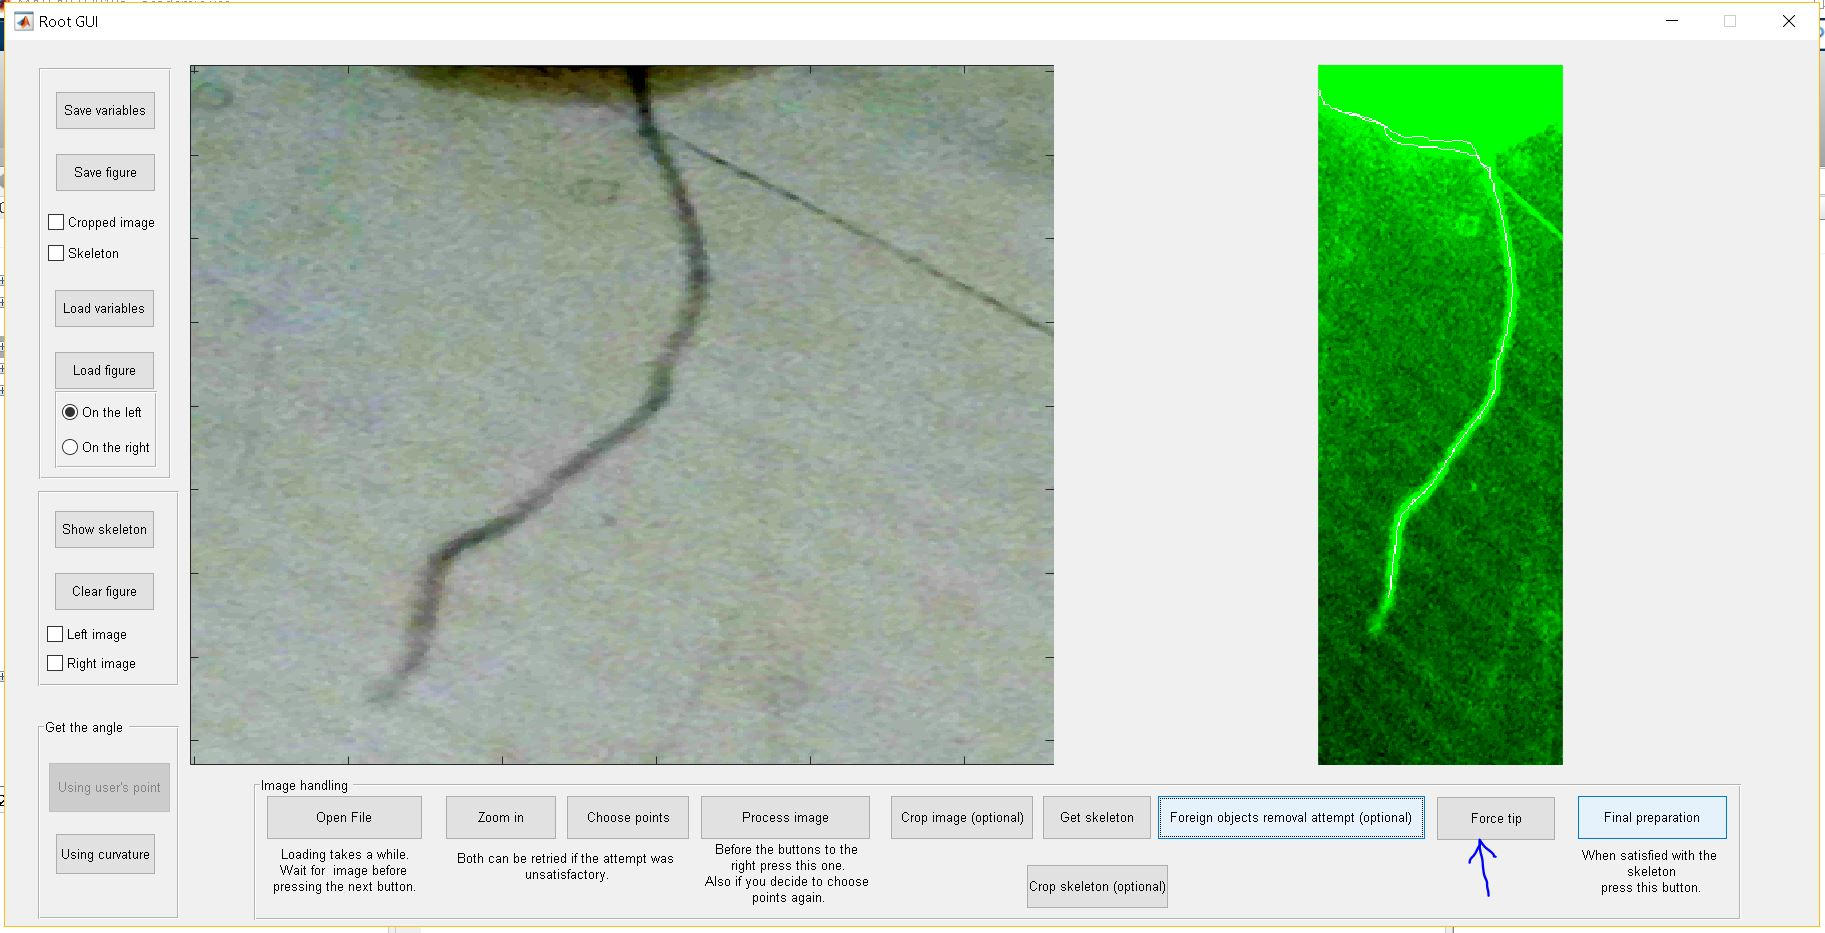
\includegraphics[width=\textwidth]{../Figures/manual/optionalB1.jpg}
	\caption{Optional step in the \textit{RootSkel} pipeline: Force tip}
	\label{fig:img37}
\end{figure}

\begin{figure}[H]
	\centering
	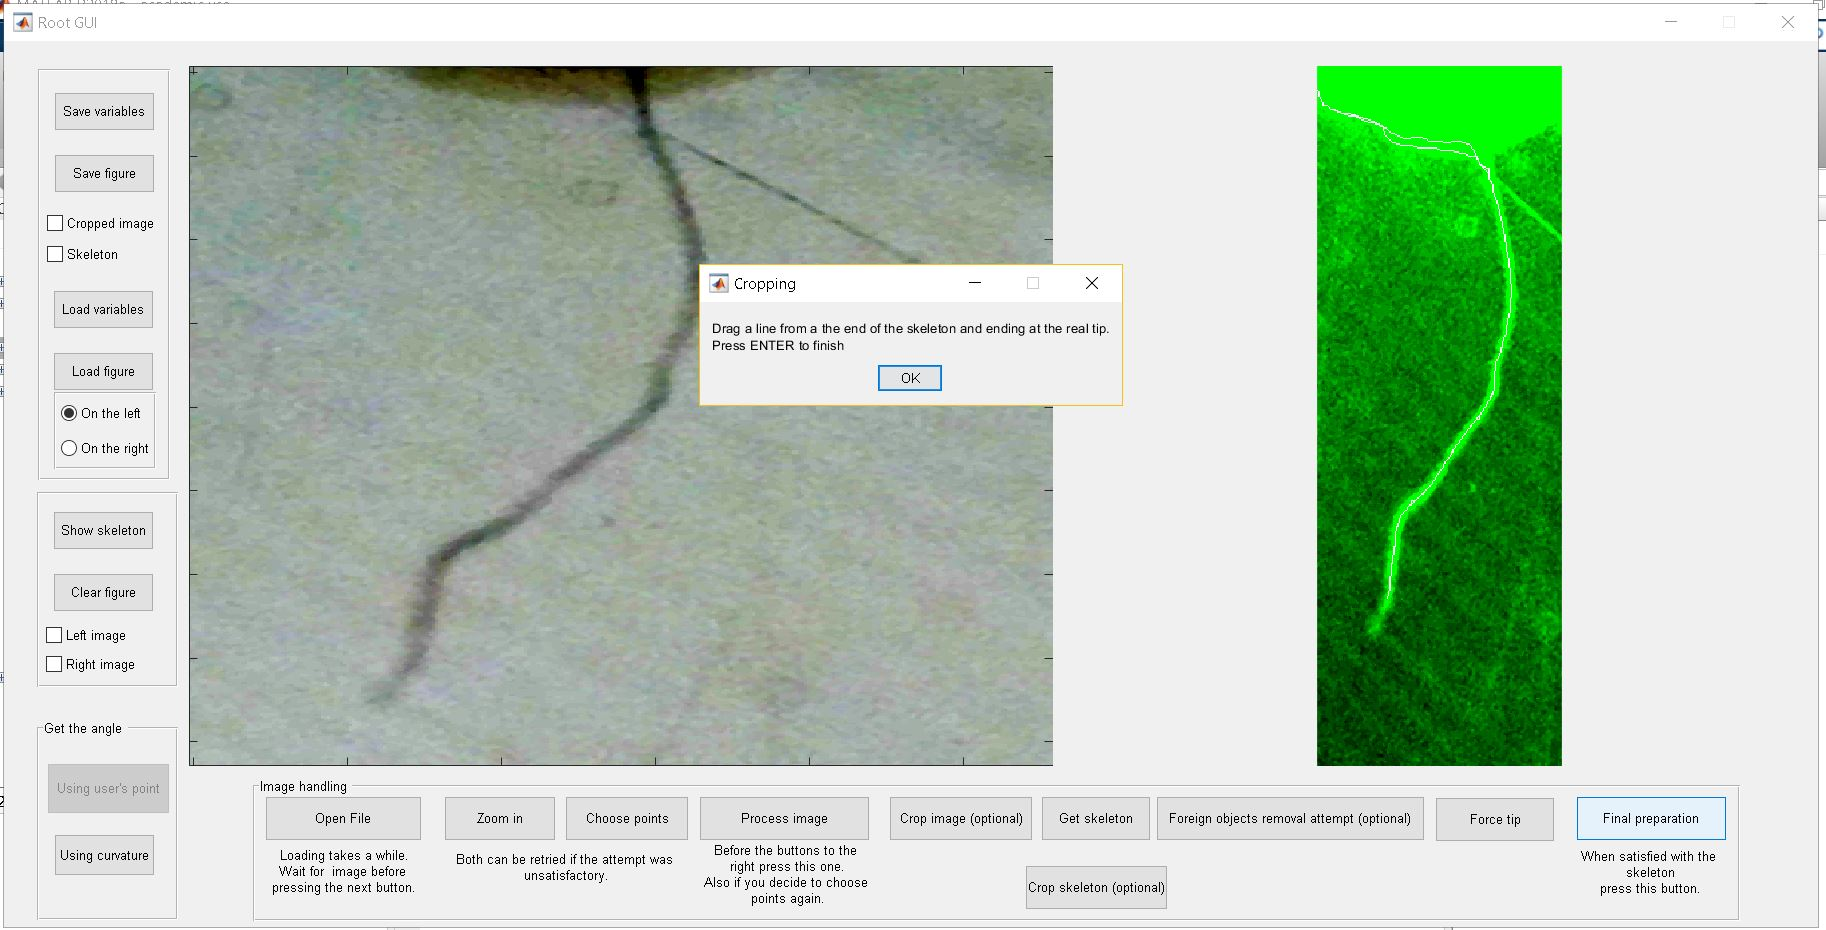
\includegraphics[width=\textwidth]{../Figures/manual/optionalB2.jpg}
	\caption{Instructions upon clicking on \textit{Force tip}}
	\label{fig:img38}
\end{figure}

\begin{figure}[H]
	\centering
	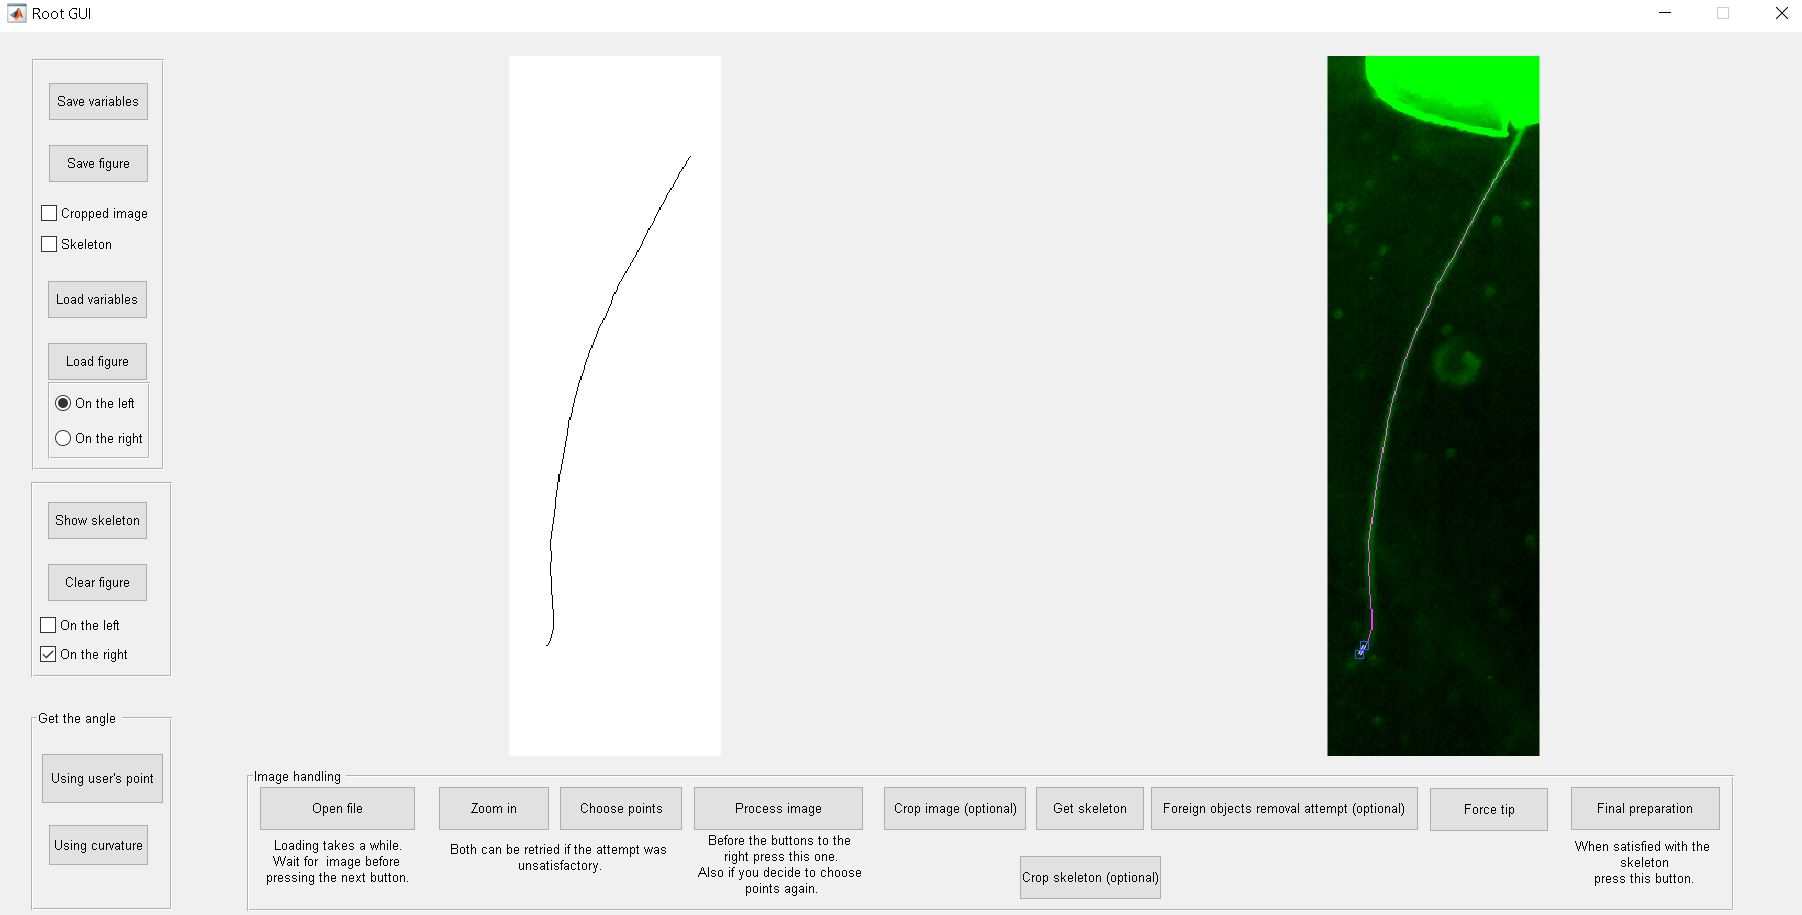
\includegraphics[width=\textwidth]{../Figures/manual/optionalB3.jpg}
%	\caption{Applying \textit{force tip}: Elongating the tip of the root skeleton}
%	\caption{Applying \textit{force tip}: Trying to elongate the tip of the root with a line}
	\label{fig:img39}
\end{figure}

\begin{figure}[H]
	\centering
	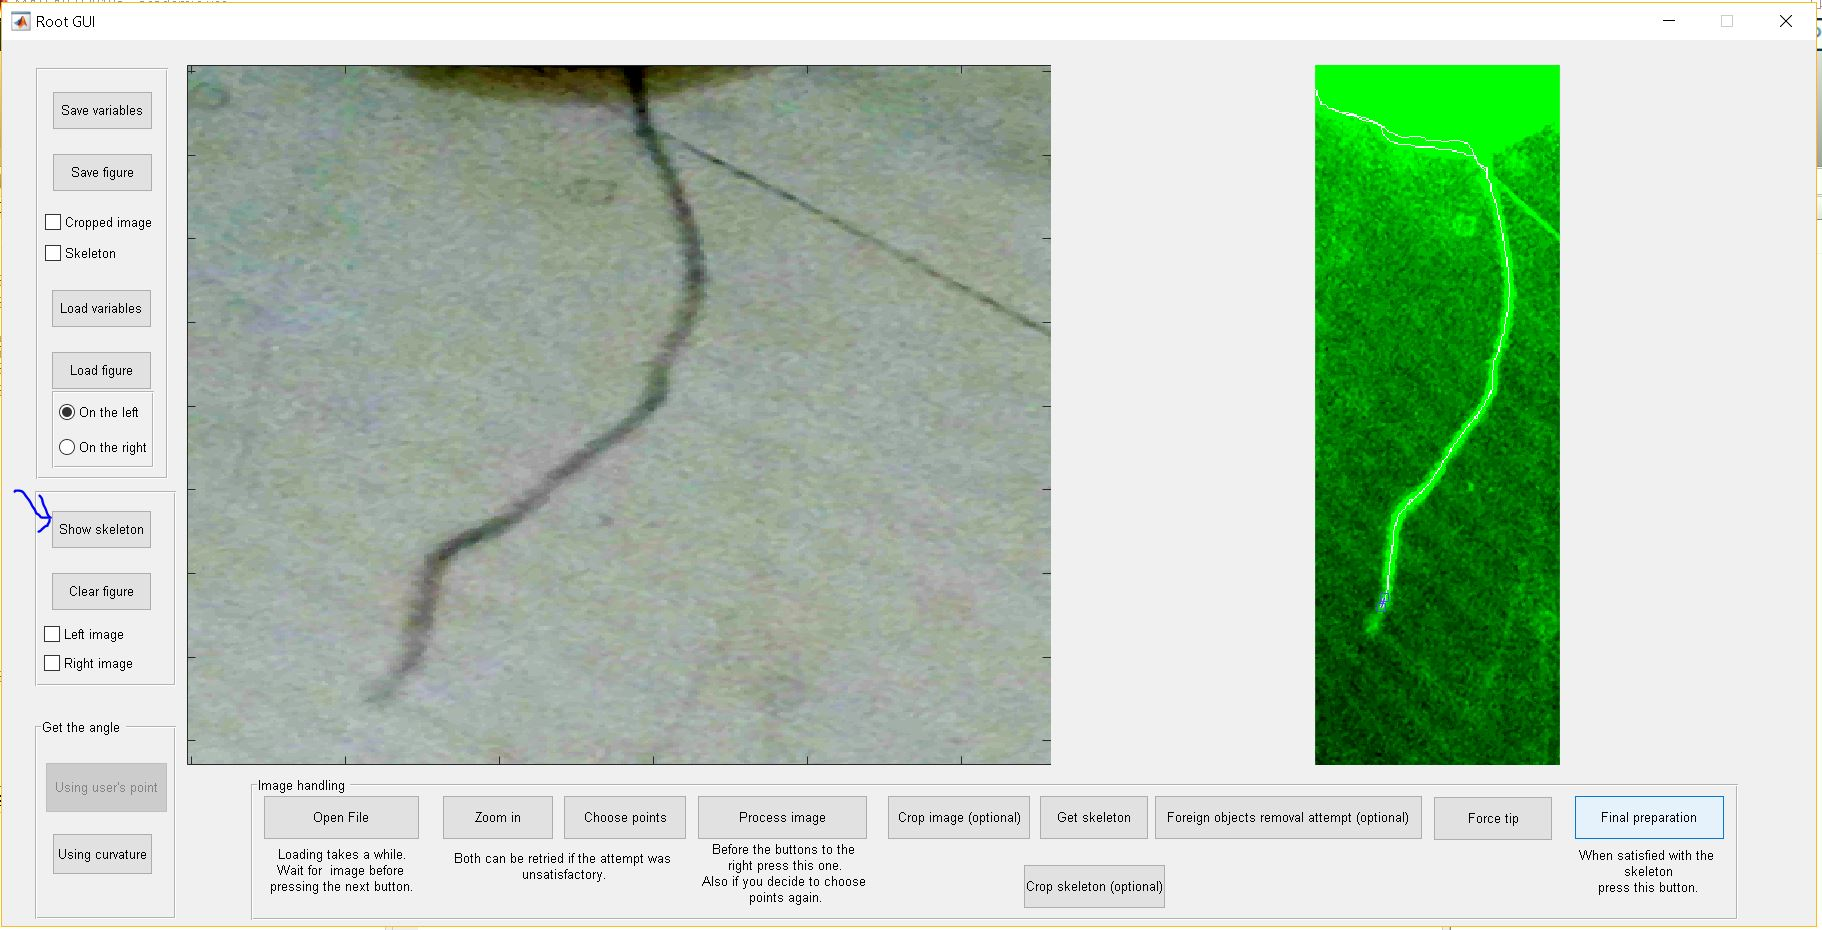
\includegraphics[width=\textwidth]{../Figures/manual/optionalB4.jpg}
	\caption{Clicking on \textit{Show skeleton} to show the new skeleton}
	\label{fig:img40}
\end{figure}

\begin{figure}[H]
	\centering
	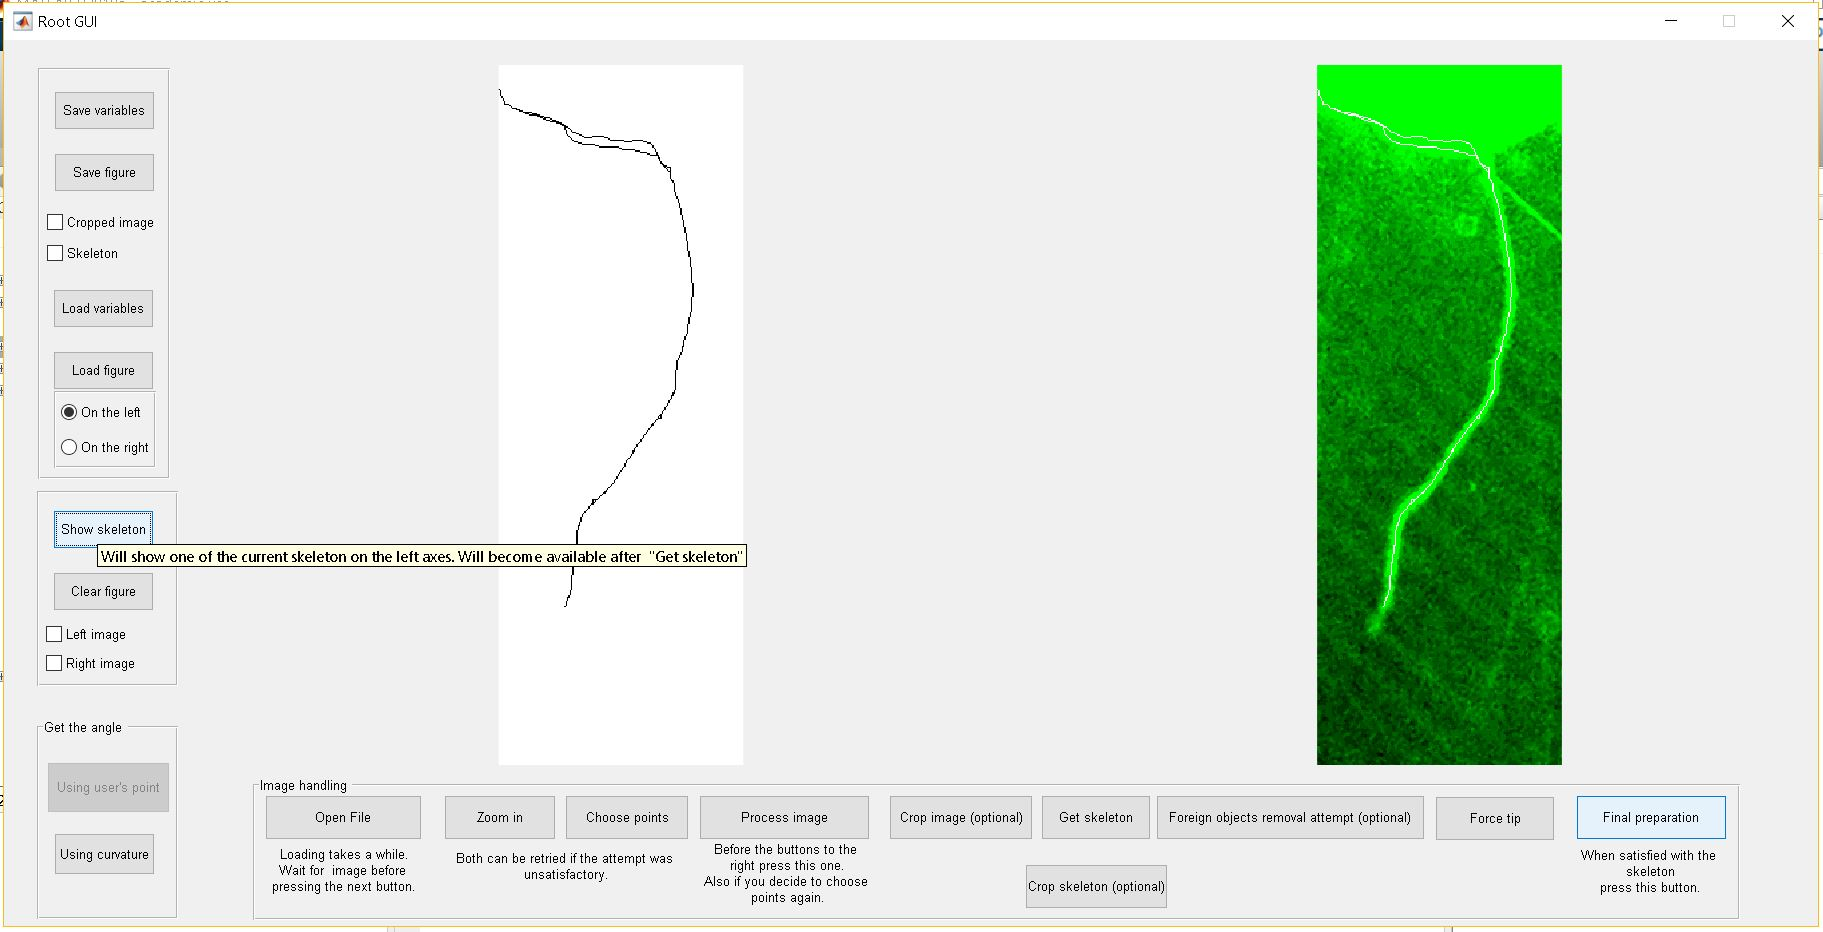
\includegraphics[width=\textwidth]{../Figures/manual/optionalB5.jpg}
	\caption{Message upon hovering over the \textit{Show skeleton} button}
	\label{fig:img41}
\end{figure}

\begin{figure}[H]
	\centering
	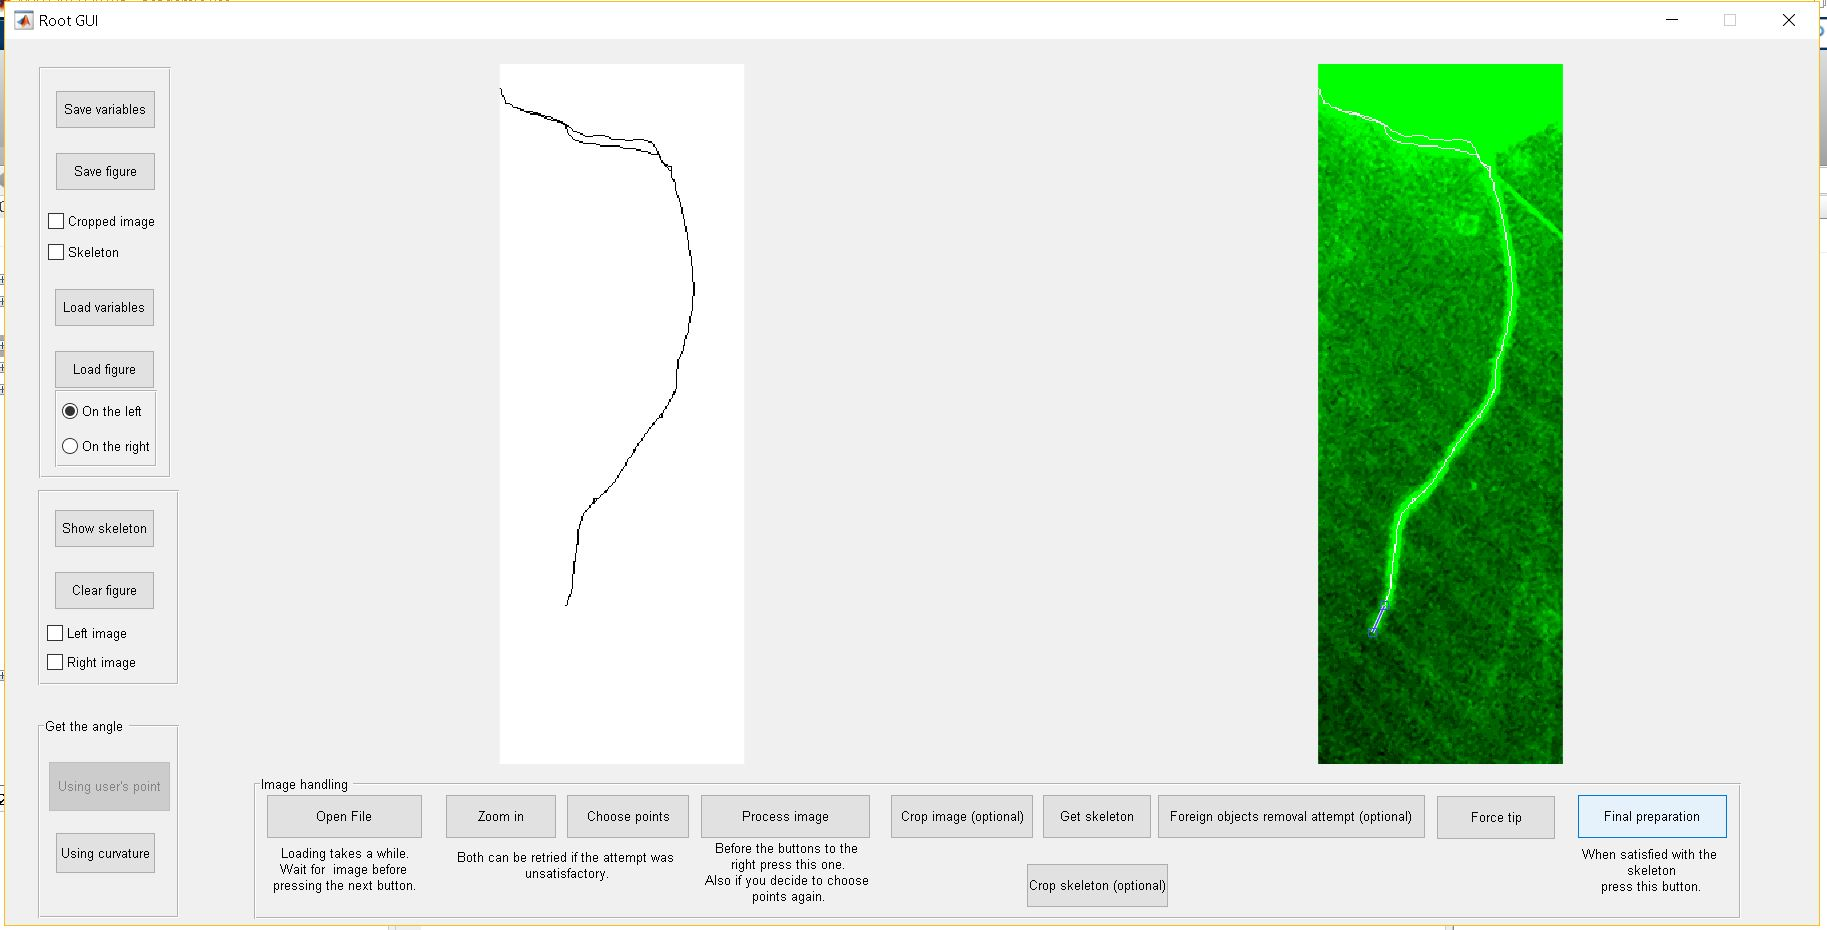
\includegraphics[width=\textwidth]{../Figures/manual/optionalB6.jpg}
	\caption{The current skeleton}
	\label{fig:img42}
\end{figure}

\begin{figure}[H]
	\centering
	\includegraphics[width=\textwidth]{../Figures/manual/optionalB7.jpg}
%    \caption{Applying \textit{force tip}: Trying to elongate the tip of the root with a line}
	\caption{Upon clicking \textit{Show skeleton}: The elongated tip skeleton}
	\label{fig:img43}
\end{figure}

\begin{figure}[H]
	\centering
	\includegraphics[width=\textwidth]{../Figures/manual/optionalB8.jpg}
	\caption{Clicking 'No' when asked to optionally choose a point of highest local (mean) curvature}
	\label{fig:img44}
\end{figure}

\begin{figure}[H]
	\centering
	\includegraphics[width=\textwidth]{../Figures/manual/optionalB9.jpg}
	\caption{The calculated angle in a pop up window}
	\label{fig:img45}
\end{figure}


%----------------------------------------------------------------------------------------
\subsection{Crop image}

Let's say we have a problem like the one in figure \ref{fig:img46}.

\begin{figure}[H]
	\centering
	\includegraphics[width=\textwidth]{../Figures/manual/optionalC1.jpg}
	\caption{Unwanted branches in the root skeleton}
	\label{fig:img46}
\end{figure}

\begin{figure}[H]
	\centering
	\includegraphics[width=\textwidth]{../Figures/manual/optionalC2.jpg}
	\caption{Optional step in the \textit{RootSkel} pipeline: Crop image}
	\label{fig:img47}
\end{figure}

\begin{figure}[H]
	\centering
	\includegraphics[width=\textwidth]{../Figures/manual/optionalC3.jpg}
	\caption{Prompt upon clicking on \textit{Crop image}}
	\label{fig:img48}
\end{figure}

\begin{figure}[H]
	\centering
	\includegraphics[width=\textwidth]{../Figures/manual/optionalC4.jpg}
	\caption{Highlighted problematic regions that need cropping}
	\label{fig:img49}
\end{figure}

\begin{figure}[H]
	\centering
	\includegraphics[width=\textwidth]{../Figures/manual/optionalC5.jpg}
	\caption{Prompt to redo the cropping}
	\label{fig:img50}
\end{figure}

\begin{figure}[H]
	\centering
	\includegraphics[width=\textwidth]{../Figures/manual/optionalC6.jpg}
	\caption{New problems in the skeleton that requires another round of cropping}
	\label{fig:img51}
\end{figure}

\begin{figure}[H]
	\centering
	\includegraphics[width=\textwidth]{../Figures/manual/optionalC7.jpg}
	\caption{Clicking on the optional step \textit{Crop image} for more cropping}
	\label{fig:img52}
\end{figure}

\begin{figure}[H]
	\centering
	\includegraphics[width=\textwidth]{../Figures/manual/optionalC8.jpg}
	\caption{Prompt to redo the cropping after the second attempt}
	\label{fig:img53}
\end{figure}

\begin{figure}[H]
	\centering
	\includegraphics[width=\textwidth]{../Figures/manual/optionalC9.jpg}
	\caption{No problems close to the root tip, only further up}
	\label{fig:img54}
\end{figure}

We still have these weird branches. But since they are not any close to the root and it seems like the skeleton near the tip is following the root, I think it's time we switch tactics.

%----------------------------------------------------------------------------------------
\subsection{Crop skeleton}

So now, the main problem we have is only the existence of these branches, and less the effect on the shape of the skeleton near the tip. For such problems, the \textit{Get skeleton} step was developed. 

Let's trim some branches! Click on the \textit{Get skeleton} button and you will see our trusty instruction pop up (see figures \ref{fig:img55} -- \ref{fig:img56}).
Now, there is no rush, we can trim the branches one by one. So first, we'll trim the left branch (see figure \ref{fig:img57}), and then we will click 'No' followes by another click on \textit{Get skeleton}, after which we trim the second branch which leaves us with a nice and clean skeleton (see figures \ref{fig:img58} -- \ref{fig:img59}).
To see the result, we will click \textit{Final preparation} followed by \textit{Using curvature} and we see that we are getting a reasonable result (see figures \ref{fig:img60} -- \ref{fig:img61}). Success!


\begin{figure}[H]
	\centering
	\includegraphics[width=\textwidth]{../Figures/manual/optionalD1.jpg}
	\caption{Optional step in the \textit{RootSkel} pipeline: Crop skeleton}
	\label{fig:img55}
\end{figure}

\begin{figure}[H]
	\centering
	\includegraphics[width=\textwidth]{../Figures/manual/optionalD2.jpg}
	\caption{Instructions upon clicking on \textit{Crop skeleton}}
	\label{fig:img56}
\end{figure}

\begin{figure}[H]
	\centering
	\includegraphics[width=\textwidth]{../Figures/manual/optionalD3.jpg}
	\caption{Prompt to redo the cropping}
	\label{fig:img57}
\end{figure}

\begin{figure}[H]
	\centering
	\includegraphics[width=\textwidth]{../Figures/manual/optionalD4.jpg}
	\caption{A perfectly cropped root}
	\label{fig:img58}
\end{figure}

\begin{figure}[H]
	\centering
	\includegraphics[width=\textwidth]{../Figures/manual/optionalD5.jpg}
	\caption{Another nice and clean skeleton}
	\label{fig:img59}
\end{figure}

\begin{figure}[H]
	\centering
	\includegraphics[width=\textwidth]{../Figures/manual/optionalD6.jpg}
	\caption{Clicking \textit{Final preparation} and \textit{Using curvature} to compute the angle on the new skeleton}
	\label{fig:img60}
\end{figure}

\begin{figure}[H]
	\centering
	\includegraphics[width=\textwidth]{../Figures/manual/optionalD7.jpg}
	\caption{Message box displaying the computed angle}
	\label{fig:img61}
\end{figure}


%----------------------------------------------------------------------------------------
\subsection{Giving the problem a turning point}

For our last optional step, remember that pop up window when we click \textit{Final preparation}? The one I said we will come back to?
Well it's about time we do! So we go back to \textit{Final preparation}, only this time we will click 'Yes' when prompted (see figures \ref{fig:img62} -- \ref{fig:img63}).
Now the instructions will pop up asking us to choose the point of maximum local curvature near the tip, so we will do just that and press ENTER (see figures \ref{fig:img64} -- \ref{fig:img65}). Now a new button is enabled (see figure \ref{fig:img66}).

So we will click \textit{Using user's point} and then a message will pop up (see figure \ref{fig:img67}) with the angle and a new file will be created (see figure \ref{fig:img68}).
And that's it! We are done here! Hope you've enjoyed this friendly manual, and see you next time. 

\begin{figure}[H]
	\centering
	\includegraphics[width=\textwidth]{../Figures/manual/optionalE1.jpg}
	\caption{Last step in the \textit{RootSkel} pipeline: Final preparation}
	\label{fig:img62}
\end{figure}

\begin{figure}[H]
	\centering
	\includegraphics[width=\textwidth]{../Figures/manual/optionalE2.jpg}
	\caption{Prompt to choose the point of highest local curvature (optional)}
	\label{fig:img63}
\end{figure}

\begin{figure}[H]
	\centering
	\includegraphics[width=\textwidth]{../Figures/manual/optionalE3.jpg}
	\caption{Instructions to choose the point of highest local curvature}
	\label{fig:img64}
\end{figure}

\begin{figure}[H]
	\centering
	\includegraphics[width=\textwidth]{../Figures/manual/optionalE4.jpg}
	\caption{Choosing the point of highest local curvature}
	\label{fig:img65}
\end{figure}

\begin{figure}[H]
	\centering
	\includegraphics[width=\textwidth]{../Figures/manual/optionalE5.jpg}
	\caption{Clicking on \textit{Using users input} upon clicking on the point of highest local curvature}
	\label{fig:img66}
\end{figure}

\begin{figure}[H]
	\centering
	\includegraphics[width=\textwidth]{../Figures/manual/optionalE6.jpg}
	\caption{Message box displaying the computed angle}
	\label{fig:img67}
\end{figure}

\begin{figure}[H]
	\centering
	\includegraphics[width=0.6\textwidth]{../Figures/manual/optionalE7.jpg}
	\caption{The created .csv files with the computed angles showing up on the RHS of the MATLAB GUI}
	\label{fig:img68}
\end{figure}


%----------------------------------------------------------------------------------------
%----------------------------------------------------------------------------------------
%----------------------------------------------------------------------------------------
\chapter{On the data set}

The data set used can be found on \url{https://imperialcollegelondon.app.box.com/folder/50485327378}.

%----------------------------------------------------------------------------------------
%----------------------------------------------------------------------------------------
\section{Suggestions for future data acquisition}

We will give some suggestions on how to improve the quality of the images in the future.


%----------------------------------------------------------------------------------------
\subsection{Stable conditions in the experiment}

In general, one should ensure to keep the conditions over one experiment stable as far as possible. It should be noted that this is far harder to achieve in a dynamic system as the one to capture electrotropism compared to a gravitropism setup; the latter usually being done in a stabilising agar gel. 
This includes a constant number of tubes and roots, constant water level or surface and no external movement to the roots or the tubes to keep the noise distribution as constant as possible. Roots that are affected by change in reflections or illumination (e.g. by people walking into the room) have been proven to be very hard to handle and are often lost in the preprocessing step. 
Keeping the medium clean of dirt and bubbles as far as possible will also improve the preprocessing step. 


\subsection{No objects interfering with the object of interest}

The experimentalist should make sure that there are no objects interfering with the object of interest, be it other roots or any other similar looking objects that are hard to discern even by eye, throughout the experiment.

%llumination different — challenge to get background right
%local thresholds maybe?


%----------------------------------------------------------------------------------------
\subsection{Increase of the contrast}

It is advisable to work towards achieving a higher contrast in the images, so roots can be clearly distinguished from the background, also by eye.


%%----------------------------------------------------------------------------------------
%\subsection{More focus on images}


%----------------------------------------------------------------------------------------
\subsection{Higher resolution}


As the highly pixeled nature of the images did cause problems also in the angle computation, it is recommendable to try to increase the resolution of the images (e.g. to 10 Mexapixels, in the current images we use 5-8 Megapixels, that is dimensions between 3280\(\times\)2464 and 2592\(\times\)1944). We could also try to zoom into the roots or even one single root so our actual object(s) of interest take a bigger fraction in the images instead of spending resolution on things that are of no interest. 

It might also be the lossy compression (i.e. we cannot recover the original image) step into .JPG file format after taking the photos which creates coarser images and details to be removed.
%that might cause or contribute to the low resolution of the images. 
One could attempt to use other formats to save the images, including lossless formats such as PNG file format.

As a last suggestion, different cameras could be compared to see if it does have an effect on the quality of the images. 

%Better camera, less waste of resolution
%improve spatial resolution, other format? no compression?


%----------------------------------------------------------------------------------------
%----------------------------------------------------------------------------------------
%----------------------------------------------------------------------------------------
\chapter{Literature review}\label{litreview}

%\include{Appendices/AppendixB}
%\include{Appendices/AppendixC}

\end{document}  
